%\documentclass[bibtotoc,liststotoc,BCOR5mm,DIV12]{scrbook}
\documentclass[bibtotoc,liststotoc,BCOR5mm,DIV12,oneside]{scrbook}
% use this declaration to set specific page margins
%\usepackage[a4paper , lmargin = {4cm} , rmargin = {2cm} , tmargin = {2cm} , bmargin = {4cm} ]{geometry}
\usepackage[a4paper]{geometry}
% \usepackage{titlesec}
% \setcounter{secnumdepth}{4}
% \usepackage{subcaption}
\usepackage{float}
\usepackage[ngerman, english]{babel}
\usepackage{bibgerm}       	   % german references
\usepackage[utf8]{inputenc}  % german characters
\usepackage{graphicx} 				% it's recommended to use PDF images but you can use JPG or PNG as well
\usepackage{url}           		% format URLs
\def\UrlBreaks{\do\/\do-}
\usepackage{hyperref} 				% create hyperlinks
\usepackage{listings, color}	% for source code
\usepackage{subfig}						% two figures next to each other (example: figure 3a), figure 3b)
\usepackage{scrpage2}					% header and footer line
\usepackage{array}
\usepackage{amsmath}
\usepackage[table]{xcolor} % color for the cell
\usepackage[section]{placeins}


%\usepackage{multirow}
\newcolumntype{P}[1]{>{\centering\arraybackslash}p{#1}}
% header and footer line - no header & footer line on pages where a new chapter starts
\pagestyle{scrheadings}
\chead{\rightmark}
\ihead{}
\ohead{}
%\ihead{Muhammad Ahsan Shahid}
\ofoot[]{}
\ifoot{}
\cfoot{\thepage}
%\ifoot{Master Thesis, TU Berlin, Faculty IV, 2019}

%\ifoot{Diploma Thesis, TU Berlin, Fachgebiet AV, 2009}

% set path where images are stored
\graphicspath{{./img/}}
%
% der Befehl \hypenation versteht keine Sonderzeichen, also weder ä
% noch "a noch \"a. Wörter die derartige Zeichen enthalten müssen
% direkt im Text getrennt werden, z.B. Wör\-ter
%
\hyphenation{te-le-com-muni-cation 
te-le-com-muni-cation-specific 
Te-le-kom-mu-ni-ka-tions-API} 					% use this file to set explicit hyphenations (doesn't seem to work correctly)
\setcounter{tocdepth}{3}
\setcounter{secnumdepth}{5}

% For quotations
\usepackage{epigraph}

% For json
% \usepackage{bera}% optional: just to have a nice mono-spaced font
\usepackage{listings}
\usepackage{xcolor}

\colorlet{punct}{red!60!black}
\definecolor{background}{HTML}{EEEEEE}
\definecolor{delim}{RGB}{20,105,176}
\colorlet{numb}{magenta!60!black}

\lstdefinelanguage{json}{
    basicstyle=\small,
    % \normalfont\ttfamily,
    numbers=left,
    numberstyle=\scriptsize,
    stepnumber=1,
    numbersep=8pt,
    showstringspaces=false,
    breaklines=true,
    frame=lines,
    captionpos=b,
    backgroundcolor=\color{background},
    literate=
     *{0}{{{\color{numb}0}}}{1}
      {1}{{{\color{numb}1}}}{1}
      {2}{{{\color{numb}2}}}{1}
      {3}{{{\color{numb}3}}}{1}
      {4}{{{\color{numb}4}}}{1}
      {5}{{{\color{numb}5}}}{1}
      {6}{{{\color{numb}6}}}{1}
      {7}{{{\color{numb}7}}}{1}
      {8}{{{\color{numb}8}}}{1}
      {9}{{{\color{numb}9}}}{1}
      {:}{{{\color{punct}{:}}}}{1}
      {,}{{{\color{punct}{,}}}}{1}
      {\{}{{{\color{delim}{\{}}}}{1}
      {\}}{{{\color{delim}{\}}}}}{1}
      {[}{{{\color{delim}{[}}}}{1}
      {]}{{{\color{delim}{]}}}}{1},
}

% \usepackage[toc,page]{appendix} %for appendix
\usepackage{pdfpages}

\begin{document}
% ---------------------------------------------------------------
\frontmatter
    \thispagestyle{empty}
\begin{center}

\vspace*{1cm}
{\LARGE \textbf{Technische Universität Berlin}}

\vspace{0.5cm}

{\large Institute of Software Engineering and Theoretical Computer Science\\[1mm]}
{\large Quality and Usability Lab\\[5mm]}

Fakultät IV\\
Einsteinufer 17\\
10587 Berlin\\
www.eecs.tu-berlin.de\\

\vspace*{0.8cm}


\includegraphics[width=4cm]{tu_logo.jpg}

\vspace*{0.8cm}

{\LARGE Master Thesis}\\

\vspace{0.8cm}
{\LARGE \textbf{Implementation of a Framework for the Rapid Development of Conversational Interfaces}}\\
\vspace*{1.0cm}
{\LARGE Muhammad Ahsan Shahid}
\\
\vspace*{0.5cm}
Matriculation Number: 0389868\\
09.07.2020\\  % 	date of submission
\vspace*{0.8cm}

Examiner: Prof. Dr.-Ing. Sebastian Möller\\
\vspace*{0.4cm}
Second Examiner: Prof. Dr. Axel Küpper\\
\vspace*{0.4cm}
Supervisors:\\
Dr.-Ing. Stefan Hillmann\\
M.SC. Jan Nehring
\vspace*{0.4cm}




\end{center}

   	\thispagestyle{empty}
    \cleardoublepage
    
   \thispagestyle{empty}
\vspace*{3cm}

\begin{center}
\textbf{Acknowledgment}
\end{center}

\vspace*{0.5cm}
\\~\\
Primarily, I would like to thank my supervisor Prof. Dr. Ing. Sebastian Möller for giving me the opportunity to accomplish the research under his excellent supervision. I am also grateful to Prof. Dr. Axel Küpper for the help and support as a second supervisor of my thesis.
\\~\\
I am deeply grateful to Stefan Hillman from Technische Universität Berlin and Jan Nehring from DFKI-German Research Centre for Artificial Intelligence, for arranging regular meetings to check with the progress and providing every possible help. I am really thankful to both of them for having constructive discussions and thorough guidance throughout a hard time, that pushed me to achieve this accomplishment.
\\~\\
I would like to thank my friends and all the people that have spared the time to read this thesis and provided me valuable feedback.
   \thispagestyle{empty}
   \cleardoublepage
    
    \newpage

\thispagestyle{empty}

\begin{large}

\vspace*{6cm}

\noindent
I hereby declare that the thesis submitted is my own, unaided work, completed
without any un-permitted external help. Only the sources and resources listed were
used.
\\
\\

\noindent
Place, Date
\\

\noindent
Berlin, 12.07.2020

\vspace{3cm}

\hspace*{9cm}%
\dotfill\\
\hspace*{8.5cm}%
\textit{(Signature [Muhammad Ahsan Shahid])}

\end{large}
 
    \thispagestyle{empty}
    \cleardoublepage
    
    
    \thispagestyle{empty}
\vspace*{1.0cm}

\begin{center}
    \textbf{Abstract}
\end{center}

\vspace*{0.5cm}

\noindent
The trend of developing chatbots at a corporate level has been raised for the last few years. The existing state of the art dialogue frameworks like IBM's Watson Assistant \cite{ibmwatson}, RASA \cite{rasa}, and PLATO \cite{plato} are providing great support in this regard. But still there exist various hindrances that need to be addressed in order to make this emerging technology noticeable. It is necessary to keep the frameworks as simple as possible without compromising on its abilities so that a non-technical person could also be able to develop a chatbot according to his/her needs.
\\~\\
This thesis illustrates the design, implementation, and evaluation of the chatbot framework developed using novel Modular Architecture. The chatbot designed using this framework is named as "Frankenbot". The chatbot uses the RASA's Natural Language Understanding(NLU) Model for the semantical interpretation of the users' utterances in order to fetch the required fields for the chatbot. 
\\~\\
Categorically, it provides the designers and developers to follow a simpler structure for creating a new chatbot with an additional added feature of modules re-usability. Furthermore, it has also provided support for users to chat on multiple topics at the same time. It means once the user switches the dialogue from one topic to another then instead of reinstating the chatbot, he/she can resume the chat for the previous topic where he/she left off.
\\~\\
This newly introduced strategy has been evaluated with the help of the research study conducted using different surveys. The users gave their opinion about what they experienced while interacting with the Frankenbot. They also provided a judgment for the quality of the chatbot. The majority of the users rated the overall experience with the chatbot as good. Also, the hedonic and pragmatic quality of the chatbot was graded as neutral but near to desirable.

 
 



    \thispagestyle{empty}
    \cleardoublepage
    
    % \thispagestyle{empty}
% \vspace*{0.2cm}

% \begin{center}
%     \textbf{Zusammenfassung}
% \end{center}

% \vspace*{0.2cm}

% \noindent 
% Prognosen spielen in verschiedenen Lebensbereichen eine wichtige Rolle, insbesondere in den Bereichen Business Intelligence, Meteorologie und Finanzen. Für bessere strategische Entscheidungen, Markttrends und Planungen sind genaue mehrstufige Prognosen von großer Bedeutung. Der Bereich der Zeitreihenanalyse wird seit langem von statistischen Modellen dominiert. In den letzten Jahren haben maschinelle Lernmethoden jedoch an Bedeutung gewonnen und sich als vielversprechende Alternative zu klassischen statistischen Modellen im Bereich der Zeitreihenanalyse erwiesen. Sie haben die Fähigkeit, die zugrundeliegende stochastische Abhängigkeit zwischen historischen und zukünftigen Beobachtungen zu erlernen. Es wurde beobachtet, dass jede der Modellierungstechniken nur für bestimmte Zeitreihenmuster geeignet ist. Daher werden besonders die hybriden Ansätze in der Community berücksichtigt. Die Aufteilung der Zeitreihen in lineare und nichtlineare Komponenten wird als sehr effiziente Hybridtechnik angesehen und wird in der Literatur überwiegend verwendet. Sowohl theoretische als auch empirische Erkenntnisse zeigen, dass die Hybridmodellierung besonders effektiv für die Verbesserung der Vorhersageleistung ist. Die hybriden Ansätze werden jedoch weitgehend nur in Bezug auf Einzelschrittvoraussagen verwendet. In dieser Arbeit werden verschiedene Techniken des maschinellen Lernens für mehrstufige Prognosen analysiert und in neu vorgeschlagenen Hybridansätzen zur weiteren Verbesserung der Prognosegenauigkeit verwendet. Die vorgeschlagenen Hybridansätze kombinieren lineare und nichtlineare Modellierungstechniken. Diese Arbeit zeigt, dass die Genauigkeit der mehrstufigen Vorhersage durch Hybridmodellierung verbessert werden kann. Darüber hinaus wird die Auswirkung mehrerer Merkmale auf die Genauigkeit der Vorhersagen unter Verwendung hybrider Ansätze für die mehrstufige Vorhersage analysiert. Schließlich werden die vorgeschlagenen hybriden mehrstufigen Ansätze analysiert und mit den vorhandenen mehrstufigen Modellen verglichen.
    \thispagestyle{empty}
    
    
    \tableofcontents
    \thispagestyle{empty}
    
    % \listofabbreviations
    % \thispagestyle{empty}
    
    \listoffigures
    \thispagestyle{empty}
    
    \listoftables
    \thispagestyle{empty}
    
    \lstlistoflistings
    \thispagestyle{empty}

    
% --------------------------------------------------------------

\mainmatter % comment single chapters for faster compilation

    \chapter{Introduction\label{cha:chapter1}}
\epigraph{"You all know that chatbots are a new technology altogether. It’s like the early age of the Web. Things are still shaky yet growing at the speed of light."}{Rashid Khan (Build Better Chatbots)}
\\~\\
As manifested by Khan and Das (2018) {\textit{"chatbots are a new technology altogether"} \cite{buildBetterChatbots}} which depicts that future belongs to the chatbots. So to cope up with the speed of advancement, it is the need of the time to make chatbots intelligent enough to communicate like humans. However, many state of the art chatbots are developed but still they have a room for improvement. And for this purpose, lot of research is happening around the globe.
\\~\\
Mostly, already established chatbots can deliver for what they are designed and perform tasks for humans. Chatbots like Google Assistant, Apple's Siri and Amazon's Alexa are among the most developing virtual assistants and becoming the need of every day life. Whereas, IBM's Watson Assistant provides a cloud service for developers to include the service in their softwares and design the chatbots according to their choice and needs. In addition to it, there are several existing developed open source frameworks used widely for this purpose. RASA framework is one of these open source structures to provide an ease in performing machine learning stuff and natural language understanding(NLU). Such frameworks play important role for developing intelligent chatbots in the present era. 
\\~\\
Prime purpose of this masters thesis is to develop a framework with a different approach i.e. modular approach as mentioned in the Chapter 3 of this document. Which will assist developers to design their own conversational interfaces by using this framework. As an example the chatbot named as Frankenbot has been developed using this modular framework under the scope of this masters thesis requirements.
\\~\\
The fundamental goal of this masters thesis is to introduce a framework and make a contribution in the currently rising field of the chatbots. The advanced modular framework has been developed using Python. It implements a web Api to make a request to the server via user interface. And a json response with desired information is returned to display it for a user. Web Api has been developed using Python's library known as Flask. The chatbot implemented using this framework is named as Frankenbot. Which has been used for experimental purpose and evaluating the research accomplished in this masters thesis. 
\\~\\
Frankenbot itself is a detective chatbot that communicates with users and on the basis of their respective answers makes a judgement whether a user is a culprit of a robbery or not.

\section{Motivation}
The concept of conversational agents knows as chatbots have been there for decades. But Brandtzaeg and Følstad (2018) highlighted the year 2016 as revolutionary year for it. And real rationales behind it were rapid growth in the field of artificial intelligence(AI) and raise in a trend for messenger applications such as Facebook Messenger and Slack etc. \cite{ChatbotsChangingUserNeedsMotivations}. Human-like conversational systems are one of  the  emerging  hot  topics  now  a  days.   Retrospectives  and  advancements  in  artificial intelligence (AI) and drastic transformation of mindset i.e.  humans communicating with some automated agent without being recognized are the main reasons for enhancement of interest towards chatbots.  It is very important to make sure that chatbots are intelligent enough to understand user utterances and the semantics in order to communicate as humans do.  The other important fact that can’t be deprecated is unlike living beings, machines don’t need refreshment and can perform 24/7.
\\~\\
The word chatbot is derived from “chat robot”. It  clearly  states  that  it  is  an  automated agent dealing with natural language user interfaces for data and services provided via dictation or writing. Users can query, command or conversate with the chatbots using regular language in order to get the required content in form of data or service.  As one messaging platform provider Kik, claims on its developer site:  “First there were websites, then there were apps.  Now there are bots.” \cite{ChatbotsChangingUserNeedsMotivations}. And no one can deny the fact that future belongs to the bots as you can easily notice that many companies are cutting out the man force in their customer support sector and replacing it with "Chatbots". With more advancement in these conversational agents, they can be utilized for many other departments at a corporate level.
\\~\\
Existing state of the art dialogue frameworks like RASA \cite{rasa}, PLATO \cite{plato} and IBM Watson \cite{ibmwatson} manage dialogues modelled as a single dialogue tree and contains only single state for all modules where module can be an utterance, response pair or a dialogue tree. It has several disadvantages like complex tree structure, complex and lengthy transitions between nodes, difficult to keep track of a dialogue, dependency on the last user utterance to stay in topic and difficulty in switching and jumping to and fro between different topics. To overcome these issues there is a need of an invention that has been proposed by means of this masters thesis as explained below.

\section{Scope of the Thesis}
The goal of this master thesis is the development of a framework to rapidly develop conversational interfaces / chatbots.
\\~\\
% mentioned in \cite{modularFram}
To overcome the problems with already existing frameworks mentioned lastly, the framework is needed that follows and implements the modular architecture for conversational interfaces. Following new advancements has been added to this approach: (i) Dialogues are not modelled as a single dialogue tree but as multiple modules, (ii) A module can be a single utterance / response pair or a dialogue tree and (iii) The dialogue can have one state in each module instead of only a single state in all modules. These progressions exposed several benefits. Transitions between the dialogue states do not need to be modelled explicitly. Therefore dialogue trees can be simpler. Furthermore, the chatbot can develop a sense for “staying in topic” instead of choosing the topic simply based on the last user utterance.

\subsection{Challenges}
This section highlights the major challenges in order to design a chatbot with modular dialogue manager. 
\begin{itemize}
  \item Recognition of NLU based intent and entity(s). Designing a tree structure for groups of intents, entities and assign parent and child node relation among them.
   \item Combining multiple trees based on user utterances to make sure that chatbot can stay in topic without changing its state to some new topic.
   \item Implementing a dialogue manager that favors recent modules. It means once the module is triggered, dialogue manager can save it as an active module. There are more chances of the next user utterance to belong to this active module which results in enhancing the performance.
   \item The modules should be able to create dialogue trees. Every node of
   the dialogue tree contains an answer followed by the JSON based file structure for storage.
   \item Implementing the web based frontend with a support of multiple user sessions at the same time, relies on a web API with a single endpoint which receives the user utterance as a parameter and returns the chatbot answer.
   \item Handling of Natural language processing by picking up the syntax. For example, If we query a chatbot "what's the weather?". It will respond perfectly fine but what if we rephrase it and ask "Could you please check the weather?" there is a chance of a glitch. These kind of programming problems resides under natural language processing category and are centre of attraction for the companies like Facebook, Google with Deep Text and Syntax Net respectively. \cite{ProgrammingchallengesofChatbot}
   \item When it comes to Machine Learning, it is another fact that can not be declined while designing and developing a chatbot. Efficient programming practices with artificial intelligence(AI) concepts is a key to achieve the best learning for a system in order to respond correctly.
   \cite{ProgrammingchallengesofChatbot}
   \item Choosing a pipeline for RASA's natural language understanding(NLU) in order to extract the best out of it.
\end{itemize}

\subsection{Contributions}
This document contains a review of the literature about dialogue managers in chatbots. Moreover, it also explains a software architecture and its implementation in addition to the necessary configuration files and the dialogue JSON file.
\\~\\
The following functionalities have been successfully implemented during the thesis:
\begin{itemize}
  \item Natural language understanding(NLU) for user utterance performed using RASA to detect intent and entities based on data for what it has been trained.
   \item Dialogue trees; The modules are able to create dialogue trees. Every node of the dialogue tree contains an answer.
   \item JSON based file structure to store the dialogues.
   \item The modular dialogue manager. Its detailed functionality and working has been discussed ahead in Chapter 3.
   \item The NLU based intent recognition has been implemented using RASA NLU interpreter.
   \item The chatbot also performs RASA's NLU based entity recognition. All detected entities are written to the whiteboard.
   \item Dialogue manager is responsible to generate a response for a user utterance based upon the detected intent with highest confidence. Secondly, if there is an entity key appears in a bot response then it gets updated with its value stored on whiteboard. On contrary, it just gets eliminated in case of no value stored for that key.
   \item Frontend: A prototypical web based frontend has been developed as an interface for a user. This web based interface relies on a  web API with a single endpoint which receives the user utterance as a parameter and returns the chatbot answer.
   \item Multiple users can chat simultaneously using web based interface. Their dialogue states / whiteboards and other session based variables will not mix with each other.
   \item The system generates a log file that helps to analyse why the dialogue manager comes to a certain answer for a user utterance and what information and results have been provided by RASA's natural language understanding(NLU).
%   \item Directory name containing JSON files for bot's structure , training data and configuration information for RASA's NLU should be provided as a command line parameter.
   \item To demonstrate the functionality of the framework a chatbot is implemented using the framework i.e. detective bot named as Frankenbot.
\end{itemize}

\subsubsection*{Technical Requirements}
Framework has developed using Python language. It includes all the above mentioned functionalities and is usable, means it is running without any technical bug or error. Lastly, it has no dependencies on libraries with problematic licences. Only the libraries lies under open source licence have been utilized during the implementation of a framework.

\section{Structural Outline}
The current chapter provides a general introduction to the thesis topic. Whereas, Chapter 2 i.e. Foundations and Related Work, discusses the history of the chatbots along with detailed background. Additionally, it also illustrates the classifications of dialogue systems. Furthermore, medium of communication, chatbot elements along with their respective tasks and conversational agents applications has been discussed. And finally chapter gets closed with explanation of evaluation techniques. 
\\~\\
Moreover, Chapter 3 explains the concept and design of the system. It elaborates the system overview, architecture and capabilities of a system. Also the detailed description of whole framework and dialogue manager developed in this thesis has been described in this chapter.
\\~\\
Next, Chapter 4 expresses the users experience evaluating the new approach. It also represents the results gathered by completion of user surveys.
\\~\\
Lastly, Chapter 5 discusses and provides the analysis of the results of evaluation portrayed previously in Chapter 4. Moreover, it also summarizes and concludes the work and tasks performed in this thesis. Finally, the chapter and this document gets closed with an outlook for the future work.


    \chapter{Foundations and Related Work\label{cha:chapter2}}
This section formally discusses the state of the art machine learning techniques and strategies that have been used practically for chatbots.
\\~\\
Chatbots are meant to communicate like humans without being recognized as a machine. Technological elevation using machine learning(ML) and artificial intelligence(AI) have helped a lot in making machines to perform like humans irrespective of complexity of a task. Where increasing trend of ML and AI are providing ease to make an agent learn and communicate autonomously as humans do, meanwhile, there are emerging challenges and problems hindering the pace of the progress. Many major companies are working to make an ideal agent but still are unable to produce one. But with every new year it is getting more mature and the day is not so far when there will be a robot which can make the humans wonder by communicating even better than the creators. In this chapter, the initial purpose to introduce the chatbots is discussed. Why there occurred a need of these agents? The basic and important chatbot techniques are introduced. In addition to that the work and research accomplished so far under this area has enlightened. Let's start with the chatbots definition and brief historical background.     

\section{Chatbots}
According to Shawar and Atwell \cite{ChatbotsAreTheyReallyUseful} initially chatbots were introduced just for fun purpose, based on very basic techniques by replying to the user for the input provided to them. But now their applications are extended just like their scope. Mostly these artificial agents have covered the entertainment sector, information search and assisting humans in e-commerce and business sector. Current chatbots are mainly working for delivering information about the company or for answering simple questions, in other words just for a quick chat. But when it comes to replicate the human beings it is still one of the biggest challenge in the present. As understanding natural language, grabbing feelings, verbal structure, gestures and body language just like living beings are the main hindrances for a machine to act like a human. \cite{CreatingChatbotsToTalk}   
\\~\\
Many companies claim for operating their own chatbots and doing research on them. As mentioned on the website "botnerds.com"\cite{botnerds}, the stats for spring 2017 are as follows:
\begin{itemize}
\item Facebook allege over 100,000 bots on Messenger.
\item Twitter claims approximately 48 million bot accounts.
\item Kik confesses 20,000 bots on its platform.
\item Microsoft Bot Framework declares “minimum 20,000 developers have hired for it.”
\item Wit.ai claims 21,500 workers for development.
\item Small amount of skype bots are also available.
\end{itemize}
Moreover, these bots can be classified according to their serving purpose.

\subsection{Types of Chatbots}
The purpose of serving matters for chatbots in order to be judged as good or bad. 

\subsubsection*{Good Chatbots}
These chatbots lie under the category of agents used for informative purpose or social welfare. As follows \cite{botnerds}:
\begin{itemize}
\item Chat bots.
\item Crawlers.
\item Transactional bots.
\item Informational bots.
\item Entertainment bots: Art bots, Game bots.
\end{itemize}

\subsubsection*{Bad Chatbots}
These are the bots having negative aspects and used for bogus purposes. Some are mentioned below\cite{botnerds}:
\begin{itemize}
\item Hackers.
\item Spammers.
\item Scrapers.
\item Impersonators. 
\end{itemize}
Furthermore, if you dig deep in to it you can figure out precisely the serving purpose of the bots which can be either political, representation i.e. mebots, searching, chatting, working e.g. slack bots used in many work places and voice communication. And some of the well known artificial agents like Alexa, Google Assistant, Siri and Cortana are being used to serve these purposes for a long time \cite{listeningtobots}. Moreover, we can categorize the conversational bots on the basis of functionalities that they are performing.

\subsection{Chatbots Categories}
It is not an easy task to categorize chatbots but according to the market and looking in to the characteristics of the chatbots, they can be classified as mini bots also called "Specialist Bots" and complex bots having ability to perform generally known as "Generalised Bots". \cite{botnerds}
\\~\\
In addition to that specialized bots are mainly the ones that are developed by a developer or small team of developers serving some specific domain. Whereas, generalised bots are those mainly produced by multinational firms and have ability to perform in every aspect and somehow trying to mimic humans in communication.

\begin{figure}[h]
    \centering
    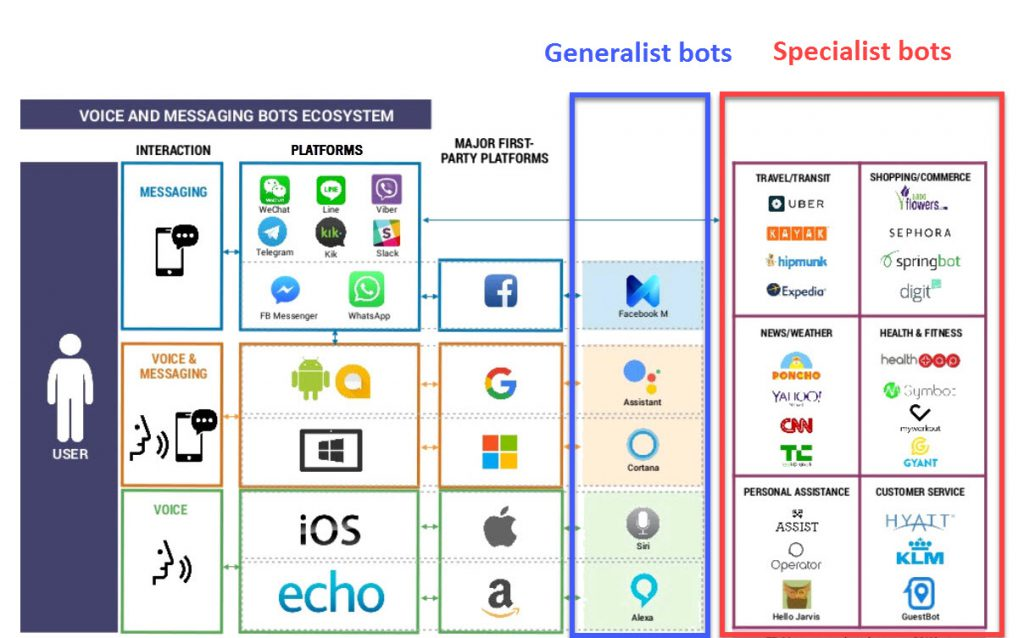
\includegraphics[width=0.9\textwidth]{img/generalist-vs-specialist.jpg}
    \caption{Categorizing Generalized and Specialist Bots \cite{botnerds}}
    \label{fig:ann}
\end{figure}
\\~\\
Now digging in to the generalised bots that how can they be built smart enough to deliver humanly. And then there comes a human characteristic which makes human superior to other beings known as intelligence.

\section{Bots Intelligence}
In order to inject intelligence in to the bots firstly, one should know what is it. So for this reason, a man generated some mathematical models resembling human's brain architecture and tried to train them and made those models to learn by providing some sample information or data. For making the bots intelligent one has to use these models. All existing smart bots use machine learning(ML) and artificial intelligence(AI) techniques to comprehend the language, complex task processing and to figure out the best response. \cite{botnerds}
\\~\\
On basis of the intelligence, bots can be segregated. There are some bots which use and are totally dependent on ML and AI known as "Smart Bots". Those without any AI can be put under the category of "Script Bots" as the just use a script and are totally dumb without it. \cite{botnerds}
\\~\\
Furthermore, AI can also be divided as weak or strong. Weak AI includes pre-defined rules and scopes to make the chatbots work in the right direction. Whereas, strong one is free from such pre-declared rules and is able to learn different behaviours on its own. \cite{CreatingChatbotsToTalk}
\\~\\
Next section explains the high level representation of a conversational agent. 

\section{Chatbots Overview}
Concertedly, there are multiple components that combine to build a chatbot. Whenever there comes any message from the user, it directly passes to language identification module. It varies from simple tag retrieval to more elaborate statistical methods like n-gram models \cite{ngram}. The new message along with the language and potential previous conversation messages retrieved from database, are then pushed to the intent classifier module which identifies the user's conveyed intent. Eventually, a fitting action or a series of actions is produced using the message’s metadata, identified intent and other relevant information from database. Lastly, the action or a sequence is passed to the action handler module as an input and after its execution it generates an appropriate response. \cite{designandimplementation} 
\\~\\
Its diagrammatic overview has been displayed in the Figure \ref{fig:chatbotDiagOverv} below.
\begin{figure}[h]
    \centering
    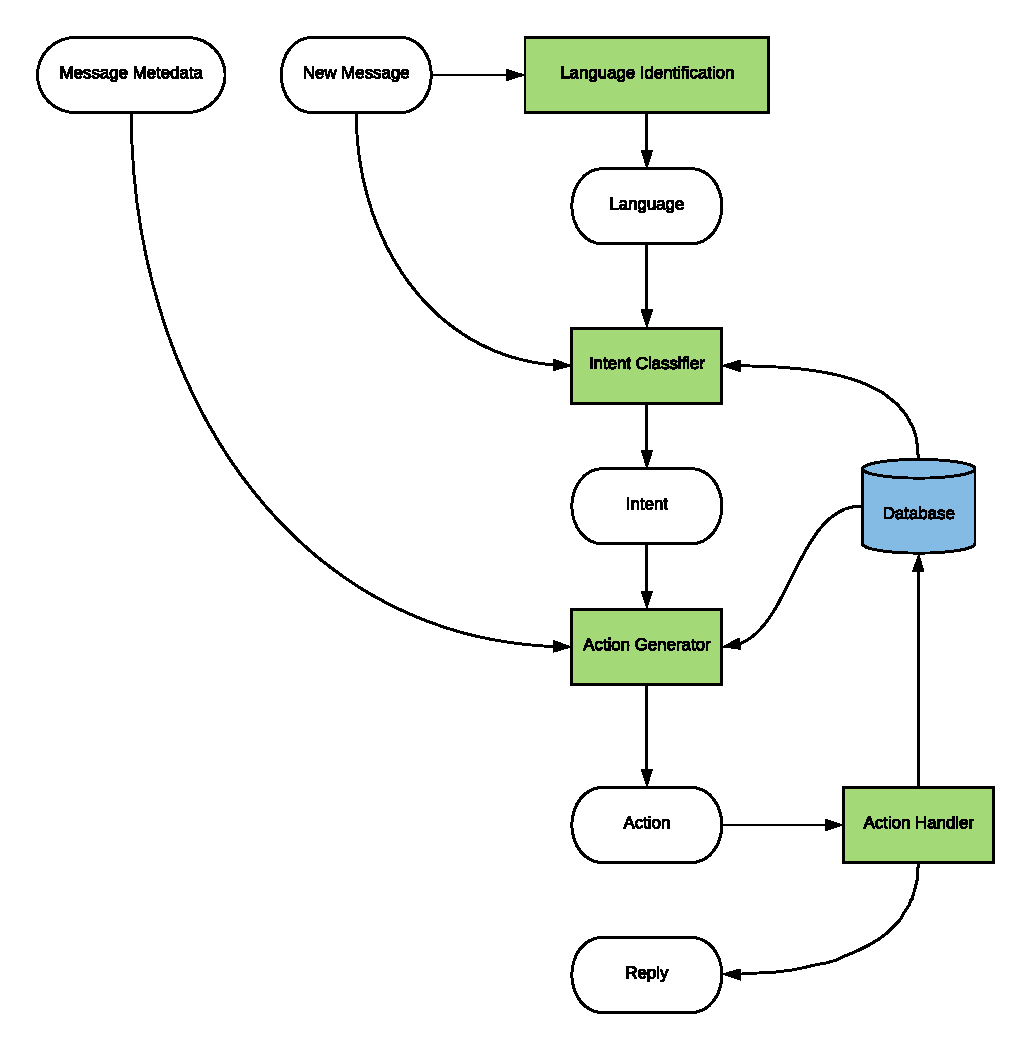
\includegraphics[width=0.9\textwidth]{img/overview.pdf}
    \caption{Chatbots diagrammatic overview \cite{designandimplementation}}
    \label{fig:chatbotDiagOverv}
\end{figure}

\section{Deep Learning Techniques}
In this section some commonly used deep learning will be explained that are used for Natural Language Processing(NLP). When it comes to NLP, Word Embedding and Recurrent Neural Networks are frequently used techniques for deep learning. For Language Identification, it is assumed that utterances can only be written in one language. Furthermore, Intent classification can be done using variety of techniques that vary from Simple Keyword Extraction to Bayesian Inference. Afterwards, response can be generated using retrieval-based and generative-based methods. \cite{designandimplementation}

\subsection{Word Embedding}
Briefly, word embedding technique is used for transforming words in the form of vectors. These mapped vectors can be directly featured in machine learning algorithms. Different methods have already been introduced to exercise this operation. These approaches varies from simple vector count to deep learning methods such as Word2Vec \cite{word2vec}, GloVe \cite{glove} and Skip-gram Model \cite{skipgram}. \cite{designandimplementation}

\subsection{Recurrent Neural Networks}
Recurrent Neural Networks(RNNs) are the neural networks specifically designed for sequenced data. More precisely, such networks work recursively having internal state denoted as \texorpdfstring{C\textsubscript{t}}{C t} at specific time t. Which is passed as an input to the neuron as upcoming time-step and it outputs a value \texorpdfstring{h\textsubscript{t}}{h t} based on \texorpdfstring{C\textsubscript{t}}{C t} at that time-step. But while implementing a simple RNN there comes gradient problems already proven by Pascanu, Mikolov, and Bengio in “Understanding the exploding gradient problem” \cite{gradientproblem}. So to overcome this problem various revised methods have been introduced. According to \cite{designandimplementation} most commonly used ones are mentioned below: 
\begin{itemize}
\item Long Short Term Memory Units \cite{lstm}.
\item Gated Recurrent Units \cite{gru}.
\end{itemize}

\section{Chatbots Tasks and Components}
Chatbots consist of various components and each component is responsible for performing a specific task.

\subsection{Language Identification}
When it comes to larger scale and diversed natural language processing then recognizing a language of a text is a necessary initial step. Some languages contains homographs i.e. Same words with different meanings. It is really a challenging task for an algorithm to understand and grab the correct semantics if language is not known beforehand. \cite{designandimplementation}
\\~\\
It is assumed for this masters thesis that messages will be provided using one language only. Despite of it, there exist methods for inferring different languages in a single document or piece of text and can be found in the document \cite{multilanguagedetection}.

\subsection{Intent Classification}
Another important task that a chatting agent should be able to perform is to classify an intent in the user utterance. It means that a chatbot should be able to detect the purpose of the talk that user is trying to convey. For intent identification, this multi-classification problem is usually solved by labelling the utterances according to the possible user intentions and providing some relative name to them. Furthermore, there exist some techniques to overcome this problem varying from simple keyword extraction to Bayesian inference. These methods are meant to identify the user's request with the help of various messages. Well known LSTM\cite{lstm} networks have been previously used to perform this task due to their high performing and delivering capacity \cite{intentclassificationusinglstm}. \cite{designandimplementation}

\subsection{Knowledge Management}
Knowledge management is directly proportional to intelligence of a chatbot. It means an agent is as much intelligent that how good is it in managing the knowledge provided to it. The task for computers, handling the knowledge progressed significantly in 1980's under the field of "Knowledge Engineering". Methods used for this purpose in the past were consisted of inference tools to shape the facts and evolve new knowledge using first and second order logic. These techniques were used for responding efficiently to ambiguous queries. \cite{designandimplementation}
\\~\\
Knowledge engineering made the functioning easy for conversational bots. As it assists a chatbot to answer a question containing general facts. Apple's Siri and Amazon's Alexa use internal knowledge inference methods to fetch the facts from web and other users resources. \cite{designandimplementation}
\\~\\
In present, Web API calls and optimised requests to the database are extensively used in order to perform this action. Other than that impressive graph-structured ontologies can be used to enhance its performance. \cite{knowledgebase} \cite{designandimplementation}

\subsection{Response Generation}
A conversational bot should have the ability to generate some meaningful response to make the communication effective. So for this purpose it is necessary for a bot to reply coherently according to the context of conversation. This challenging task is executed by following pair of modules:
\begin{itemize}
\item Module to provoke list of competitive responses.
\item Module to select the most relevant reply based on some weighted value or specific metrics.
\end{itemize}
For this sub-challenge, there comes dialogue systems to rescue.

\section{Dialogue Systems}
The importance of human computer interaction has raised drastically in last few years. It is due to its rising potential towards solving daily life problems especially providing aid in commercial challenges. With the advancement of the big data and machine learning, the self functioning virtual assistant is not a dream any more. Based on the applications of conversation companions, the dialogue systems can be divided in to two main categories i.e. Task Oriented Systems and Non-Task Oriented Systems.

\subsection{Task Oriented Systems}
These systems are designed to accomplish a task in some specific domain. The system interprets a message provided by the user, symbolize it to internal state and processes it according to the state of the dialogue. Lastly the final action is performed on it to produce a response in the form of natural language. \cite{surveyondialogsystems}
\\~\\
Mainly natural language understanding is done using statistical models. On the other hand some systems still use human designed pre-defined rules for slot filling and detecting an intent. Which not only results to more time consumption and makes deployment of such system costly, but also restricts the operational domain for the system. To overcome these challenges, deep learning played an important role. Additionally, for extensive representation of state space in pipeline systems, task oriented end-to-end systems have been introduced. \cite{surveyondialogsystems}

\subsubsection*{Pipeline Methods \label{sec:pipelineMethods}}
As mentioned in \cite{surveyondialogsystems} Task oriented systems consisting of pipeline methods inherit following four major components:
\begin{itemize}
\item Natural Language Understanding(NLU) to perceive the semantics of the user utterance.
\item Dialogue state Tracker to supervise the dialogue history and return the recent dialogue state.
\item Policy Learning to predict the upcoming action on the bases of last dialogue state.
\item Natural Language Generation(NLG) for transforming the respective action to the response represented as natural language.
\end{itemize}
Graphical representation of pipeline methods has shown below in the Figure \ref{fig:to}. 
\begin{figure}[h]
    \centering
    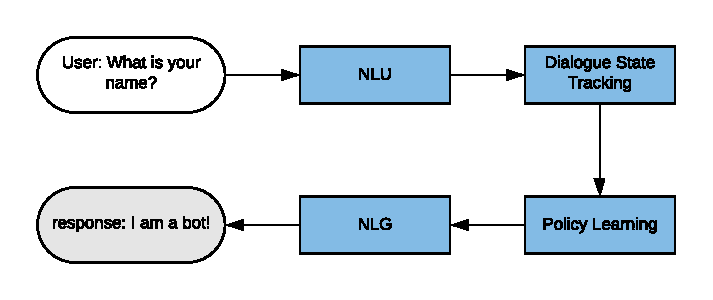
\includegraphics[width=0.9\textwidth]{img/Task_oriented.pdf}
    \caption{Process for Task Oriented Dialog Systems \cite{surveyondialogsystems}}
    \label{fig:to}
\end{figure}
\\~\\
Pipeline based task oriented systems need lot of spoon feeding in particular domain, making them hard to adjust with new domains. In addition to that, the inter-dependency of the components also refrain the system to adapt the new environment. To neglect these challenges end-to-end based task oriented systems have been proposed. \cite{surveyondialogsystems}

\subsubsection*{End-to-End Methods}
Unlike pipeline system, end-to-end system consists of a single module and collaborates with large structured databases. These methods lie under the domain of neural generative models which are discussed below in the section of non-task oriented systems. Many practices have already been made to design a framework for task oriented dialog systems having end-to-end specifications using end-to-end neural generative methodologies. \cite{surveyondialogsystems}

\subsection{Non-Task Oriented Systems}
Main goal of such a system is to communicate with the humans on any topic without restricting it to some specific domain, making them more independent and self sustainable. Applications of such system are entertainment or general conversation with meaningful responses \cite{surveyondialogsystems}.

\subsubsection*{Retrieval-based Methods}
These methods consist of a humongous database containing successive responses. These responses are compared with the information provided by user in form of a message in order to find the best answer for end user. The information provided can usually be a regular expression searching for a specific structures of sentences or any output from machine learning algorithm. This approach benefits the developers by providing a complete control over the responses to prevent any improper answer. \cite{designandimplementation} 
\begin{figure}[h]
    \centering
    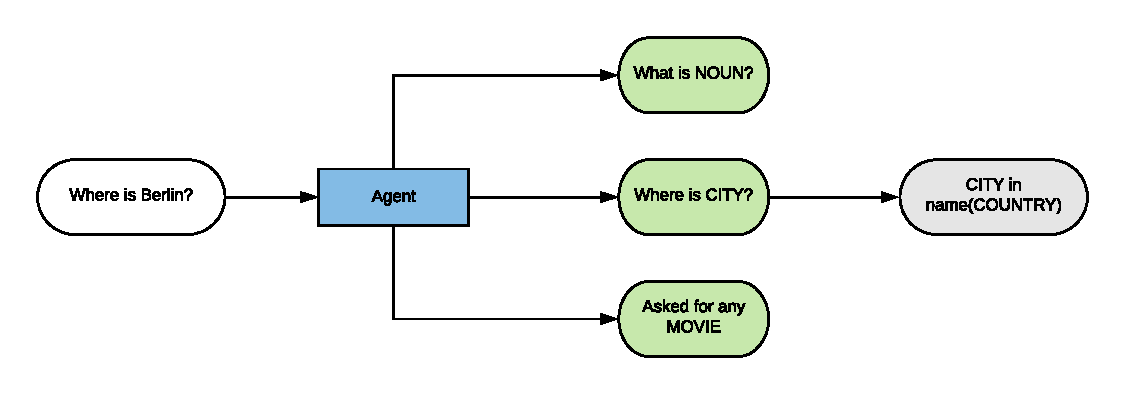
\includegraphics[width=0.9\textwidth]{img/Retrieval_based.pdf}
    \caption{Retrieval-based Methods Example \cite{designandimplementation}}
    \label{fig:rbm}
\end{figure}
\\~\\
The primary and fundamental step to achieve the retrieval-based method is message and response matching. The basic purpose of matching algorithms is to minimize the semantics difference between the responses and the messages. \cite{surveyondialogsystems}

\paragraph*{Single Turn Response Matching}
In this type of matching the only responsible factor for response generation is the message itself. Message context and successive answer are represented as a vector. \cite{surveyondialogsystems}

\paragraph*{Multi Turn Response Matching}
Unlike single turn matching, current utterance along with all past messages are responsible for producing the most suitable response that best matches the overall context of the conversation. \cite{surveyondialogsystems}

\subsubsection*{Generative-based Methods}
Unlike retrieval-based methods, generative-based methods don't need a large database to store pre-generated responses. They are capable of producing a new response based on the user's utterance using generative models. For generating a suitable response it is necessary for the model to be trained enough. Unfortunately, performance of these models is still not sufficient enough to attract the companies due to various restrictions forced by the corporate. \cite{designandimplementation} 

\begin{figure}[h]
    \centering
    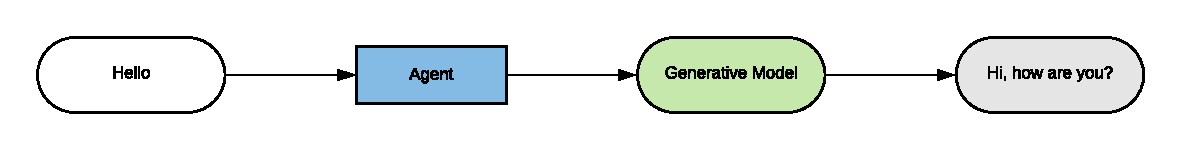
\includegraphics[width=0.9\textwidth]{img/Generative_based.pdf}
    \caption{Generative-based Methods Example \cite{designandimplementation}}
    \label{fig:ann}
\end{figure}
\\~\\
Next section will cover the basis of neural generative models i.e. sequence-to-sequence models. After that there will be explained some research topics underlying these models. 
% \cite{surveyondialogsystems}

\paragraph*{Sequence-to-Sequence Models}
Neural networks are being used by these models in order to symbolize dialog history and to produce useful responses. The systems based on these models doesn't need much knowledge base and pre-defined rules to generate natural language responses. \cite{surveyondialogsystems}

\paragraph*{Dialogue Context}
To keep track of the current state of chatbot and and recent conversation, it is compulsory to take care of the dialogue history and recent user utterances. It helps in understanding the context of dialogues in order to generate appropriate response. Recurrent Neural Networks(RNN) are mainly used for this purpose. \cite{surveyondialogsystems}

\paragraph*{Response Diversity}
To handle response diversity is a challenging task in the systems based on sequence-to-sequence models. As they can provide irrelevant, balanced or completely related answers having some meaning. Inverse Document Frequency(IDF) is mainly used for this purpose. \cite{surveyondialogsystems}

\paragraph*{Topic and Personality}
Topic and personality of the dialogues is another factor to enhance their diversity. By acquiring the fundamental characteristics of dialogues, diversity can be increased and also it leads to gain consistency. \cite{surveyondialogsystems} 

\paragraph*{Knowledge Base}
For making the virtual assistant to perform as humans do there is an essential need of a knowledge base. Not only using outside knowledge base we can cut the informational difference between machines and humans, but can also plant sensibility to artificial conversational agents. \cite{surveyondialogsystems} 

\paragraph*{Interactive Learning}
Eventually the main objective of a dialog system is to be smart enough to do self learning while having an interaction with a user.

\paragraph*{Evaluation}
At the end, the final step is to assess the provoked response quality generated using response generators. Task oriented dialogue systems can be graded using handcrafted methods like rating from the user. Whereas, for non-task oriented dialogue systems its a bit challenging task to evaluate them. METEOR, BLEU and ROGUE are some word overlap metrics to weigh the produced response quality. \cite{surveyondialogsystems}    

\subsubsection*{Hybrid Methods}
Hybrid approaches by combining both above mentioned methodologies have recently been introduced. If response generation fails using retrieval-based methods then it should be produced using generative-based methods. Retrieval based systems gives more accurate results but that could be slow and vague \cite{surveyondialogsystems}. Whereas, neural generative systems have the ability to respond rapidly with the chance of giving useless results \cite{surveyondialogsystems}. So by unifying both of these methods the performance can be enhanced significantly. More study about these methods can be found in \cite{generateifnotretrieve}.

\section{Chatbot Comparison Framework}
On the basis of currently introduced chatbots like Hubot, J.A.R.V.I.S., Pandorabots, Wit.ai etc. the fundamental features vary and can be compared for virtual agents. The key elements are discussed below.

\subsection{Types}
According to \cite{frameworkforunderstandingchatbots} chatting assistants can differ on the basis of their tasks that the are performing. Alertbot is a chatbot that is being used for auto-generating notification for some event occurred. Whereas J.A.R.V.I.S. is a well-known framework for developing artificially intelligent virtual assistants that are capable of rapid self learning and can execute engineering task without any human help. Referring to \cite{softwarebots} chatbot types can be classified as following: 

\subsubsection*{Informative}
Such type of conversational agents are designed to help creators by grabbing required information for some specific task. For example, to produce an alert message for any bug in a program written by some developer. 
% \cite{frameworkforunderstandingchatbots}

\subsubsection*{Collaborative}
These kind of chatbots assist the developers to collaborate and communicate efficiently in order to be more productive. As an example, the collaborative chatbot will alert a developer working on some project, of a chat that is started by some other developers if it involves the one who is working on it and is important for him to be notified. 
% \cite{frameworkforunderstandingchatbots}

\subsubsection*{Automated}
Such chatbots work alongside with the developers to provide aid in tasks accomplishment, having dependencies in one or more projects by detecting the problem caused due to some alteration in a feature. E.g. Auto-generated documentation.
% \cite{frameworkforunderstandingchatbots}

\subsection{Direction}
As mentioned earlier, chatbots differ in the tasks objectives they are performing. On the other hand they function uni-directionally rather than taking the whole conversation in to account. \cite{frameworkforunderstandingchatbots}

\subsubsection*{Input}
Such conversational bots search for some specific keywords or tags pushed by the creator in conversation and fire specific responses based on that keywords or phrases. They are also known as silent bots as they perform their tasks quietly. \cite{frameworkforunderstandingchatbots}

\subsubsection*{Output}
Output chatbots are opposite to input ones. They just need general content or an action to make them operational unlike input bots which require some special keywords to make them trigger any output. Such kind of assistants mostly get activated from some external source and notify about events to a different place. \cite{frameworkforunderstandingchatbots}

\subsubsection*{Bidirectional}
Bidirectional conversational agents work in both directions. They are capable of taking an input and generating an appropriate response accordingly. It can vary from activating just a simple response for some action to real communication. \cite{frameworkforunderstandingchatbots}

\subsection{Guidance}
When it comes to complex chatbots, it is really important to make them function autonomously for their sustainability and practicability.

\subsubsection*{Human Mediated}
These kind of chatbots require human mediation in order to function properly. They can't complete any task on their own. They seek for the relevant information or operational directions from the developer due to which they can not cause much destruction. But if they start to do that then it is very easy for a developer to stop them from further functioning. \cite{frameworkforunderstandingchatbots}

\subsubsection*{Autonomous}
Chatbots which have the ability to perform their tasks on their own and contain all the viable knowledge or having the capability of self learning lie under autonomous agents group. The only problem with such bots is that they can be invasive. \cite{frameworkforunderstandingchatbots}

\subsection{Predictability}
Usually, there is a group of developers responsible of designing any virtual assistant for chatting. With the diverse mindsets of developers there comes uniqueness in specifications and functionalities of a bot. So they can be distinguished on the basis of the genre of tasks they are designed to accomplish. As stated in \cite{frameworkforunderstandingchatbots}, underneath are the following genres:

\subsubsection*{Deterministic}
Chatbots with the deterministic approach perform particularly the same action whenever they observe the similar event or scenario. Such communicating agents involve decision tree to make decisions based on the input provided to them. So it is easier to predict the behaviour of such virtual assistants. 
% \cite{frameworkforunderstandingchatbots}

\subsubsection*{Evolving}
As it is clear from the heading's name that these bots have the ability to evolve themselves. Which means they contain learning element and have the ability to gather knowledge from the past experiences and results. According to which they can regulate their actions. Which results to enhance their performance by making them capable of performing such tasks which were not instructed to them by the developer. But the drawbacks of such agents can't be ignored as they can do self learning and can get out of control while conversation. For example, there was a chatbot for natural language multi-issue bargaining developed by Facebook. Eventually, they had to stop it because it started evolving a language which humans were unable to understand \cite{fbshutdownbot}. 
% \cite{frameworkforunderstandingchatbots}

\subsection{Interactivity}
As no one can deny the fact that it is still a long time to make chatbots act like humans. But the necessity of developing human-like chatbots is rising day by day and lot of research is happening to make chatbots interact as humans do. Although advanced chatbots can have the ability to contain more vocabulary and communicate in a much better way. It helps in enhancing the user experience and promoting chatbots effectiveness. \cite{frameworkforunderstandingchatbots}
\\~\\
As claimed by \cite{frameworkforunderstandingchatbots}, there exist several styles in which chatbots interact with users as mentioned below:

\subsubsection*{Dull}
Chatbots with dull interaction style make conversation using common and repetitive vocabulary and chunks of words. They always use the same welcome message to greet the user without any sense to develop the new meaningful phrase with same semantics. 

\subsubsection*{Alternate Vocabulary}
Such virtual agents consist of a container with multiple equivalent phrases for the same user utterance. They randomly choose the response out of a container for the utterance with same semantics. Which makes these bots superior to dull ones. 
% \cite{frameworkforunderstandingchatbots}

\subsubsection*{Relationship Builder}
Such conversational assistants try to build a good relationship with the developer or end user. Terms used by these chatbots differ from formal to casual and vice versa. They are capable of doing continuous communication. While communicating, they can reach a point to crack a joke for humorous purpose in order to improve the bond and fun experience with the user. 
% \cite{frameworkforunderstandingchatbots}

\subsubsection*{Human-like}
These are the most learning chatbots which use the past chat history for its training in order to become intelligent enough for producing appropriate response for the user query.  
% \cite{frameworkforunderstandingchatbots}

\begin{figure}[h]
    \centering
    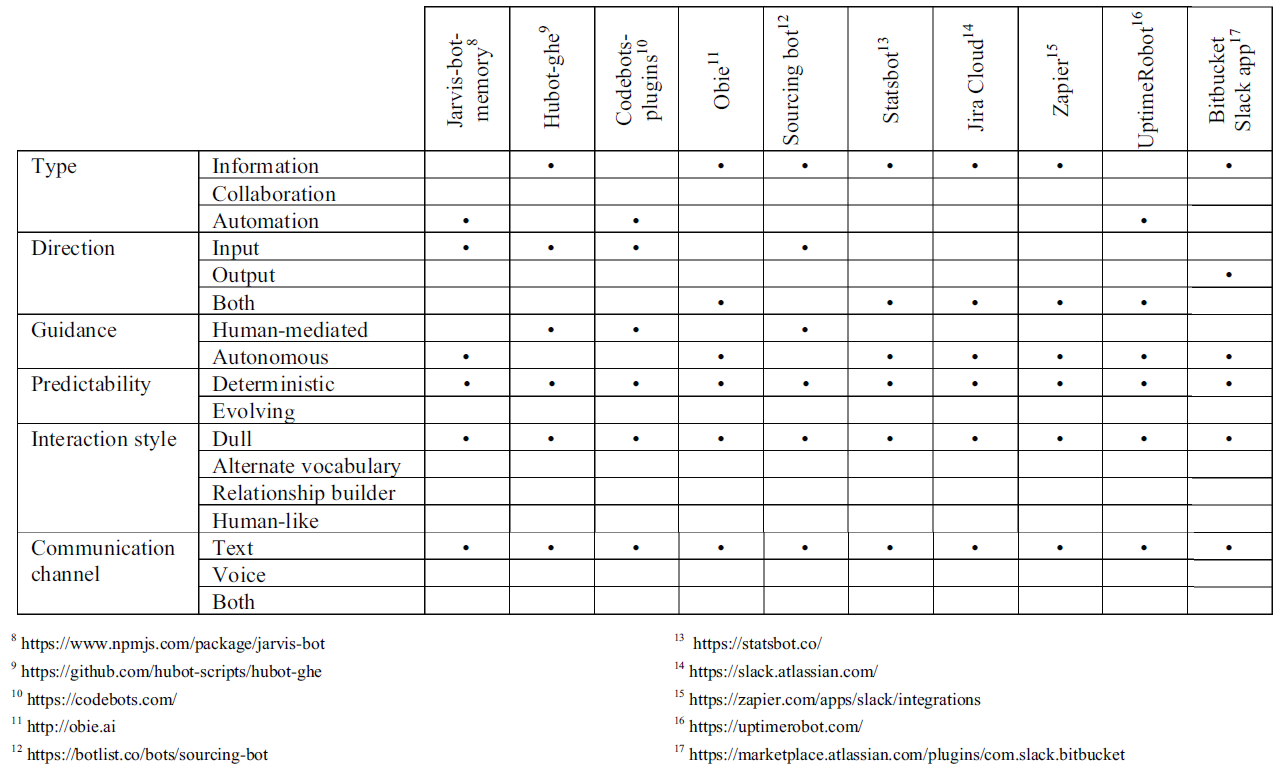
\includegraphics[width=0.9\textwidth]{img/Chatbots_Comparison_Framework.PNG}
    \caption{Comparison framework practiced for software development on selected chatbots. \cite{frameworkforunderstandingchatbots}}
    \label{fig:chatcompfram}
\end{figure}

\subsection{Communication Channel}
There are two types of communication channels that almost all the chatbots are using for communication i.e. messaging platforms for text messages like Slack and speech communication platforms like Alexa. \cite{frameworkforunderstandingchatbots}

\subsubsection*{Text}
These chatbots use text messages for communication. They have an extra advantage as the input and output is in textual form which is easier to understand, store and adapt. It also provides an ease for a developer. \cite{frameworkforunderstandingchatbots}

\subsubsection*{Speech}
Chatbots with voice or speech feature support are more user convenient and provide more realistic and natural mean of communication as they take input using vocals and produce spoken output. Despite of that, they do not implement the facilities which are offered by the ones using text. \cite{frameworkforunderstandingchatbots}

\subsubsection*{Text and Speech}
There also exist such chatbots which have the conversational support using both voice and text channels. They provide the user with an option to configure the way of taking an input and expressing the output. \cite{frameworkforunderstandingchatbots} 

\section{Dialogue Management Systems}
This section covers the role, methods and problems occur while managing dialogue systems. They have been introduced a long time ago under the shadow of systems supporting database queries. One can easily question a computer using natural language or scripted language such as SQL for fetching database information. Dialogue management systems are required for complex utterances from the user in order to deliver decent responses.

\subsection{Role}
Systems designed for dialogue management are meant to imitate conversation processing. Shaping a dialog from any source such as speech, text or any other approach is an essential step for making a dialogue manageable. If there occurs a system failure then communication must not have a full stop. The dialogue manager should be capable of catching a reason of failure and endorsing a dialogue recovery. \cite{dialoguemanagementsystems}

\subsection{Discourse Characteristics}
Conversation or debate between humans is not something that can be easily understandable by computers. It comprises of many complexities. But while having a dialogue between machines and humans, one can make a communication using simpler language but still a person expects that system should hold various features as claimed by \cite{dialoguemanagementsystems} are stated below: 
\begin{itemize}
\item \textbf{General Structure:} Dialogue consists of opening, body and closing. User can handle the dialogue at its opening and closing point. Whereas, management system controls the body part of a dialogue.
\item \textbf{Combined Initiative:} Usually user holds most of the control over a dialogue. Then there comes a system to take over the control for diminishing the misconception, if there occurs any. And this task of management system is mostly gets accomplished by verification of information provided, eliminating the confusion or by restraining the user's reply. 
\item \textbf{Over Gossipy:} It is in a humans nature to provide the extra useful information to others which is not even asked explicitly at that moment. Same goes with dialog management systems that they should be able to do it.
\item \textbf{Contextual Sensation:} System must be capable of sensing and understanding the semantics and context of the dialogue.
\item \textbf{Error Restoration:} If there happens any error or misconception leading to dialog failure then system should be able to restore it and not letting the conversation to stop. 
\end{itemize}

\subsection{Modelling Dialogue Challenges}
Following are some facts and realities of a dialogue stated in \cite{dialoguemanagementsystems}, which can not be ignored and must be taken into account while modelling a dialogue: 
\begin{itemize}
\item \textbf{Turn Switching:} Handling the switching of turns between user and agent or between two agents. 
% \cite{dialoguemanagementsystems}
\item \textbf{Conversational Fillers:} While communicating humans usually use interjections like aah!, nah!, yep! and oops!. Such words are known as fillers as they don't contain any meaning but are useful to increase the cohesiveness and convey the intentions of the user.  
% \cite{dialoguemanagementsystems} 
\item \textbf{Ellipsis:} Ellipsis are words omitted by humans during conversation but can be understood using context of previous discourse. So it is another factor that should be taken under consideration while modelling a dialogue. Otherwise, system will not be able to deliver smartly like humans do. 
% \cite{dialoguemanagementsystems}
\item \textbf{Indirectness:} It involves the communication in which literal meaning of an utterance conveys wrong meaning. But by using the intellectual capabilities, participants can interpret the correct semantics.
% \cite{dialoguemanagementsystems}
\item \textbf{Adjacent Dependency:} It occurs when two participants are communicating and one asks a question but second participant instead of replying to it, posts another related question. Now its a first one turns to respond to the question raised by the second participant in order to get answer of his firstly asked question. 
% \cite{dialoguemanagementsystems}
\item \textbf{Anaphoric and Cataphoric Reference:} Anaphoric reference is used to get the meaning of the recent word by referring to a term used previously in the text. In contrary, cataphoric refers to a word used afterwards in the text to understand the meaning of recently mentioned word. For example, last/next, now/then, I/you etc.
% \cite{dialoguemanagementsystems}
\end{itemize}

\subsection{Dialogue Classification}
Classify the dialogues is not an easy task to perform. Specially when it comes to taxonomize them on the basis of their features. The classification proposed by Dahlbäck in 1995 is based upon the tasks executed by Rubin in 1980 and Clark in 1985. According to them, dialogues can be classified under four dimensions as mentioned in \cite{dialoguemanagementsystems} are:  
\begin{itemize}
\item \textbf{Agent type:} It includes humans and computers with great impact on the language used to communicate. It has been noticed that while having a conversation with virtual agents, humans use utterances conciser, simpler and shorter linguistics.
\item \textbf{Communication Channel:} It underlines many distinguishing  features but the most important one out of them is the method used for communication i.e. spoken or written. Other factors involve transmission styles. 
\item \textbf{Type of Task:} It is another factor having huge impact on the structure of a dialogue. Additionally, task context also have a great affect. Another important aspect having strong impression on dialogue's structure is number of tasks performed by a single dialogue.      
\item \textbf{Mutual Knowledge:} Knowledge shared among the dialogue contestants also has an influence on language which can not be ignored. There exist three ways to deliver the information between dialogue participants.
\begin{enumerate}
    \item Perception between speaker and listener.
    \item Lingual between both.
    \item Cultural knowledge.
\end{enumerate} 
\end{itemize}

\section{Dialogue Management Techniques}
A good dialogue management tool must include two necessary elements concerning interaction between a user and a bot. The first one is referred to as conversation background or history for correctly determining the context of a dialogue. Whereas, second important element is an interaction model designed to govern the system's approach for handling schema of conversation. \cite{dialoguemanagementsystems}
\\~\\
There exist numerous methods to artifact systems for dialogue management. But each system should include some basic components as shown in Figure \ref{fig:gsls}. Input is provided to the system as a text or interpretative speech which is further processed by natural language understanding component to infer the context and semantics. Dialogue manager is mutually connected with all components to deduce all related and meaningful related information, remove confusions and conflicts. Dialog manager's output is being used by response generation unit in order to produce response in the form of natural language or any other suitable representation may be outlined as a text to sense visually. If it is generated as natural language then there comes a speech synthesizer to performs its task by reading it out loud for the user. \cite{dialoguemanagementsystems} 
\begin{figure}[h]
    \centering
    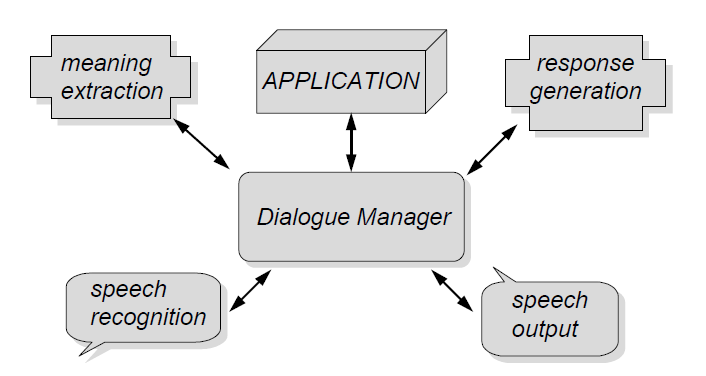
\includegraphics[width=0.9\textwidth]{img/Generic_Spoken_Language_System.PNG}
    \caption{Generic Spoken Language Systems \cite{dialoguemanagementsystems}}
    \label{fig:gsls}
\end{figure}
\\~\\
As Figure \ref{fig:gsls} depicts just an overview of spoken dialogue systems. For more illustrative and detailed demonstration of different units along with the tasks that they are responsible for, just have a look at Figure \ref{fig:dsdm} below.
\begin{figure}[h]
    \centering
    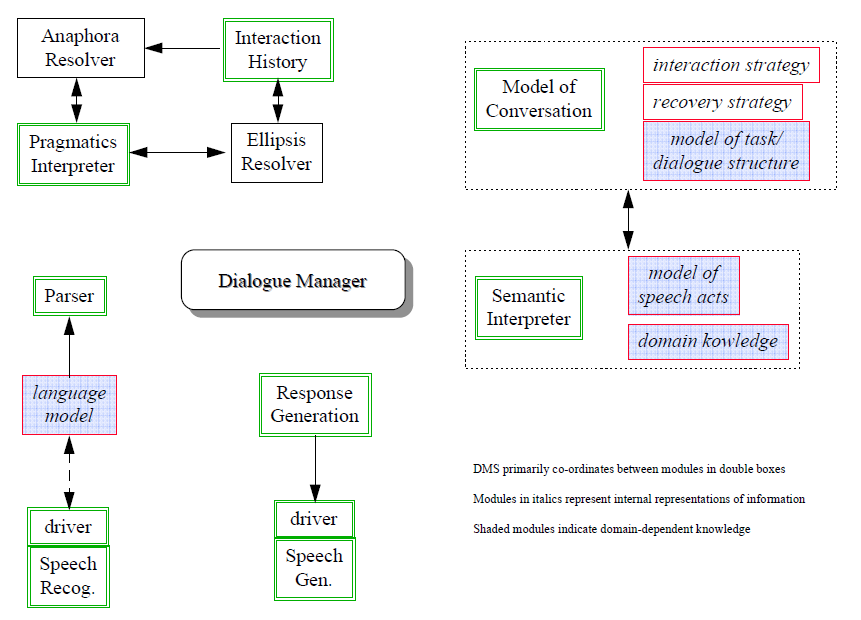
\includegraphics[width=0.9\textwidth]{img/Detailed_Spoken_Dialogue_Manager.PNG}
    \caption{Detailed Spoken Dialogue Manager along with Key Components \cite{dialoguemanagementsystems}}
    \label{fig:dsdm}
\end{figure}

\subsection{Grammars for Dialogue} 
It is the most common initial method out of all the firstly introduced methods. It uses directed grammar from sequential sentences for dialogue description. Usually the grammar describes the architecture of whole communication. According to \cite{dialoguemanagementsystems}, following is the most commonly used approach for this purpose. 
% \cite{dialoguemanagementsystems}

\subsubsection*{Finite State Machines and Graphs}
Finite state models and graphical representations are the simplest methods used for managing a dialogue. Best scenario to get full benefit out of these is, when the structure of the dialogue resembles the structure of the task. Interlinked nodes join to build a graph which minimizes the user choice for selections at that very moment. And with each leading response, the state changes to another node. Like other techniques, it also has advantages along with some disadvantages. As a positive stance, the system has the overall control over the communication by limiting the user choices. On the other hand they also lack the flexibility  to be adapted by some different task and domain. \cite{dialoguemanagementsystems} 
\\~\\
To overcome the flexibility issue, there comes plan based approaches to rescue.

\subsection{Plan-based Methods}
When it comes to complexity, these methods are considered to be more complex for dialogue designing as compared to dialogue grammars approaches. These methods are goal specific like humans as they communicate to achieve different objectives. These methods are used to architect these goals and sub-goals for a task or dialogue. \cite{dialoguemanagementsystems}
\\~\\
Stated below is an application of a plan-based method taken from \cite{dialoguemanagementsystems}.

\subsubsection*{Conversational Games Theory}
It is a well known pattern to develop a dialogue architecture at mass level. In addition to that, it can also be beneficial to design a task oriented dialogue among humans and a computer.  Both grammars from the dialogue and pattern-based approaches are involved in its development. There exists a set of rules or we can call them turns for each game. Which includes the response for some question. So hypothetically, there exists dialogues and each dialogue is responsible to complete some small task. Which collectively results in accomplishment of the main task. And each dialogue is responsible for performing some transactions which represents a sub-task. Whereas, every transaction represents a game associated to some conversation. 
% \cite{dialoguemanagementsystems}

\subsection{Collaborative Methods}
Humans collaborate with each other in order to develop some understanding among them. The main idea behind these methods is to involve both of the participants for a dialogue to get the sense of mutual understanding. Collaborative techniques have main focus on the incentive of the dialogue unlike, pattern-based approaches with having task structure as a main target. Additionally, these methods also try to grasp the dialogue structure. Which means these approaches have the ability for catching general dialogue properties. \cite{dialoguemanagementsystems}

\section{Dialogue Management Systems: Challenges}
There exist two major concerns for a dialogue management system. First one includes the coding strategy for design and structure of a system. Secondly, the recovery technique in order to overcome a particular error is also a challenging task.

\subsection{Coding Strategies}
Strategies used for coding purpose are most often independent of a dialogue structure. They are usually used to design conversation using deterministic approach i.e. finite state machine, or non-deterministic approach i.e. statistical model. Coding scheme and modelling strategy are responsible for the amount of information that can be delivered using a dialogue. There are different types of techniques that can be useful under different circumstances. But the basic need is to understand the user point of view from the utterance which in fact is a challenging task. And for better understanding of a user intention, support can be taken from the context. So for this purpose, a linguistic philosopher Austin in 1962 initiated the research which was later named as Speech Acts Theory after the contributions by Searle in 1969. \cite{dialoguemanagementsystems}  

\subsubsection*{Speech Acts}
Austin initiated it after noticing that some user utterances are not only the statements but can be an order to perform some action. He demonstrated following two sentences to make it more understandable:
\begin{enumerate}
    \item “I bet you six pence it will rain tomorrow”
    \item “I name this ship the Queen Elizabeth”
\end{enumerate} 
These statements can not only be judged as true or false. So he classified such statements as Performative Statements. Whereas, those statements that can be examined using true/false flags were named as Constative Statements.
\\~\\
Later, the classification proposed by Austin was proven wrong. As both types mentioned before can be put under the shadow of illocutionary acts. Illocutionary reflects the true purpose of the statement that can be an offering, promise or a warning. This illocutionary act was named as "Speech Act". Which demonstrates the true view point of the user utterance. 
\\~\\
With its applications, a problem was raised when identified act doesn't match intended user act. To overcome the problem, the identification of perlocutionary act is important. For example, "It is cold in here" seems not to be a statement but a request to turn on the heat or any other related appeal. So, Searle in 1975 declared it as another type of speech act Indirect Speech Act(ISA). But it made the automatic labelling a real problematic task due to the uncertainty of the utterance that if it should be considered literal or interpreted. 
\\~\\
Furthermore, Brown and Yule in 1983, proposed another problem with speech acts while applying them to user utterances. Speech acts need one-to-one mapping between user utterance and an act. But there can be a scenario where multiple user utterances are responsible to complete a speech act or multiple speech acts can be performed with the help of a single utterance.
\\~\\
Considering above mentioned problems with speech acts, Bunt in 1989 came up with another approach to succeed speech acts and that was Dialogue Interpretation Theory(DIT). According to this theory, the dialogues can be classified under two categories: task oriented for controlling a dialogue and proposed content integration. \cite{dialoguemanagementsystems}

\subsubsection*{Dialogue Structure}
A dialogue having independent domain can add some structure to a dialogue while getting converted to dependent morphology. But the structure added is limited to the general acts. As mentioned above, conversational game theory adds a dialogue structure on top of speech act.
\\~\\
Another methodology of adding a structure to a dialogue was introduced by Alexandersson in 1996. It takes a collection of dialogues followed by dialogue acts to produce intentional structure for itself. Which means a dialogue is divided in to goals and sub-goals to gain a structure with some hierarchy. This process can be completed using following three steps as stated by \cite{dialoguemanagementsystems}\cite{automaticacquisition}: 
\begin{enumerate}
    \item Acts in a collection are traversed to convert them to domain independent from dependent hierarchy.
    \item Encapsulate dialogue sequences in different classes. Which are responsible for some functionality or representing a dialogue phase.
    \item Auto-production of context-free-grammar using Bayesian Model.
\end{enumerate} 

\subsection{Error Recovery}
There is a high risk of task failure but it should be made sure that a dialogue must go on. It should be highly prioritize that the dialogue manager must be able to catch the error and handle it properly. Which means it should be able to recover from such faulty situations. The bugs can vary from speech recognition to inaccurate semantic analysis of user's utterance. For this purpose, it is necessary for a manager to encounter it correctly and undergoes some appropriate strategy. So, the taken action may differ depending upon the scenario. It must follow recursive pattern to detect errors that occurred while solving the old one. \cite{dialoguemanagementsystems}
\\~\\
While handling speech recognition, mainly following three types of errors are generated as referred by \cite{communicationaldeviation}\cite{pragmaticinterpretation}: 
\begin{itemize}
\item \textbf{Uncertainty:} It occurs when there is low confidence for a speech input.
\item \textbf{Inconsistency:} It refers to misconception or misunderstanding. Which means the input speech holds high confidence value but opposes the former conversation.       
\item \textbf{Ambiguity:} It occurs when system gets confused between more than one high confidence values for a speech input.
\end{itemize} 
\\~\\
Luperfoy proposed the following four steps recovery method in 1996 as stated by \cite{tutoringversustraining}\cite{dialoguemanagementsystems}: 
\begin{itemize}
\item \textbf{Detection:} Error detection is a challenging task and can also be user dependent to inform the system about it.
\item \textbf{Diagnosis:} It includes error classification.       
\item \textbf{Selecting Repair Plan:} It depends upon the diagnosed error class.
\item \textbf{Executing Interactive Plan:} Selected recovery plan should be executed in an interactive manner to fairly deal with the errors produced by the plan executed.
\end{itemize}

\section{Dialogue Management Systems: Evaluation Methods}
Once the dialogue management system(DMS) is developed and ready to be launched, it must be undergone through some evaluation techniques. It never has been an easy task to perform evaluation for the dialogue systems. Usually its complexity depends upon the criteria of what to evaluate and how to evaluate. In addition to that, assessment is also dependent on different features. The ability of a system to auto-recover itself in case of any error is known as robustness. It should be assessed beforehand during implementation of a system. The other essential thing to evaluate is effectiveness of a system that is, how effective, acceptable and friendly a system is for managing a dialogue. According to \cite{dialoguemanagementsystems}, there are two of the following methods already being introduced i.e. Quantitative and Qualitative Approaches.

\subsection{Qualitative Methods}
It can be inferred from the name that such methods are used to evaluate the quality of a DMS. These methods involve users to get the mission accomplished. So users opinions play major role in order to make assessment decisions for a system. 
\\~\\
For carrying it out, once the users have adopted and utilized a system, they are provided with a questionnaire to fill or an interview can be conducted for them with different questions regarding performance of a system. Which also includes the questions about performance, natural behavior, user friendliness of the system and how well it performed under certain circumstances. It also varies from person to person that some persons respond positively whilst others can provide negative impressions. Even though the system is same based upon different user preferences. So, it is better to make a user well familiar with a system first and then ask him/her to give an opinion.
\\~\\
Some interviews had been conducted by Dybkjaer in 1995 after making the users familiar with a system which can be found in \cite{qualitativeevaluation}.

\subsection{Quantitative Methods}
In order to assess a DMS quantitatively, already two techniques have been introduced so far i.e. black box and glass box. 

\subsubsection*{Black Box Testing}
It is based upon the input and the respective output without caring about the design and other internal structure of a system. It is just an outer level or top level evaluation and can be performed by the end user.

\subsubsection*{Glass Box Testing}
In this type of assessment, system's internal individual components can be evaluated. And for this purpose, it is necessary for a developer to have the data from the past so that the current output of a component can be compared with the previous one. Such comparison can provide one with the information about accuracy of the the DMS. Such testing can't be performed using black box technique as there is no trustful data available for comparing a dialogue. \cite{dialoguemanagementsystems}

\subsection{Cross-systems Comparison}
In addition to above mentioned evaluation techniques, there also exist some other methodologies to evaluate the dialogue management systems such as objective performance evaluation. It is recommended to perform objective evaluation for the dialogue to make its performance comparable with other management systems. Also in present era, there are several state of the art chatbots available like IBM Watson etc. One can also easily evaluate self created DMS by doing comparison after designing same dialogue on any other state of the art virtual assistants.

\subsection{Evaluation Metrics}
Also there are following evaluation metrics used to quantify the performance of a chatbot according to \cite{differentMeasurementsMetrics}:
\begin{itemize}
\item Dialogue efficiency metrics in terms of matching type.
\item Dialogue quality metrics based on response type.
\item Users' satisfaction assessment metrics.
\end{itemize}
\\~\\
Next chapter illustrates the system architecture and overview of the chatbot named as "Frankenbot" along with its capabilities.


    \chapter{Frankenbot: System Overview and Capabilities \label{cha:chapter3}}
In this chapter, you can find all the details about the implementation of a framework utilized to design the bot known as "Frankenbot". Additionally, there is a complete description of the system's architecture, features, and abilities of the framework. 
% Lastly, the chapter will be closed by highlighting future goals along with the conclusion.
\\~\\
If you are wondering where does the name "Frankenbot" comes from and why? So firstly, let me remove your confusion. It is derived from the fictional character known as "Frankenstein". It was first introduced in a novel written by Marry Shelley in 1818. Later on, after getting the hype it was promoted using different media sources like films, T.V. series, and also adopted by the gaming industry. Furthermore, the most well-known edition for its representation was the movie renowned by its original name released in 1931 \cite{frankenstein}. In this movie, Frankenstein was pictured as a haunted scientist who loved to dig the graves of humans and used to create new living beings by reassembling their expired body parts \cite{frankensteinmovie}. Likewise, Frankenbot is also a composition of different components as explained below in detail.

\section{Why Frankenbot?}
Currently, there are many states of the art dialogue frameworks available in the market like Rasa, Plato, and IBM Watson. But the question rises why Frankenbot and what makes it different from other well-known frameworks. There exist the following challenges that still need to be addressed.
\\~\\
Firstly, the question raises in mind that, is it possible to design a chatbot that is composed of several small chatbots? Secondly, what if the answer is yes? And one can build a giant chatbot using tiny virtual assistants then how can be the components and modules of a chatbot can be reused? Thirdly, how to make a platform-independent chatbot? In addition to that, another problem is the re-usability of a dialogue between different chatbots. Furthermore, there is another complication that can not be ignored is the rigidity handling for a chatbot. This proposes to inject the flexibility to a chatbot so that it can understand the dialogue consisting of multiple topics without displaying any alert message like "You are currently in the middle of the current dialogue. Are you sure to abort it?". Lastly, the biggest challenge is to design a chatbot that is capable of staying on the topic. This means it should be able to save the current dialogue state for each user instead of just responding with an answer that matches the user utterance irrespective of the current context in the conversation. 
\\~\\
For the above-mentioned challenges, there comes the Frankenbot to rescue and address them well. Additionally, the research completed under this master's thesis is an important step towards integrating different technologies. These technologies could include statistical dialogue managers, question answering, and slot-filler. The product implemented in this study provides the preparatory steps for it.

\section{Frankenbot: Experimental Chatbot}
The main idea behind the development of Frankenbot is to attest to the study of the modular framework implemented in this master's thesis. 
% An experimental chatbot named Frankenbot is designed to evaluate the research that happened under the shadow of this research. 
\subsection{Domain}
The demo chatbot has been designed using entertainment mechanism so that the participants do not lose interest during communication. For this purpose, a detective conversational agent was designed to solve a robbery case. The task assigned to Frankenbot was to ask the user different questions to come up with a decision whether a user answering to those questions is a culprit or not. Whereas, it has been expected from a user to answer the questions or talk generally about the corona virus and its stats, humor, gossips, and other related questions about bot's profile.

\subsection{Design}
Frankenbot has been designed to handle the answers for the questions thrown by it to the users. Secondly, it also has to respond efficiently in case of general conversation. To cope up with these challenging situations, it is provided with two modules. One module for detective dialogue and the other for general conversation. Both modules are implemented using a dialogue tree. Each dialogue tree is composed of interrelated child nodes. And all nodes collectively forming a tree are set to be responsible for containing all the relevant information about the specific module, intents available, and corresponding responses. 

\subsection{Training for NLU \label{sec:expchatbot}}
RASA NLU component has been adopted for the training of Frankenbot to understand the messages well. Additionally, it has been also used for detecting intent and entities in user utterances along with their respective confidence values.  It has been discussed thoroughly under Section \ref{subsec:rasanlu}.  
\\~\\
The detective model has been trained using 115 examples including 6 distinct intents ('\#affirm', '\#bye', '\#robbery\_time\_info', '\#purchasing', '\#greet', '\#negation'). Whereas, the general talk model has been trained by means of 205 statements including 9 distinct intents ('\#gossip', '\#psychology', '\#humor', '\#emotion', '\#coronaStats', '\#botFood', '\#general\_talk', '\#botProfile', '\#corona'). The json data provided for training can be found in Appendix \ref{appen:traindatastats}.

\subsection{Response Generation}
Lastly, the response is generated based on the detected intent with the highest confidence for a user utterance among all the available modules. Moreover, Frankenbot also checks for the current dialogue state and considers different parameters like the last active module and node for each user before responding. And for each intent, there exists a list of responses. And a response gets selected based on the mode assigned to it which can be either random or sequential.  

\section{Frankenbot as Concept}
This section highlights the theoretical functioning of the Frankenbot. Starting from the web-based interface designed for the users to provide input in the form of a text message. This input is passed to the chatbot by making simple get request using Web API. Once it is available to the chatbot for further processing then actual operation gets started.
\\~\\
Initially, the message is passed to a dialogue manager along with the session information and current dialogue state for a user. The dialogue manager holds the complete dialogue structure in the form of the dialogue trees. The number of dialogue trees represents the number of modules contained within a dialogue manager. Furthermore, each dialogue tree is composed of the tree nodes containing the modular information about the specific sub-state of a dialogue along with the intents and comparative responses.
\\~\\
Furthermore, a dialogue manager tries to find out the intent with the highest confidence value for the user utterance. For this purpose, all nodes of available dialogues trees are traversed. Each module contains a separate trained RASA NLU model and intent detection for response generation. A user utterance is processed through all of the generated NLU models to find out the intent and entities for input including the confidence values assigned to them. Later on, this information gets shared with a dialogue manager. It is responsible to keep a check for the highest activation value out of all the intents present in all modules. Additionally, it also keeps track of the module which includes the most confident intent. It also updates the node's activation information about the specific sub-state of a dialogue.
\\~\\
In the end, this information is delivered to a bot to generate a response based on the most confident intent and current state of dialogue for a user. Which is passed to the client as a response to an initial get request made using Web API by a user.
\\~\\
Session information for each user also gets stored along with the last active dialogue state for that specific user. Additionally, context variables are saved to make the response and dialogue more humanly.

\section{Frankenbot: Approach}
The Frankenbot is a chatbot composed of multiple chatbots. The design composes modules that work together to form a chatbot. General graphical representation is shown in Figure \ref{fig:frankOver}. 
\begin{figure}[h]
    \centering
    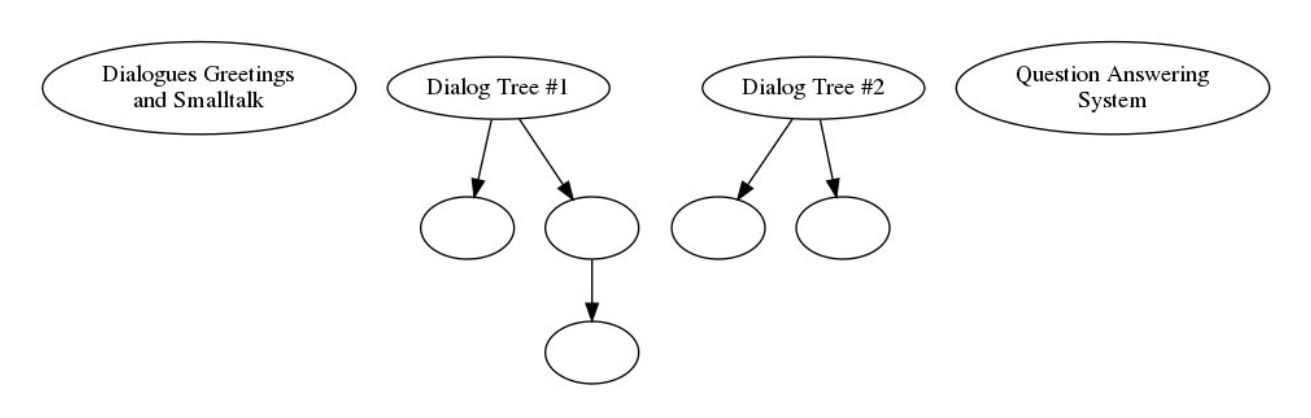
\includegraphics[width=0.9\textwidth]{img/Frankenbot_Overview.PNG}
    \caption{Frankenbot Overview}
    \label{fig:frankOver}
\end{figure}
\\~\\
As displayed, the example is composed of two modules: (i) "Dialogues Greetings and Small Talk" and (ii) "Question Answering System". And each module includes a dialogue tree demonstrating a complete dialogue structure for the respective module. So, "Dialogue Tree #1" belongs to the greetings module, and "Dialogue Tree #2" is linked with the Q\&A module. The module and dialogue tree has been explained in the section below.

\subsection{Module}
A module can provide the answer to a user's utterance. Therefore it requires an activation function Z that maps the current user utterance and the system state to a real number.
\begin{align*}
 Z: utterance, state \rightarrow R
\end{align*} 
For every user utterance, the dialogue manager calls all activation functions and chooses the model with the highest activation function. This module can then generate the answer. The module itself can be anything. It can be a classical intent-based system. Other systems are also possible. Some common examples of the modules are as follows:
\begin{itemize}
\item Bag of request/response pairs \cite{rrpairs}.
\item Waterfall Dialogue \cite{waterfallDial}.       
\item Slot-filler Dialogue \cite{slotfillerDial}.
\item Dialogue tree \cite{dialogTree}.
\item Question and Answering Dialogue \cite{q&aDialog}.
\item Knowledge Graph \cite{knowlGraph}.
\end{itemize}
\\~\\
As a theory, a module can be more than a dialogue tree. Other systems (question answering, neural systems, etc.) can also fit in this framework, as long as they implement an activation function but it still needs to be tested. 
\\~\\
The classic slot-filler/single dialogue tree-based architecture is a basic possible module of the Frankenbot. Therefore the Frankenbot is at least as powerful as the slot-filler.

\subsubsection*{Traditional Dialogue Tree}
One of the data structures used to represent a dialogue is known as a dialogue or conversation tree. Usually, they consist of some sort of data stored in the hierarchical nodes. These nodes are also used to demonstrate the current state of the dialogue by pointing to the current node which has been processed lately. Furthermore, there exist to and fro relations between all the nodes. So this approach acts more likely as Simple Directed Graphs \footnote{\url{https://en.wikipedia.org/wiki/Directed\_graph}}. Just, for example, consider a dialogue with two dialogue sub-trees as shown in Figure \ref{fig:modArch}. In a traditional system we need to model:
\begin{itemize}
\item The transitions from the root node to the sub-tree.
\item The transitions inside each sub-tree.       
\item The transitions from each node to the root node(dashed lines: “I want to cancel this dialogue”).
\item To enable transitions between the sub-trees they would need to be modeled explicitly. In the example, this is omitted due to the complexity of the graph. Also, it is not possible to jump directly to the "subtree #2" while being currently somewhere in "subtree #1". Switching is only possible by following the available path to it.
\end{itemize} 

\begin{figure}[!h]
    \centering
    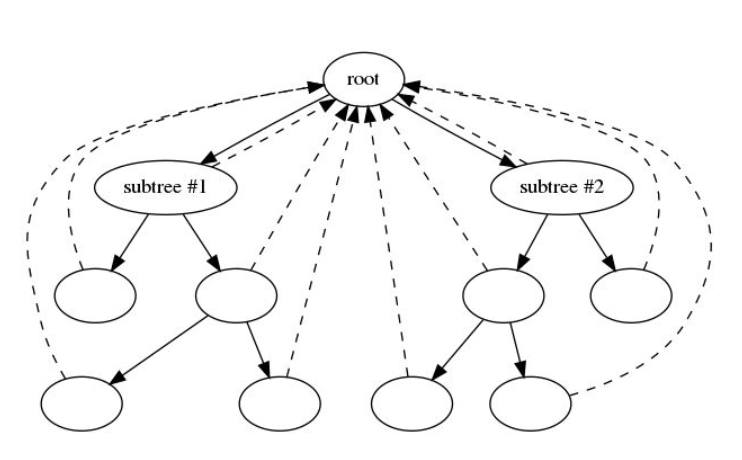
\includegraphics[width=0.9\textwidth]{img/Modular_Architecture.PNG}
    \caption{Traditional dialogue tree containing two sub-trees.}
    \label{fig:modArch}
\end{figure}


\subsection{Modular Architecture}
There are various benefits for using modular architecture. 
% \subsubsection*{Modular Architecture's Characteristics}
Utilizing this architecture many features can be unlocked. Usability and performance can also be enhanced as mentioned below:

\paragraph*{Simpler but robust dialogue trees\label{par:simplerTree}}
The same dialogue as mentioned above but with the Frankenbot's framework modular architecture is shown in Figure \ref{fig:modArch2}. As you can notice the dialogue tree is less complicated and more powerful.
\begin{itemize}
\item Jump back to the root node is not necessary.
\item Switching between trees is possible without explicit modeling.       
\item Going back after switching is possible without explicit modeling.
\end{itemize}

\begin{figure}[!h]
    \centering
    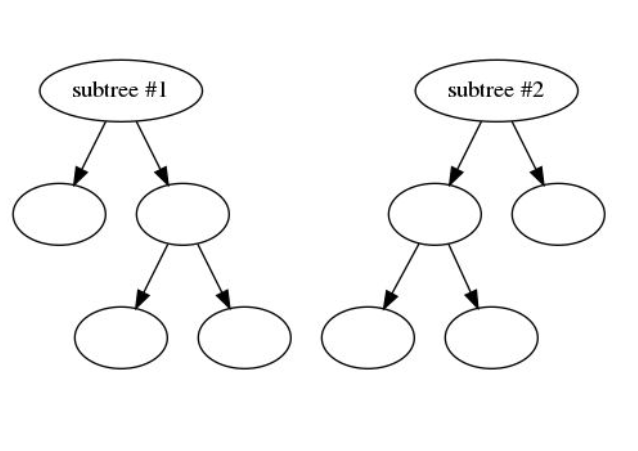
\includegraphics[width=0.9\textwidth]{img/Modular_Architecture_2.PNG}
    \caption{Dialogue with two sub-trees using Modular Architecture}
    \label{fig:modArch2}
\end{figure}

\paragraph*{Unification of Smaller Chatbots}
In this framework, all modules remain independent of each other. They are not tied together. Using this architecture the complexity of larger chatbots can be declined by dividing them into smaller liberated bots. In other words, the complexity of larger chatbots could be reached using the divide and conquer rule. This modular architecture provides a better framework for larger chatbots to grow. It also provides more customization options to a bot as one can easily add and remove any module from any bot at any time without caring for its dependencies.

\paragraph*{Modules Usability}
Modules can be reused within the same chatbot or different chatbots:

\begin{itemize}
\item \textbf{Usability within a Chatbot:} Modules can be reused within a chatbot. Just consider an example as shown in Figure \ref{fig:modReus2}. 
\\~\\
Imagine a chatbot from the smartphone support domain. Two dialogues require how to find out the model of the smartphone. The smartphone model will be stored as an environment variable. Transitions with a diamond tail are only possible when this environment variable is set. The transition with the dashed line does not leave the current node. It only activates the node in the next tree.
\begin{figure}[!h]
    \centering
    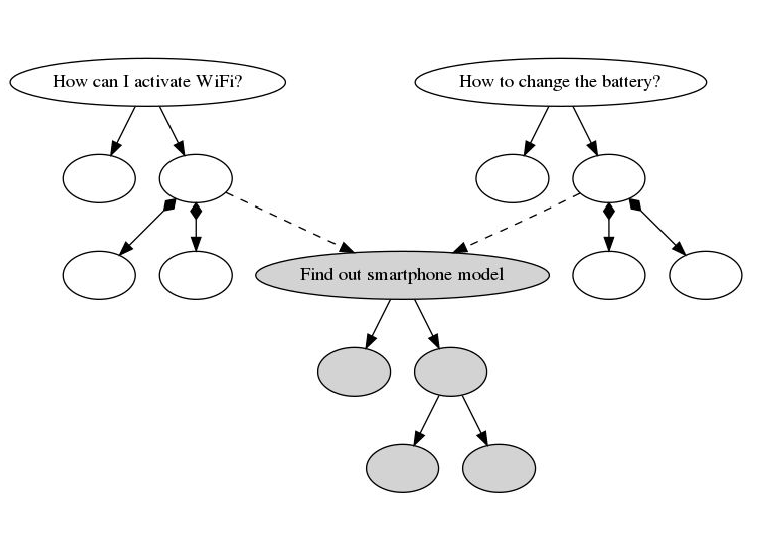
\includegraphics[width=0.9\textwidth]{img/Module_Reusability_2.PNG}
    \caption{Module usability within a chatbot}
    \label{fig:modReus2}
\end{figure} 
\\~\\
The same dialogue graph with a traditional dialogue tree is shown in Figure \ref{fig:modReus3} which has several restrictions and disadvantages. The module should be defined twice, more explicit relations needed to go back from one state to another and the dialogue trees are more complicated. Also the number of nodes and transitions will be higher as considered to Frankenbot's architecture resulting to higher processing as shown in the Table \ref{tab:tradVsFran}.
\begin{figure}[!h]
    \centering
    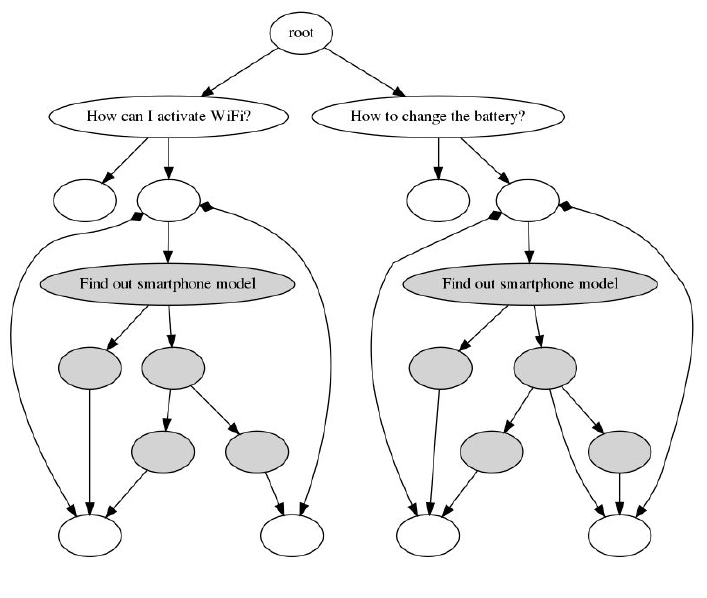
\includegraphics[width=0.9\textwidth]{img/Module_Reusability_3.PNG}
    \caption{Module usability within a chatbot}
    \label{fig:modReus3}
\end{figure}

\begin{table}[!h]
    \centering
   \begin{tabular}{ |c|c|c|c| } 
        \hline
         & No. of Nodes & No. of Transitions \\
        \hline
        \row{Traditional} & 21 & 26 \\ 
        \row{Frankenbot} & 15 & 14 \\ 
        \hline
    \end{tabular}
    \caption{Traditional vs. Frankenbot in terms of nodes and transitions}
    \label{tab:tradVsFran}
\end{table}

\item \textbf{Usability among different Chatbots:} Usability can be enhanced by using modular architecture. Multiple chatbots can share common modules. The module needs to be defined only once. Changes in the module will automatically be integrated in all chatbots. Figure \ref{fig:modReus} shows visuals for better understanding of it. 
\begin{figure}[!h]
    \centering
    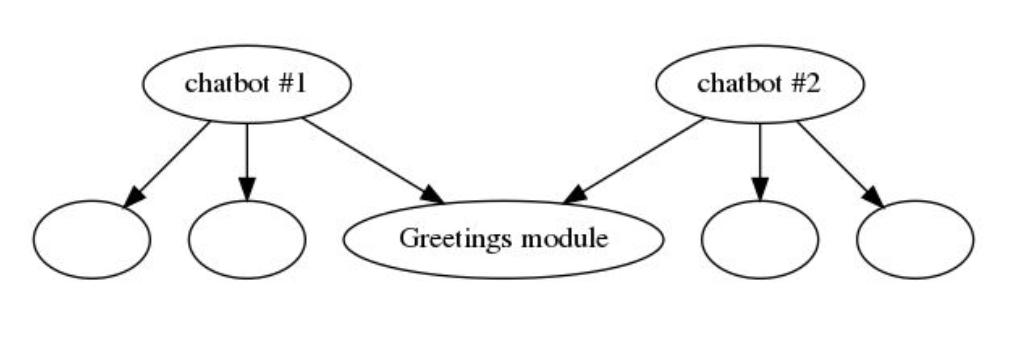
\includegraphics[width=0.9\textwidth]{img/Module_Reusability.PNG}
    \caption{Module usability between different chatbots}
    \label{fig:modReus}
\end{figure}       
\end{itemize} 

\paragraph*{Sense for Staying in the Topic}
The dialogue manager chooses the module with the highest activation function. But we can also add a term to stay in the topic: 
\begin{align*}
 Activation(module) = Z(utterance, state) + History(module)
\end{align*} 
Z is the activation function. History(module) is a term that gets bigger if the module has been active before. Therefore the module that was used before has a higher probability of being chosen which refers to the chatbot staying in the topic characteristic.

\section{Frankenbot: System Architecture}
Frankenbot’s system architecture has been sketched in Figure \ref{fig:sysArch}. It consists of a server and server-side web API. The user communicates using a browser and sends a request using web API to a server. Furthermore, the server contains the deployed Frankenbot's framework built using Python 3. Web server loads data for a chatbot from the JSON file for now but will be integrated with some database in the future. Whereas, a frontend for user's interaction has built simply using javascript, HTML, and CSS. Web API has been built using python library known as Flask \cite{flask}. 

\begin{figure}[!h]
    \centering
    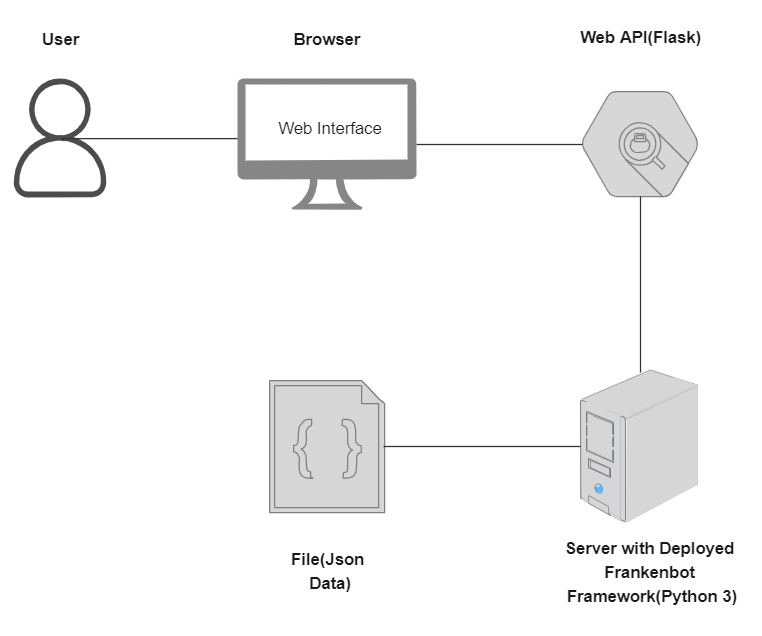
\includegraphics[width=0.9\textwidth]{img/System_Architecture_Updated.PNG}
    \caption{Frankenbot's System Architecture}
    \label{fig:sysArch}
\end{figure} 
\\~\\
As it is clear from Figure \ref{fig:sysArch} that the communication between the client and the server is possible only via web API composed of a simple get request. In addition to that when you dig deep into the framework, it is composed of several different components.

\subsection{RASA Framework for NLU \label{subsec:rasanlu}}
RASA is an open-source renowned conversational artificial intelligence framework for designing contextual virtual agents. It is a machine learning framework designed to communicate through automated text and voice-based techniques. \cite{rasa}
\\~\\
For making it work, the following steps must be taken into account:
\begin{enumerate}
    \item Provide training data \cite{rasatrainingdata}.
    \item Provide configuration file with pipelines for training \cite{rasapipeline}.
    \item Provide directory's path to save trained models.
    \item Generate rasa interpreter by loading it from the trained models' directory.
\end{enumerate}
For utilizing it in a Frankenbot, necessary steps have been mentioned below under the heading of Configurations.
% \ref{par:config} in Frankenbot's Framework.
 
\subsubsection*{Training for RASA NLU}
It has been used for natural language understanding in Frankenbot. It needs to get trained first to produce some useful results and for that purpose, one needs to provide it with the training data. It can be provided using different formats as mentioned on its website \cite{rasatrainingdata}. For Frankenbot, JSON format has been adopted but it can be changed without any issue based upon the developer preferences. This format consists of a top-level object called rasa\_nlu\_data, with the keys common\_examples, entity\_synonyms, and regex\_features. The most important one out of these all is common\_examples.

\begin{lstlisting}[language=json,firstnumber=1]
{
    "rasa_nlu_data": {
        "common_examples": [],
        "regex_features" : [],
        "lookup_tables"  : [],
        "entity_synonyms": []
    }
}
\end{lstlisting}
 Moreover, common\_examples are a list of objects with the keys text, intent, and entities. Whereas, entities can be an empty list or the objects list with the keys start, end, value, and entity.
 
 \begin{lstlisting}[language=json,firstnumber=1]
{
    "text": "...",
    "intent": "#...",
    "entities": [
            {
                "start": ...,
                "end": ...,
                "value": "...",
                "entity": "@..."
            },
            ...
    ]
}
\end{lstlisting}

\subsection{Frankenbot Framework}
This framework is composed of various components. Each of which is responsible for performing a specific task. It has been majorly divided into the following two divisions: (i) The web server(backend), which is responsible for the creation of the whole chatbot and producing desired responses for a user and (ii) A client(frontend) also known as a user interface to interact with a chatbot. Both of these are explicitly explained below.
\\~\\
The detailed diagram for Frankenbot's Framework Architecture has been portrayed in Figure \ref{fig:frankArch}. All the components have been discussed in detail.

\begin{figure}[!h]
    \centering
    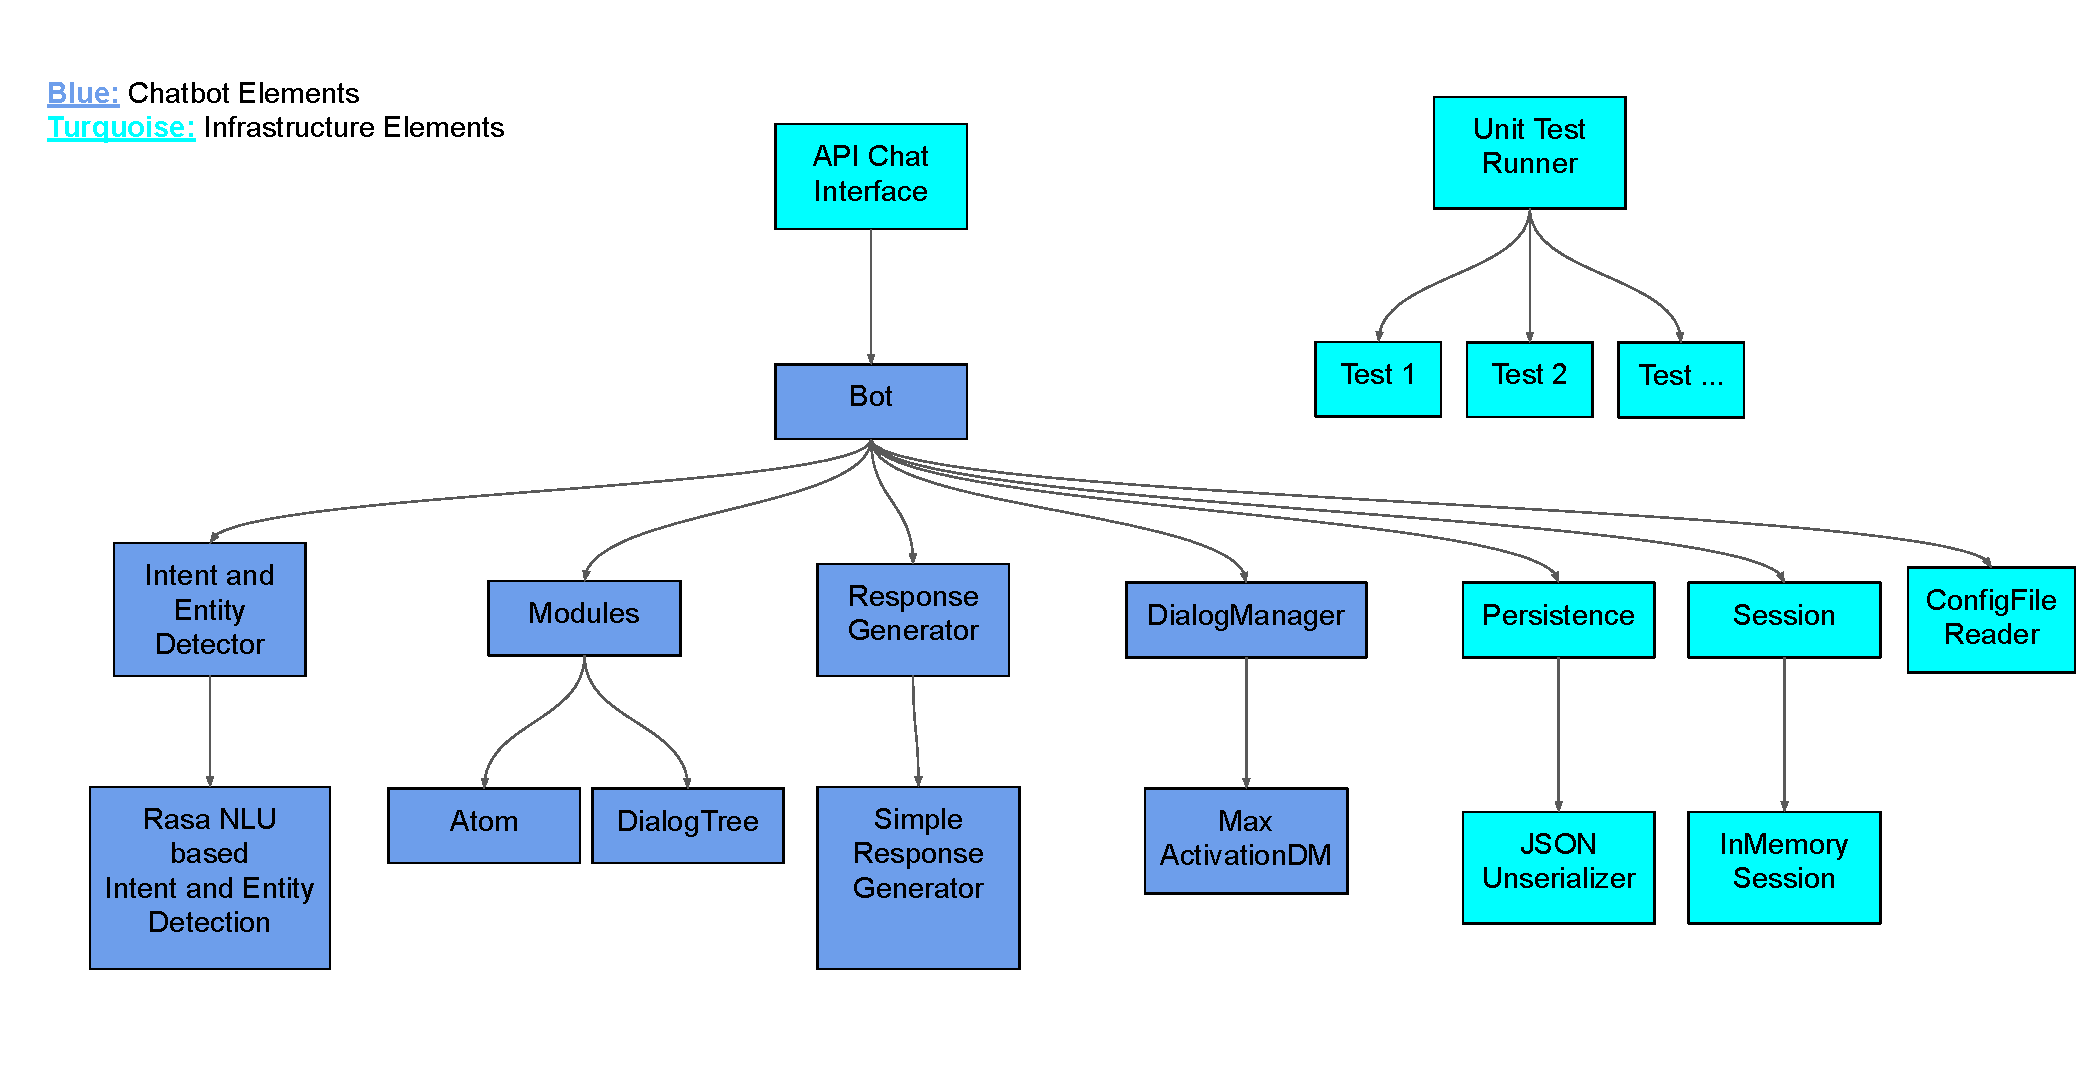
\includegraphics[width=0.9\textwidth]{img/Frankenbot_Architecture_Diagram_Updated.pdf}
    \caption{Frankenbot Framework Architecture Diagram}
    \label{fig:frankArch}
\end{figure} 

\subsubsection*{Client}
It is implemented using simple JavaScript, Html, and CSS. The template can be found under \cite{userinterface}. It is a simple user interface for a chat which allows a user to type a message and send it to the server by making simple get request utilizing the web API. 
\\~\\
Furthermore, it is also responsible for storing the user's session id to storage on a browser. For that purpose browser's "localStorage" \cite{localstorage} is used. If the user is connected to the first time to the server then it requests an empty session id and user utterance to the server. And as a response chatbot sends a welcome message and assigns an id to a user. Which is saved in the browsers local storage for every user. Whenever there comes a new request from this user to a server, the session id is being sent along with a user utterance to a server. In return, the server responds with a suitable response according to the user utterance which is being displayed next to the last user utterance. The response from the server is in the form of a JSON object which is being parsed to extract the chatbot's reply and displayed for a user. The important point to take into account is that the user id will be stored until the page is not reloaded or closed. If you want to restart your session and get away with all your previous chat, then you can simply refresh the web page and it will make a new instance of the chatbot. But for the future, a server will have the record of all dialogues that happened in a past stored in a database. 
\\~\\
For better understanding graphical representation for an interface is shown in Figure \ref{fig: userInter}.

\begin{figure}[!h]
    \centering
    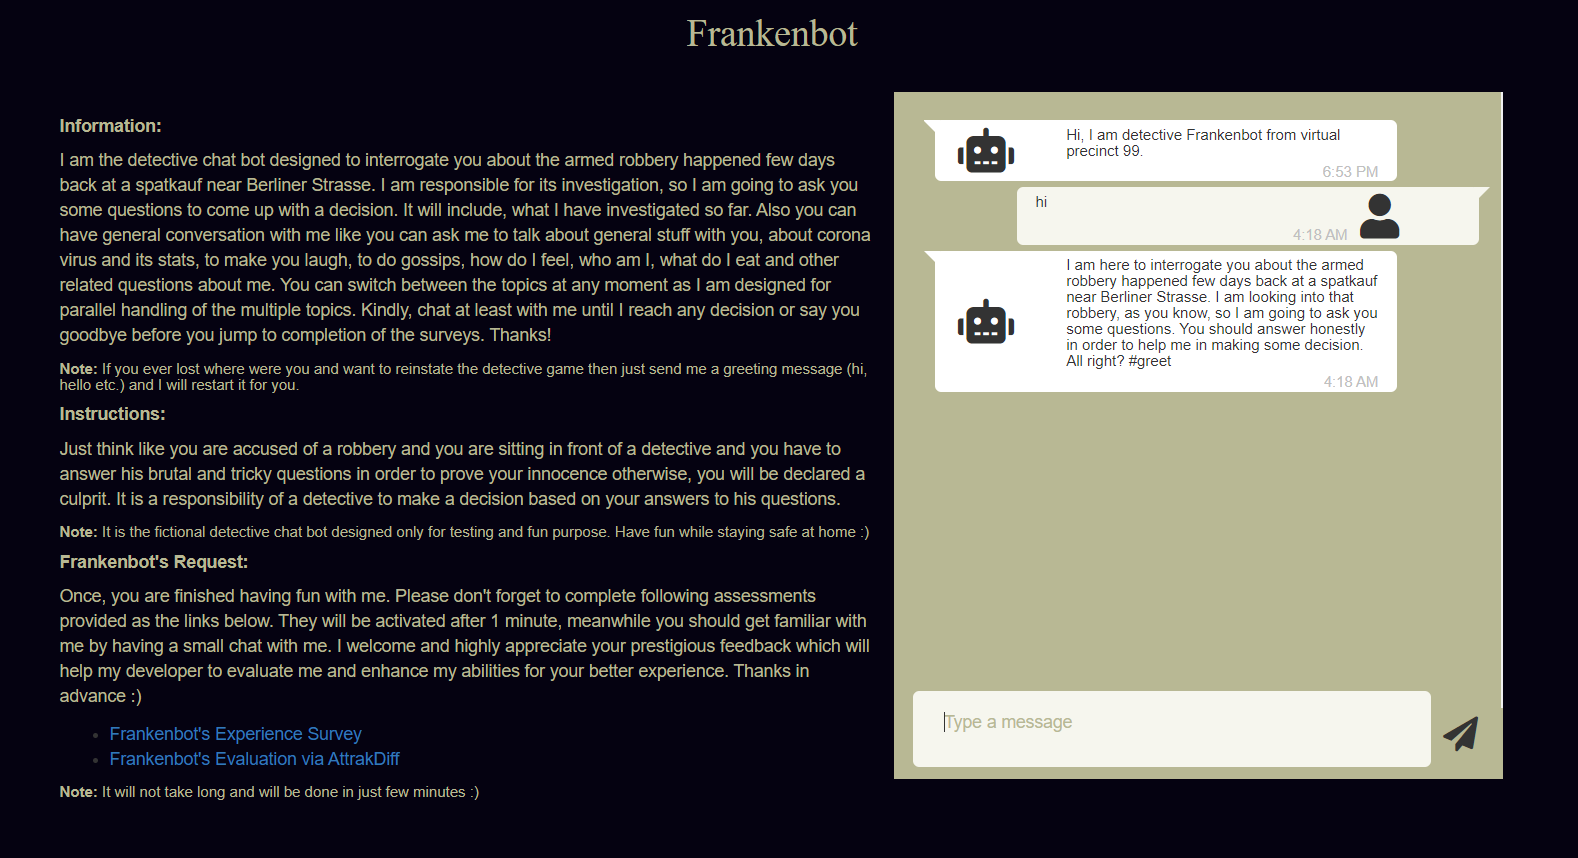
\includegraphics[width=0.9\textwidth]{img/User_Interface.PNG}
    \caption{Frankenbot's User Interface(Client)}
    \label{fig:userInter}
\end{figure}
\\~\\
As demonstrated, the left side of the screen contains important information and instructions for a new user. Whilst, on its right, there exists a chatbox showing the first most message as a welcome message for the newly arrived user. After that the chat between the user and a bot initiated. The user can type a message in the bottom-most text box and press sends button or enter button from keyboard. The user's message will be displayed on the left side of the screen while the response will be shown on the right side of the screen's display and vice-versa according to your viewpoint.

\subsubsection*{Web Server}
The web server itself is a composite of multiple classes performing specific tasks and connected to a client using web API. It is written in Python version 3. Abstractly, it is responsible for performing all tasks required to make a chatbot functioning. Firstly it receives user utterance as a parameter and initializes a chatbot from data provided as a source file of the JSON format. After initializing a chatbot, it undergoes various actions for a user utterance to generate a response.

\paragraph*{Infrastructure Elements}

\subparagraph*{Web API}
It is implemented using the python library known as Flask. It is responsible for making a connection between the user and a server. It makes a user communicate with a server. Whenever there comes a new request from the client, firstly it passes from the function implemented for its handling.
\\~\\
Important tasks performed by the web API are:
\begin{enumerate}
    \item Receiving the user utterance and session id as a parameter from the get request made by the client.
    \item Checking whether the session id already exists or its a new user. If it happens to be a new user then there will be the empty user utterance and user session-id received as a parameter from the client's get request. It will initialize a chatbot using the data provided in the JSON file (discussed in detail below). Afterward, it assigns a new user session id and sends it along with a welcome message as a response to a client.
    \item If a session already exists, then it checks for the current dialogue state for an active user. And instead of initializing a new chatbot, the chatbot with the last stored state is being traversed with a new user utterance to get an appropriate response. And before responding to the client the current state gets updated again and stored for the current user.
     \item The response is being sent as a JSON object.
\end{enumerate} 

\subparagraph*{Persistence}
Persistence includes the Json Unseralizer. It takes the JSON file as an input and parses it for generating an initial chatbot.
\\~\\
The JSON file contains data as a JSON dictionary object which includes the name of a bot, welcome message, fallback message in case of no response, and a dialogue manager. Inside a dialogue manager, there exists a list of modules consisting of several modules having unique module ids. Additionally, each module contains a dialogue tree having a list of tree nodes. Whereas, each tree node includes a unique node id, information about its parent node, name of intent to which it belongs, and respective response generator. Furthermore, a response generator includes a mode for the responses that can be sequential or random and a list of responses. And all of the above-mentioned elements are uniquely identified using a key "type". For better understanding, just have a look at a JSON sample shown below:
\\~\\
% caption=A first example
\begin{lstlisting}[language=json, firstnumber=1, label={lst:botJson}]
{
  "type": "bot",
  "name": "...",
  "welcome_message": "Hi, ...",
  "fallback_message": "any desired message for bot's failure.",
  "dialog_manager": {
    "type": "max_activation_dialog_manager",
    "modules": [
        {
        "type": "dialog_tree",
        "module_id": "module1 or any id",
        "dialog_tree": [
          {
            "type": "tree_node",
            "node_id": any integer e.g 1,
            "parent_node": null for making root or any node id  to assign it a parent,
            "intent_name": "#...",
            "response_generator": {
              "type": "simple_response_generator",
              "mode": "sequential or random",
              "responses": [
                ...,
                ...
              ]
            }
          },
          ... ,
        ]
      },
      ... ,
    ]
  }
}
\end{lstlisting}
\\~\\
Theoretically, a bot is composed of a dialogue manager that contains information about all the modules representing the entire dialogue structure. Moreover, a module includes a dialogue tree that has been developed to design a dialogue. Each dialogue tree is made up of the relational tree nodes. And each tree node holds all the technical information about the intent and other required fields for a dialogue to produce the respected response.
\\~\\
Now coming towards practical implementation, a bot is generated recursively based on unique type key. The JSON data has been iterated and checks for the type of each element recurrently. And by taking that type of element into account, it returns the object for different respective classes. Let suppose the JSON object contains types in the following sequence:
\begin{enumerate}
    \item bot; recall the same function with a JSON for a dialogue manager returns a class Bot's object afterward.
    \item max-activation-dialogue-manager; recall the same function with a JSON for each module in a list of modules and returns a class MaxActivationDialogueTreeManager's object afterward.
    \item dialogue-tree; recall the same function with a JSON for a dialogue tree and returns a tree consisting of tree nodes afterward.
     \item tree-node; recall the same function with a JSON for each element of a list dialogue tree and returns a class Atom's object afterward.
     \item simple-response-generator; recall the same function with a JSON for a response generator and returns a class SimpleResponseGenerator's object afterward.
\end{enumerate} 
Now the function initiates and finds the very first type "bot" in a JSON data shown above. And then the recursive call to the same function is sent with "dialogue\_manager" JSON object. Likewise, sequential recursive calls happen for types "modules", dialog\_tree" and "response\_generator" with their specific JSON objects. Once it reaches the last key type "simple\_response\_generator" then it starts returning the corresponding class object related to each type as listed before. So, the function starts executing from the first step mentioned above but starts returning recursively from the last step. It means, the class SimpleResponseGenerator's object is passed as a parameter to the constructor of the upper-level class object i.e. class Atom in this case. The same goes for all other classes. In this way, class SimpleResponseGenerator's object gets appended to the class Atom's object, and so on. Finally, the class Bot object should contain the class MaxActivationDialogueManager's object as an attribute and that is how the chatbot will be generated recursively.
\\~\\
Also, there is a convention used to represent the intents, entities, and context variables. It has been taken from the state of the art chatbot IBM Watson as the intent is denoted by prefix "\#", an entity is denoted by "@" and "\$" symbol is used to denote a context variable. Same convention has been used in Frankenbot as shown in the Table \ref{tab:repIntEntCont}.

\begin{table}[!h]
    \centering
   \begin{tabular}{ |c|c|c|c| } 
        \hline
         & Key & Value \\
        \hline
        \row{Intent} & {\#intent\_name} & {intent\_value} \\ 
        \row{Entity} & {@entity\_name} & {entity\_value} \\
        \row{Context Var.} & {\$context\_var\_name} & {context\_var\_value} \\
        \hline
    \end{tabular}
    \caption{Representation for an Intent, Entity and Context Variable}
    \label{tab:repIntEntCont}
\end{table}


\subparagraph*{Session}
It is responsible for session handling. It is subjected to establish "InMemorySession" which is meant to store session id in a list of session variables, context variables, and sequential response counter for each user. For each user, there exists a different chatbot's state. 
\\~\\
Whenever there comes a new user, the new dictionary object has been declared to store session id for a user along with its bot's state, active module id, and active node for each module. In addition to that, the last user utterance also gets stored for generating the last bot's message to the user if the chat window has been refreshed or reopened in a new tab of browser by a user(can be implemented in future). And then that dictionary object gets appended to a list of session variables. Which means there exists a separate object for each user in a list. It gets updated on every request from the client.
\\~\\
Another element present to save the context of dialogue for each user is known as context variables. They are independent of modules and get detected by NLU within a user utterance based upon the entities provided within the training data.  It is a dictionary having a user session id as a key, and each key represents a key-value pair for entities that appeared in a dialogue. Each entity name appeared in dialogue has been saved as \$EntitytName as a key and a value of the entity as its value. Its value gets updated every time if the same entity has been triggered or a new entity has been discovered in a dialogue for the same user. These context variables are used to understand the context of dialogue and update the entity value in a response if it is intended.
\\~\\
Another important attribute available is the response sequential counter. Its main task is to keep track of all intent's response counter for each user if its mode has been set to sequential. It means if an intent contains multiple responses and the bot has to produce a response for it based on the user utterance then each time the next response should be produced for a user. It is intended to give a more realistic impression to a user and human-like interaction behavior to a dialogue.

\subparagraph*{Configurations \label{par:config}}
To make chatbot work it is really important to provide it with proper configurations. Frankenbot needs three following directories to function:
\begin{enumerate}
    \item bot directory; It should be provided with the bot's directory name as a command-line parameter while running the project. For example, the running command in my case is "python app.py detective". In this command "detective" is the name of a directory which should contain JSON file for initializing a bot. And it should be named "frankenbot.json" (see Appendix \ref{appen:frankJson} to have a look at actual JSON data used for the structuring of the Frankenbot). 
    \item Furthermore, the bot directory must contain training data directory named as "rasa". Firstly, this sub-directory must contain a configuration file named as "config\_spacy.yaml" defining pipelines required for Rasa NLU Training\cite{rasapipeline} (see Appendix \ref{appen:rasaConf} to have a look on actual pipelines used). Secondly, JSON files must be available with training data for each module in "frankenbot.json". And the names for those training files should be the same as module id assigned to a module for which it contains training data. For example, "frankenbot.json" contains two modules, and ids assigned to them are detective\_tree and general\_tree. So, the training files should be named "detective\_tree.json" and "general\_tree.json" (see Appendix \ref{appen:trainDF} to have a look at actual JSON training data used for both training of modules in the Frankenbot).
    \item Lastly, the model directory is required to store the rasa models produced after the model gets trained for each module. It can be any directory but one has to provide an appropriate path to it.
\end{enumerate} 

\paragraph*{Chatbot Elements}

\subparagraph*{Bot} Once the initial bot is generated, it is the very first element that has been instantiated. Originally it contains the complete definition for a chatbot. Which includes attributes such as chatbot's name, welcome message, fallback message, and most importantly dialogue tree manager(discussed below in next heading).
\\~\\
Whenever a request from a client has been made it firstly gets processed by this component. As it receives the user utterance, active tree nodes for each module for a particular user and session information as the parameters. 
\\~\\
Complete flow can be observed in Figure \ref{fig:flowBot}. The parameters are further passed to the dialogue tree manager to find a module with the highest intent's activation value, detected intent, intent's activation value, detected entities, entities activation values, active tree node, active module id, and JSON output object. This JSON object has been returned to a client containing all important information and respective response.
\\~\\
Before returning the response as a JSON object, it is also responsible for performing some major tasks. Firstly, it checks for detected entities received after the processing of its dialogue tree manager. If there exists any detected entity then entity(s) in the context variables for a particular user gets added or updated depending upon the current state of a bot.
\\~\\
In addition to that, it also checks for the detected intent's activation value for a user utterance. As Rasa's NLU has been used to detect the intent and there are the chances of getting a false result with very low activation value. So it checks for it and responds only if its value lies above some threshold. The range of activation value lies between 0 and 1. If the value is below the threshold then it checks for the last active node for a user whether it exists or not. If it doesn't exist then, it means the user started a chat with some meaningless utterance as an input for a bot. So, the chatbot should respond using node with intent anything\_else if it exists in a module with the highest activation obtained from RASA's NLU result. Secondly, if there exists some chatbot's active state for a user, then it checks for the last active module for a user and also checks for a node with an intent name anything\_else in its children. If it is available then the response has been generated using it. Otherwise, it simply responds with a fallback message.
\\~\\
Alternatively, if it is above the threshold then the highest module received from its dialogue tree manager has been used to generate an appropriate response(explained ahead).

\begin{figure}[!h]
    \centering
    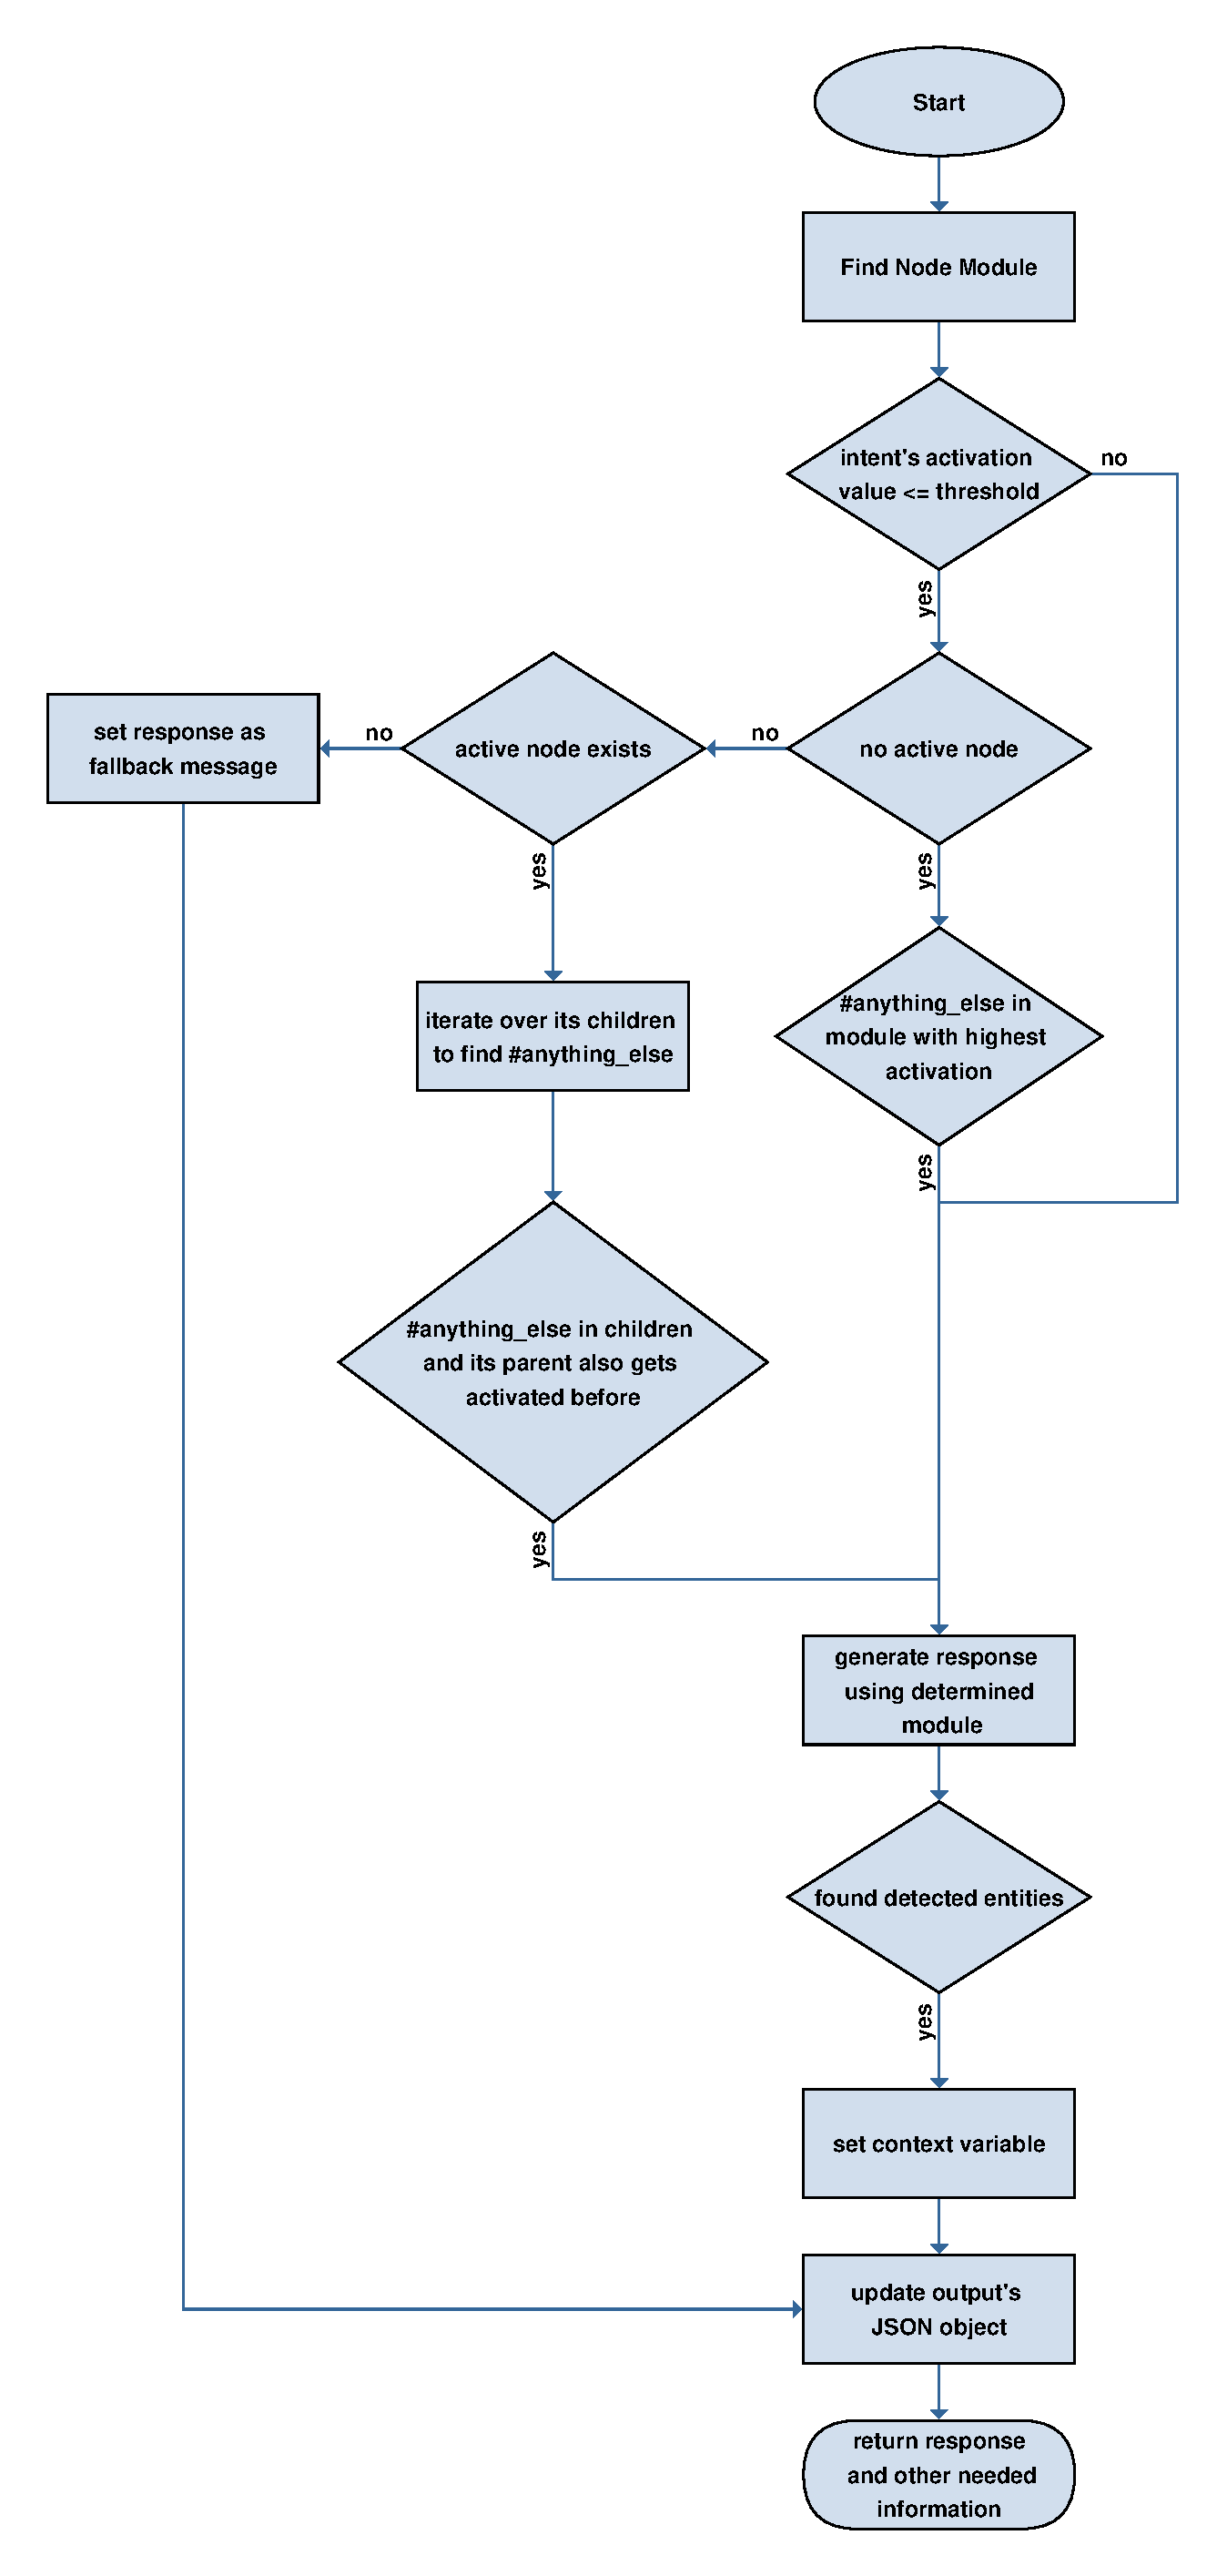
\includegraphics[width=0.6\textwidth]{img/bot.pdf}
    \caption{Flow chart for the bot's say function}
    \label{fig:flowBot}
\end{figure}

\subparagraph*{Dialogue Manager} Dialogue manager is an abstract class whereas the max activation dialogue tree manager is an inherited class that should implement the abstract functions of a dialogue manager. Max activation dialogue manager originally contains the dialogue tree, once the chatbot has been initialized. Now the question arises what is the dialogue tree composed of? So, the dialogue tree gets generated while chatbot is loaded from the JSON file. And it is composed of the list of tree nodes, unique module id, data for RASA's NLU training and interpreter loaded from model directory once the training has been finished. Whereas, each tree node contains unique node id, information about its parent node,  intent, activation flag which gets set if it is responsible for generating a response, and a module object which itself consists of the intent detector and response generator. The dialogue tree has been generated using the python library "any tree" \cite{anytree}.
\\~\\
A detailed visual chart for a dialogue manager is portrayed below in Figure \ref{fig:flowDialogueMan}. It is responsible for finding a module with the highest activation based upon the detected intent's activation value for the user utterance. So for this purpose, each tree must be traversed for each of its nodes. As each node contains a module object which is further utilized for this purpose. Module's activation function is being called bypassing user utterance, RASA interpreter for the current module, module id for a recent module, and session data as parameters. And it returns activation value for each intent along with its name, recognized entities along with their activation values and the JSON object for output. As activation function for all nodes in each tree has been called and meanwhile dialogue manager keeps on checking for the activation value received for each node's module. And keeps on updating it whenever the last received value is greater than the previously stored value. In this way, the module with the highest activation is detected.
\\~\\
Responsibility of a dialogue manager not only ends here but it is also responsible to make the chatbot follow the modular architecture which is the main goal behind the designing of the Frankenbot. As explained above about the modular architecture that how should it work, let's discuss it here in a technical perspective. Whenever, the recently received activation value is greater than the last stored activation value and the identified intent is same as the current node's intent name then there comes following scenarios, if the recently traversed node is a root node or not: 
\begin{enumerate}
    \item If it is a root node then its activation flag should be set so that for the next time its children can be accessed for response generation. Also, all the required information must be stored and returned to the previously discussed bot component. Which is responsible for returning the response to the client via web API and the active state for the current user must get updated beforehand. 
    \item Secondly, if the recently processed node is not a root node then what should be its behavior? It is a bit complex strategy to follow. Firstly, it should check if its parent's activation flag is set or not. If it is set then it should proceed further otherwise it should not. Let's suppose that it is set and it steps ahead and finds multiple nodes with the same intent in its children nodes then it will not respond correctly. As it is the main idea behind the modular architecture that modules can be reused but different modules with the same intents do not need to have the same responses. Responses can differ at different levels in a tree whilst having the same intent. So for removing this problem, an active state for each module has been stored separately. This means if there exist two modules for a chatbot then there should be two separate active states, one for each module, available for a user. So by using these active states, it can match the last active node's id with the current node's parent id and if it is true then it is good to go. Also what if the user starts to enter the same user utterance again and again. It will again cause a problem as it will be searching for intent in the last active node's children but it will not be able to find it. So to overcome this issue, the manager matches the current node's id with the last active node's id and again if this condition has been satisfied then it should respond correctly. 
    \item Lastly, irrespective of the above conditions whether any of them is satisfied or not. It should return to a bot component which is meant to handle all scenarios and responsible to produce an appropriate response if there exists any highest detected module. Otherwise, it uses anything\_else node or fallback message to respond depending upon the state and design of the bot.
\end{enumerate} 
\\~\\
In the end, it also checks for identified entities and their activation values and stores and updates them accordingly. And all the essential information is returned to a bot component. Which is responsible for returning the response to the client via web API and the active state for the current user should be updated beforehand.

\begin{figure}[!h]
    \centering
    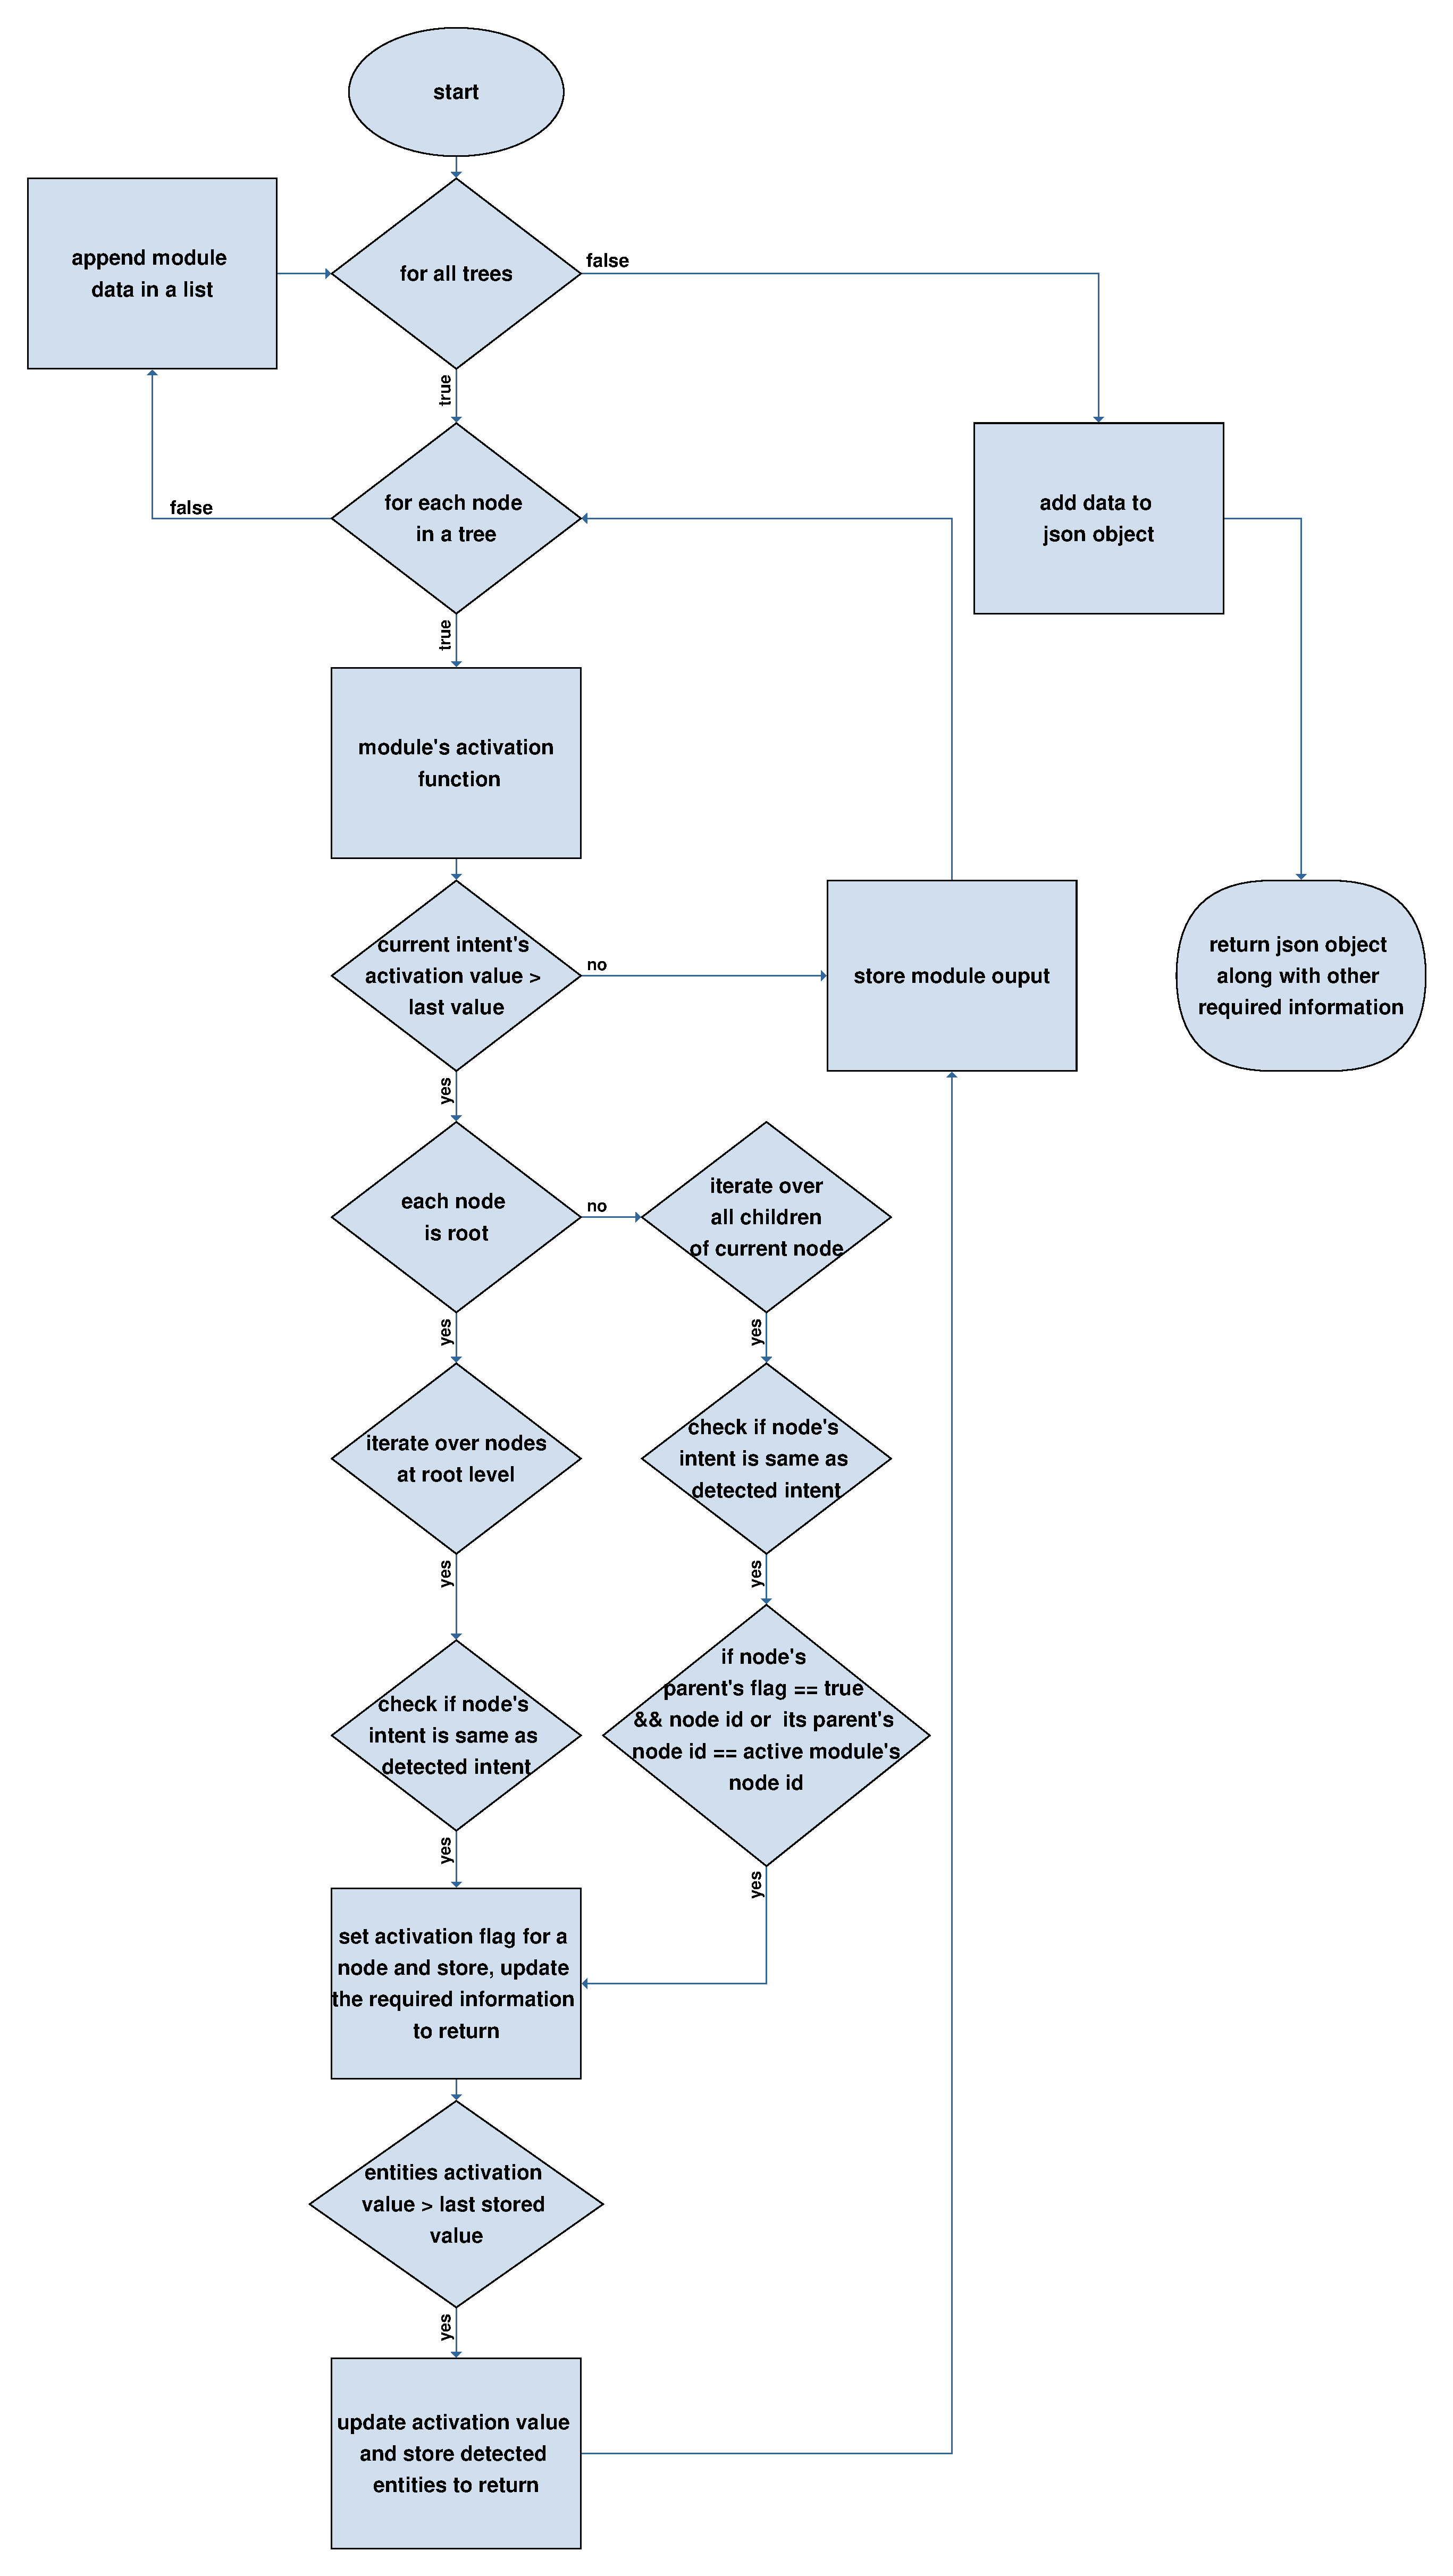
\includegraphics[width=0.7\textwidth]{img/Dialogue_manager.pdf}
    \caption{Flow chart for the dialogue manager's find node module function}
    \label{fig:flowDialogueMan}
\end{figure}

\subparagraph*{Modules} Modules class is responsible for generating activation value for each intent which is passed to the dialogue manager for further processing as described above. In addition to that, it is also pledged for generating responses and JSON objects for API output. So these three functionalities should be implemented in a class inherited from abstract modules class. So, class Atom is inherited from it and provides all functional definitions for abstract class. 
\\~\\
There are two attributes needed for the atom class. One is natural language understanding(NLU) which is an object for rasa intent and entity detector and second is a simple response generator's object, Both of these components have been described next under their respective headings. 
\\~\\
Starting with an activation function is graphically represented in Figure \ref{fig:flowModule}. It initiates from a max activation dialogue manager's function to find a node's module with the highest activation value, all trees are traversed for each corresponding node. Each node contains a particular module object with its NLU and response generator. Using that module, activation function has been called provided user utterance, rasa interpreter, recent module id for a tree, and session information as parameters to it. And what it does with these parameters received is, it passes them further to make a call for natural language understanding to detect intents and entities. And the encountered intents and entities are then further passed for creating JSON object to return to the client as an API output. 

\begin{figure}[!h]
    \centering
    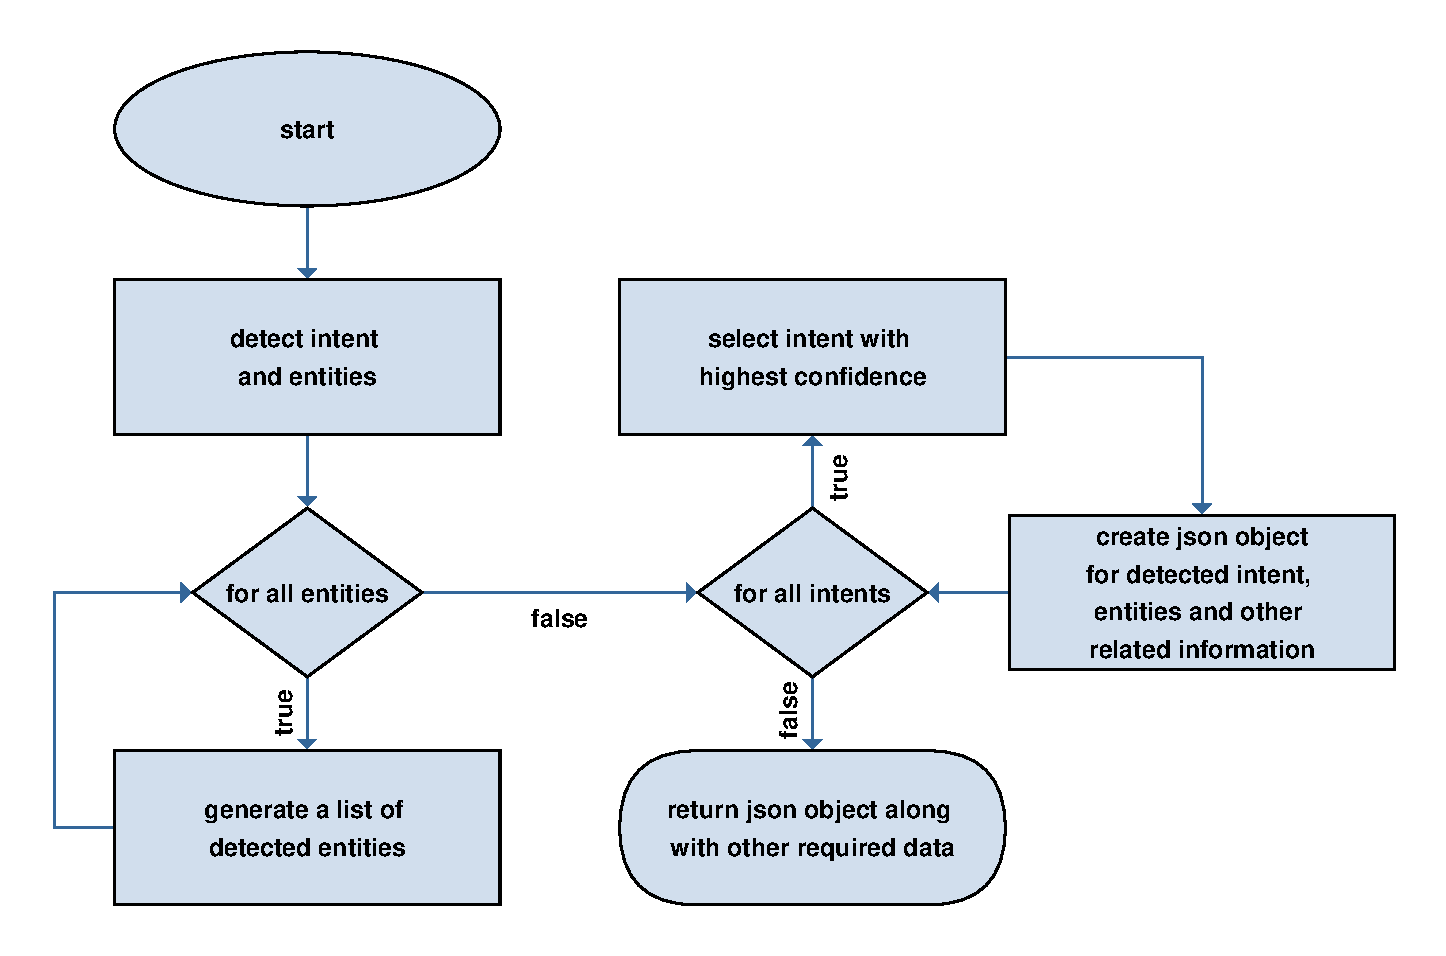
\includegraphics[width=0.9\textwidth]{img/module.pdf}
    \caption{Flow chart for the module's activation function}
    \label{fig:flowModule}
\end{figure}
\\~\\
Moreover, it also has been used to generate a response with the help of the response generator for an encountered module with the highest activation based upon the identified intent and entities for a particular user.

\subparagraph*{Intent and Entity Detection}
It is one of the basic and necessary components for all chatbots. The same applies to Frankenbot. An intent and entity detector is responsible for the identification of intent and entities for a user utterance. So this feature must be handled within a successor class for it. So rasa intent entity detector is implementing this functionality for an abstract parent class.
\\~\\
Each tree node consists of an atom and each atom consists of the intent and entity detector with the intent and entities information stored for each node. Visuals for it have been displayed in Figure \ref{fig:flowIntandEnt} exhibiting a comprehended process. It is responsible to detect the intent and all the entities for the user utterance by utilizing the parametric RASA interpreter passed to it from the atomic activation function.
\\~\\
Coming towards internal processing, the user utterance is passed to the trained rasa interpreter to detect the intent and entities and matched with the current node's intent. If they have been appeared to be identical then the intent name is stored as a key in a dictionary object and a confidence value received from the result of the RASA interpreter represents its value. Also, the entities are stored as a list of dictionary objects and each object contains key-value pairs for entity name and confidence value, starting and ending index in an utterance. These detected intent and entities are returned from this function to its origin for further handling.

\begin{figure}[!h]
    \centering
    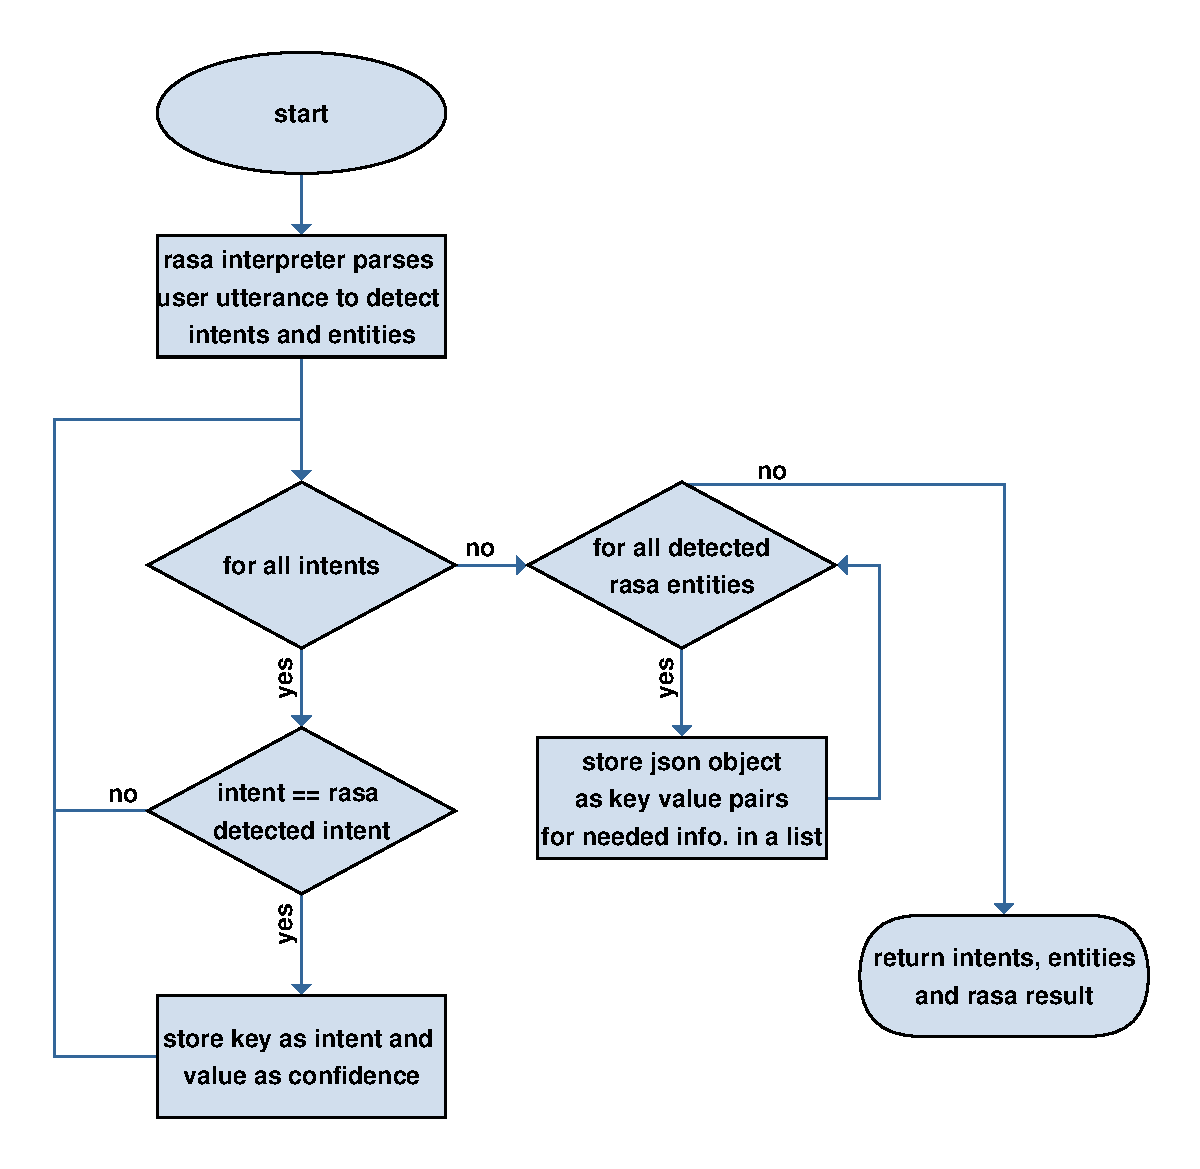
\includegraphics[width=0.9\textwidth]{img/Intent_entity_detector.pdf}
    \caption{Flow chart for the Rasa Intent and Entity Detector}
    \label{fig:flowIntandEnt}
\end{figure}

\subparagraph*{Response Generation}
As the name itself is self-explanatory that what task should it perform. The response generator is liable for producing a response by taking an identified intent into the account. Additionally, it is also responsible for appending chatbot response to the final JSON object designed to be returned as an API output. 
\\~\\
The precedent classes must take in to account both of the functionalities that parent abstract class is responsible for. A simple response generator does it all for Frankenbot. As it needs mode for a response that can be sequential or random and a list of responses for a captured intent for response selection.
\\~\\
Once the pre-processing has been completed, means all the steps have been finished and the dialogue manager has returned the atomic module with the highest activation value and a chatbot needs to generate a response. Now, a bot uses that observed module to send a request to this component by providing it with recognized intents and entities along with session information as an input. So that it can go ahead and perform the task that it is responsible for. 
\\~\\
Its graphical representation is shown in Figure \ref{fig:flowRespGen} below. Firstly, it checks for the intent's sequential response counter for a specific user and updates it accordingly for next time usage. Secondly, after the selection of a response, it checks within a response for entities and context variables. If there is any detected entity for a user utterance and a response needs to be exchanged with its value then it should be handled here. Also, if there is any context variable stored previously for a user and bot's reply needs to get modified with its value then it should also be done here. After all, processing has been accomplished, it should create a JSON object with a chatbot response for web API output and send it back to a bot component for performing next required executions. 

\begin{figure}[H]
    \centering
    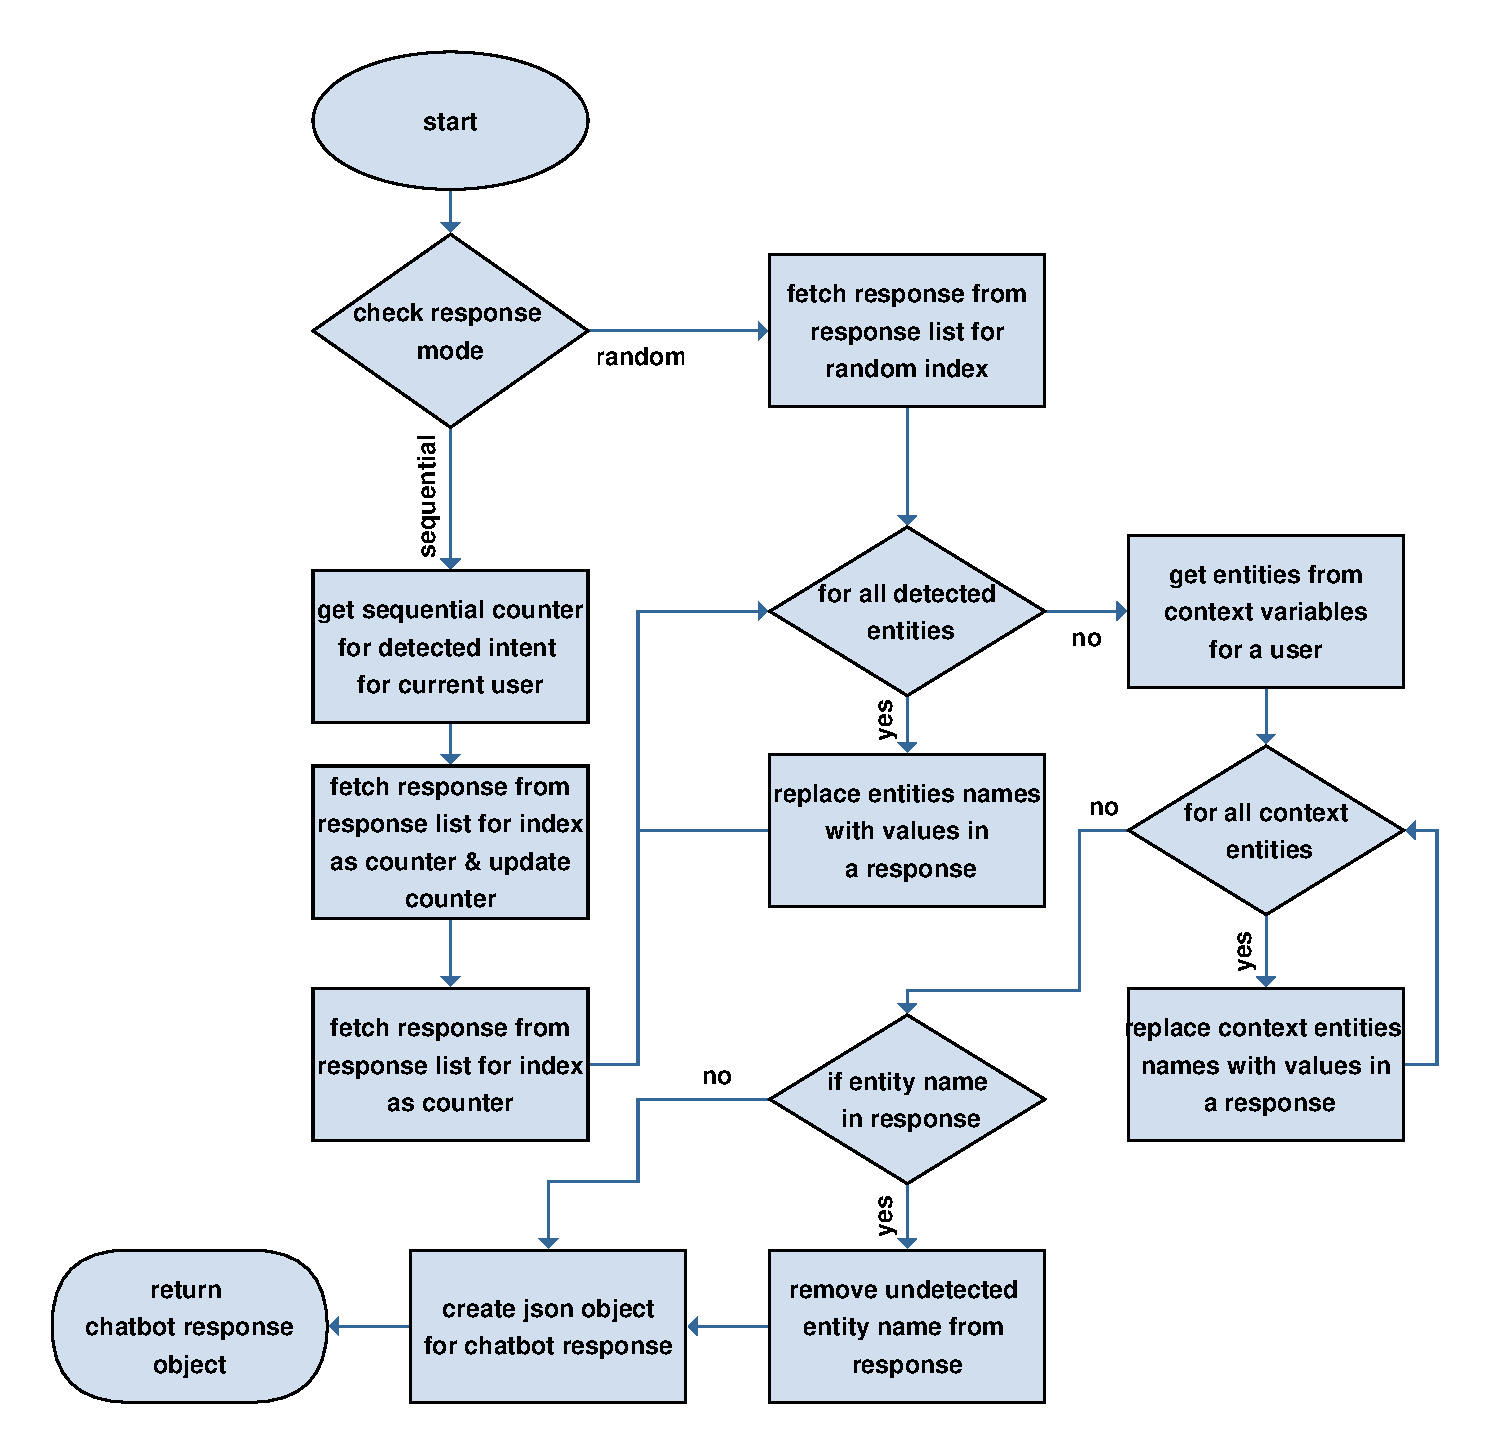
\includegraphics[width=0.9\textwidth]{img/Response_generator.pdf}
    \caption{Flow chart to generate response }
    \label{fig:flowRespGen}
\end{figure}

\subparagraph*{JSON API Output}
After all components are done with their part, bot returns a JSON object to web API which passes it further to a client which is parsed at the client side for displaying needed information for a user. Let's start with an observation of JSON object demonstrated below:

\begin{lstlisting}[language=json, firstnumber=1]
{
    "user_utterance": {
        "text": "..."
    }, 
     "chatbot_utterance": {
        "type": "simple_response", 
        "response": "..."
    },
    "active_module": {
        "id": "...", 
        "type": "dialog_tree_module", 
        "activation_value": ..., 
        "module_output": {
            "recognized_intent": "...", 
            "recognized_entities": []
        }
    }, 
    "modules_output": [
        {
         "id": "...",
         "type": "dialog_tree_module",
         "activation_value": ... ,
         "module_output": {
            "recognized_intent": "...",
            "recognized_entities": [],
            "intent_ranking": [
               {
                  "name": "...",
                  "confidence": ...
               },
               ... ,
            ]
         }
      },
      ... ,
    ]
}
\end{lstlisting}
The JSON object contains user\_utterance which holds a key text for the user's message as a value. Secondly, chatbot\_utterance's response is a final reply by a chatbot. An active\_module reflects an id of the recognized module, activation\_value in terms of rasa's confidence value for an identified intent. Whereas, its child module\_output depicts an encountered intent and detected entities. Finally, modules\_output involves the dictionary object for all modules in a chatbot through which user utterance has been processed to generate a response after intent detection. So, id shows an id of a module, activation\_value is same just like as mentioned before for active\_module. Furthermore, module\_output is also similar to active\_module's module\_output but with an additional key for intent\_ranking. It is comprised of all the names for the intents and their respective confidence values obtained from rasa's trained natural language interpreter.

\subparagraph*{Logging}
It is something that has been used commonly nowadays to track the events occurring in any software or a system. 
\\~\\
For the framework, it has been implemented using python's library called "logging" \cite{logging}. Before returning the JSON object via web API to the client, this object with all the essential information from start i.e. received user utterance, till end i.e. generated suitable response, has been logged to a log file to keep track of the complete dialogue. Also, the log file contains the information for RASA's NLU training process and what intents and entities have been found in training data. Additionally, it also helps in tracking the error or reason of the chatbot failure, if any such event occurs.  



    \chapter{Experiments and Evaluations\label{cha:chapter4}}

To evaluate the Frankenbot's modular architecture on the basis of the user experience, the surveys has been conducted. 
\\~\\
For evaluation of this research, a link provided in Appendix \ref{appen:deplFrank} to the deployed chatbot has been shared with participants using different social platforms along with an introductory text about the purpose of the study. Random users were selected irrespective of their profession, study background and any race or gender discrimination. But the age limit constraint was set to be above 18. As participants were considered to be accused of a robbery and have to chat with a detective bot and answer his questions which can be a bit strict and straight forward for youngsters below 18. So the participant participated with the minimum age was 22. On contrary, the one with the maximum age was 34. And the average age calculated as 25.65 with the standard deviation of 2.37. Visuals have been shown in the Figure \ref{fig:ageGraph}.

\begin{figure}[!h]
    \centering
    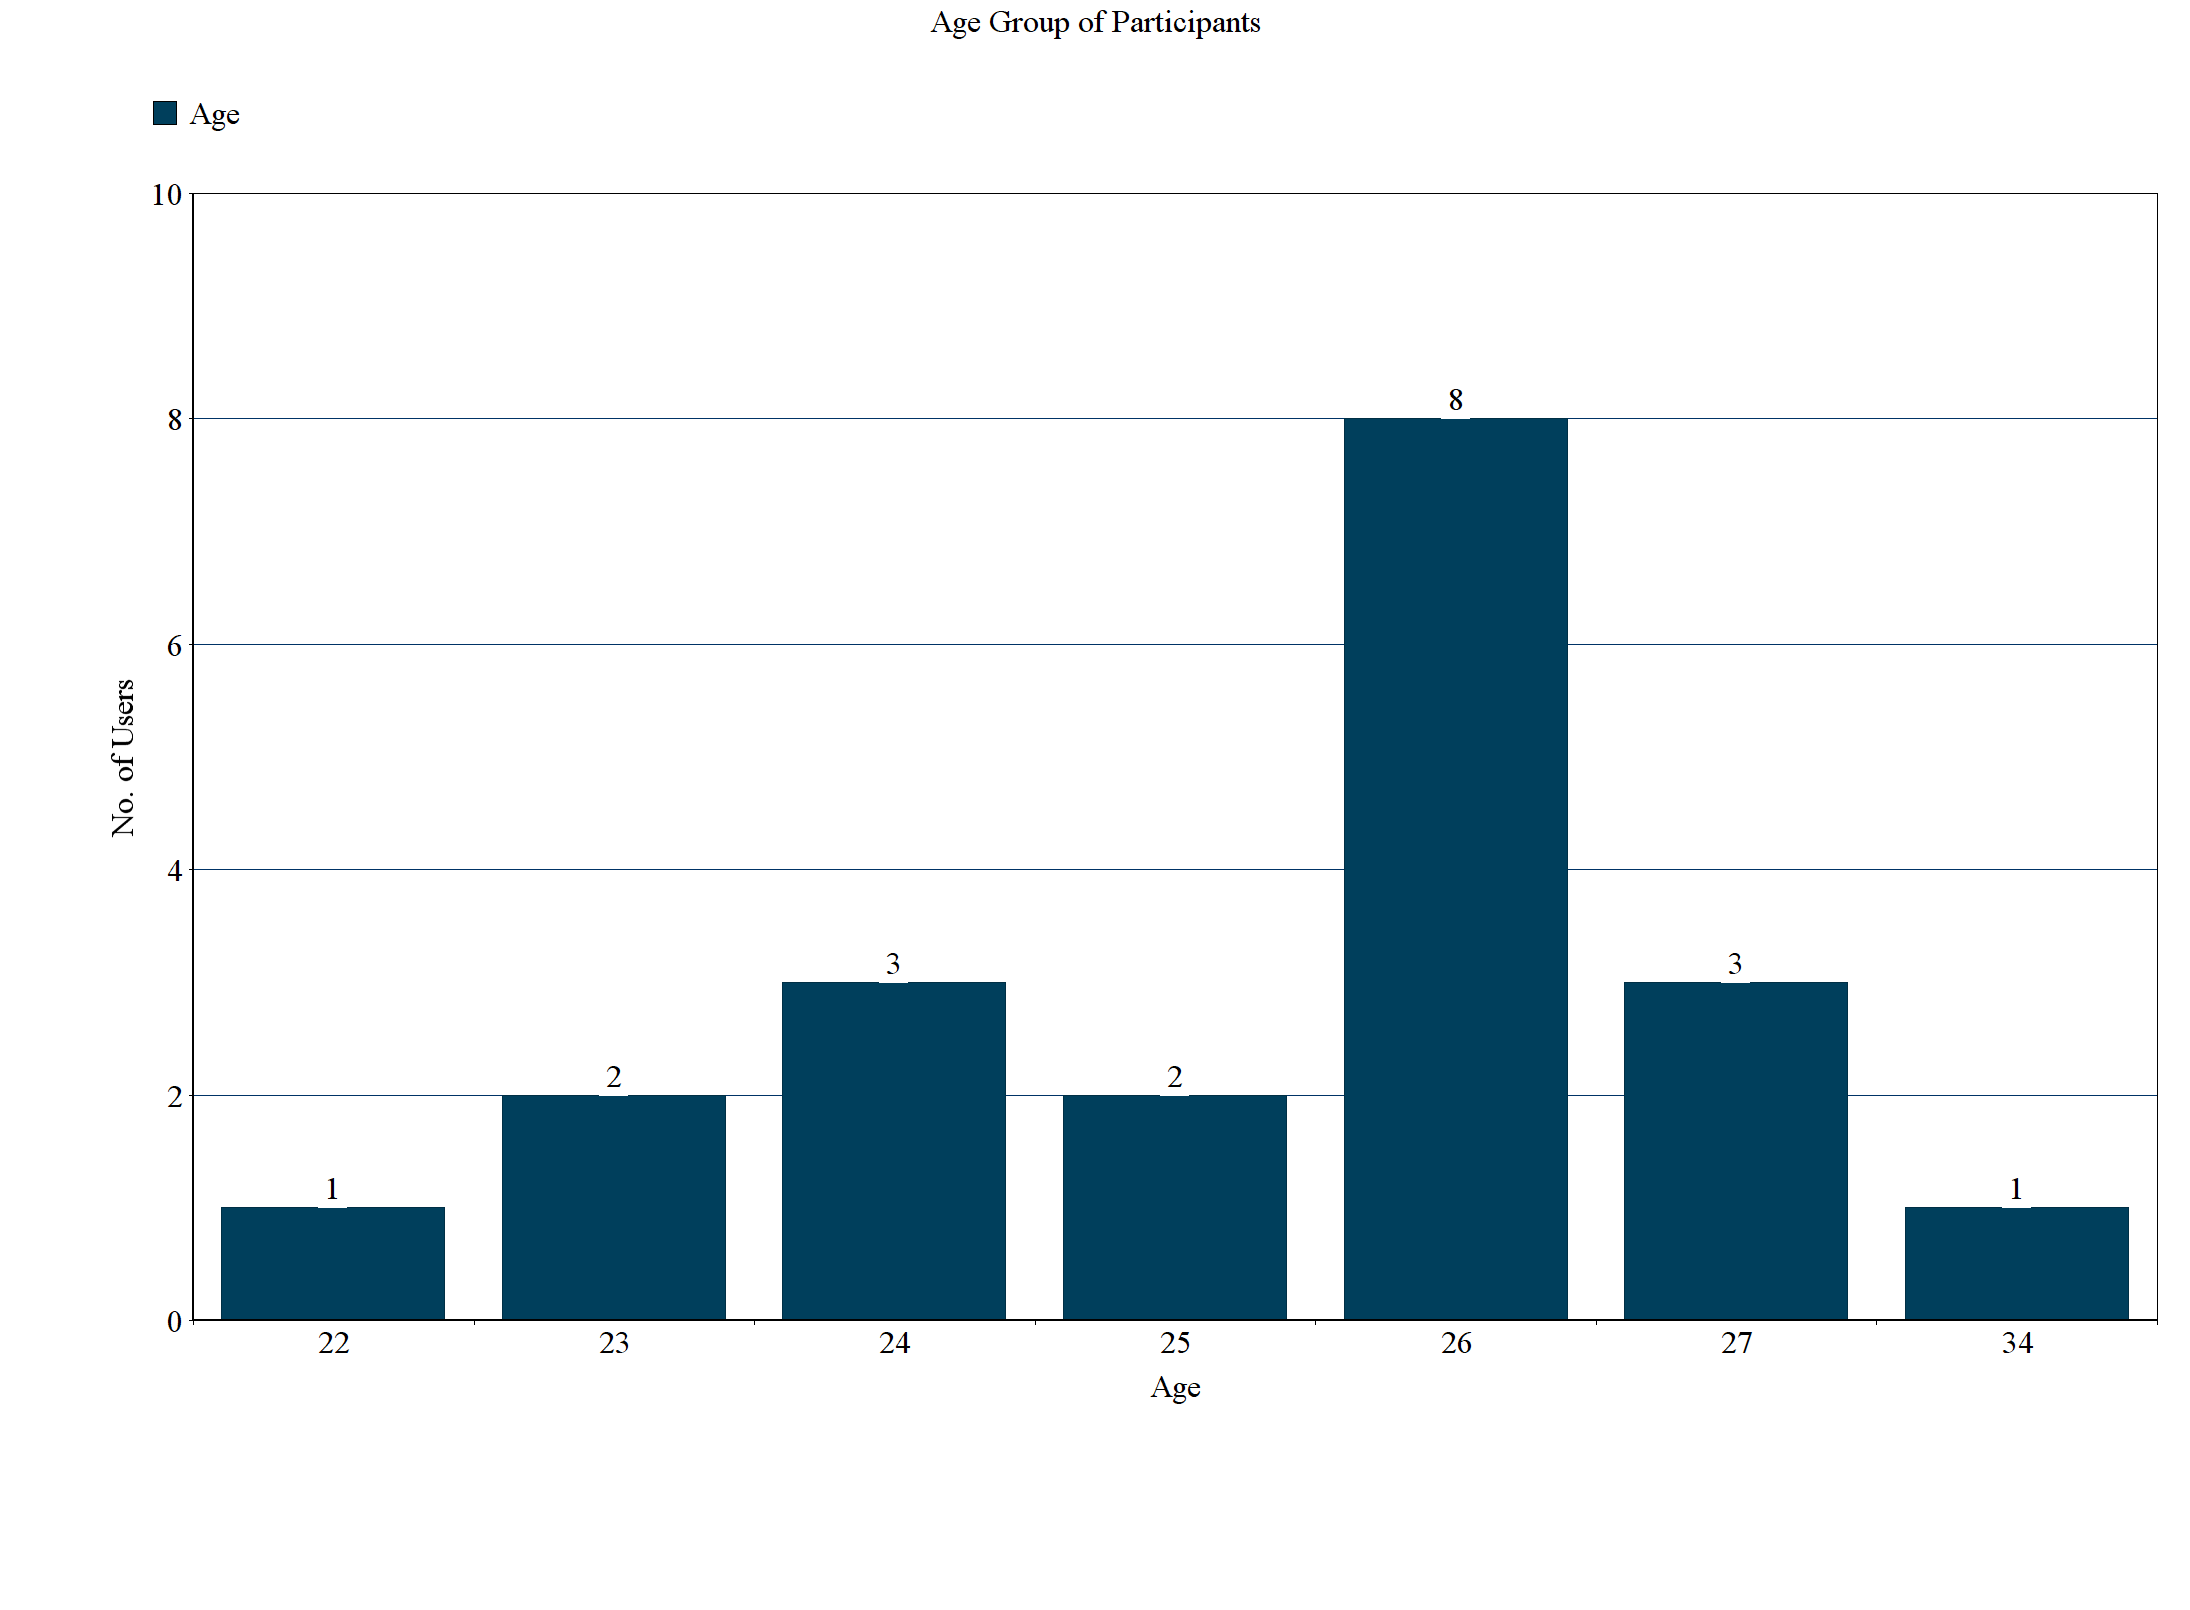
\includegraphics[width=0.9\textwidth]{img/Age_Graph_Updated.PNG}
    \caption{Age stats of participants}
    \label{fig:ageGraph}
\end{figure}
\\~\\
Figure \ref{fig:profGraph} depicts that total 20 users participated in this study. Most of them appeared to be from technical background as maximum of them appeared to be students from different universities. Second majority of participants revealed themselves as IT employees. While remaining revealed themselves as teacher and business qualified.

\begin{figure}[!h]
    \centering
    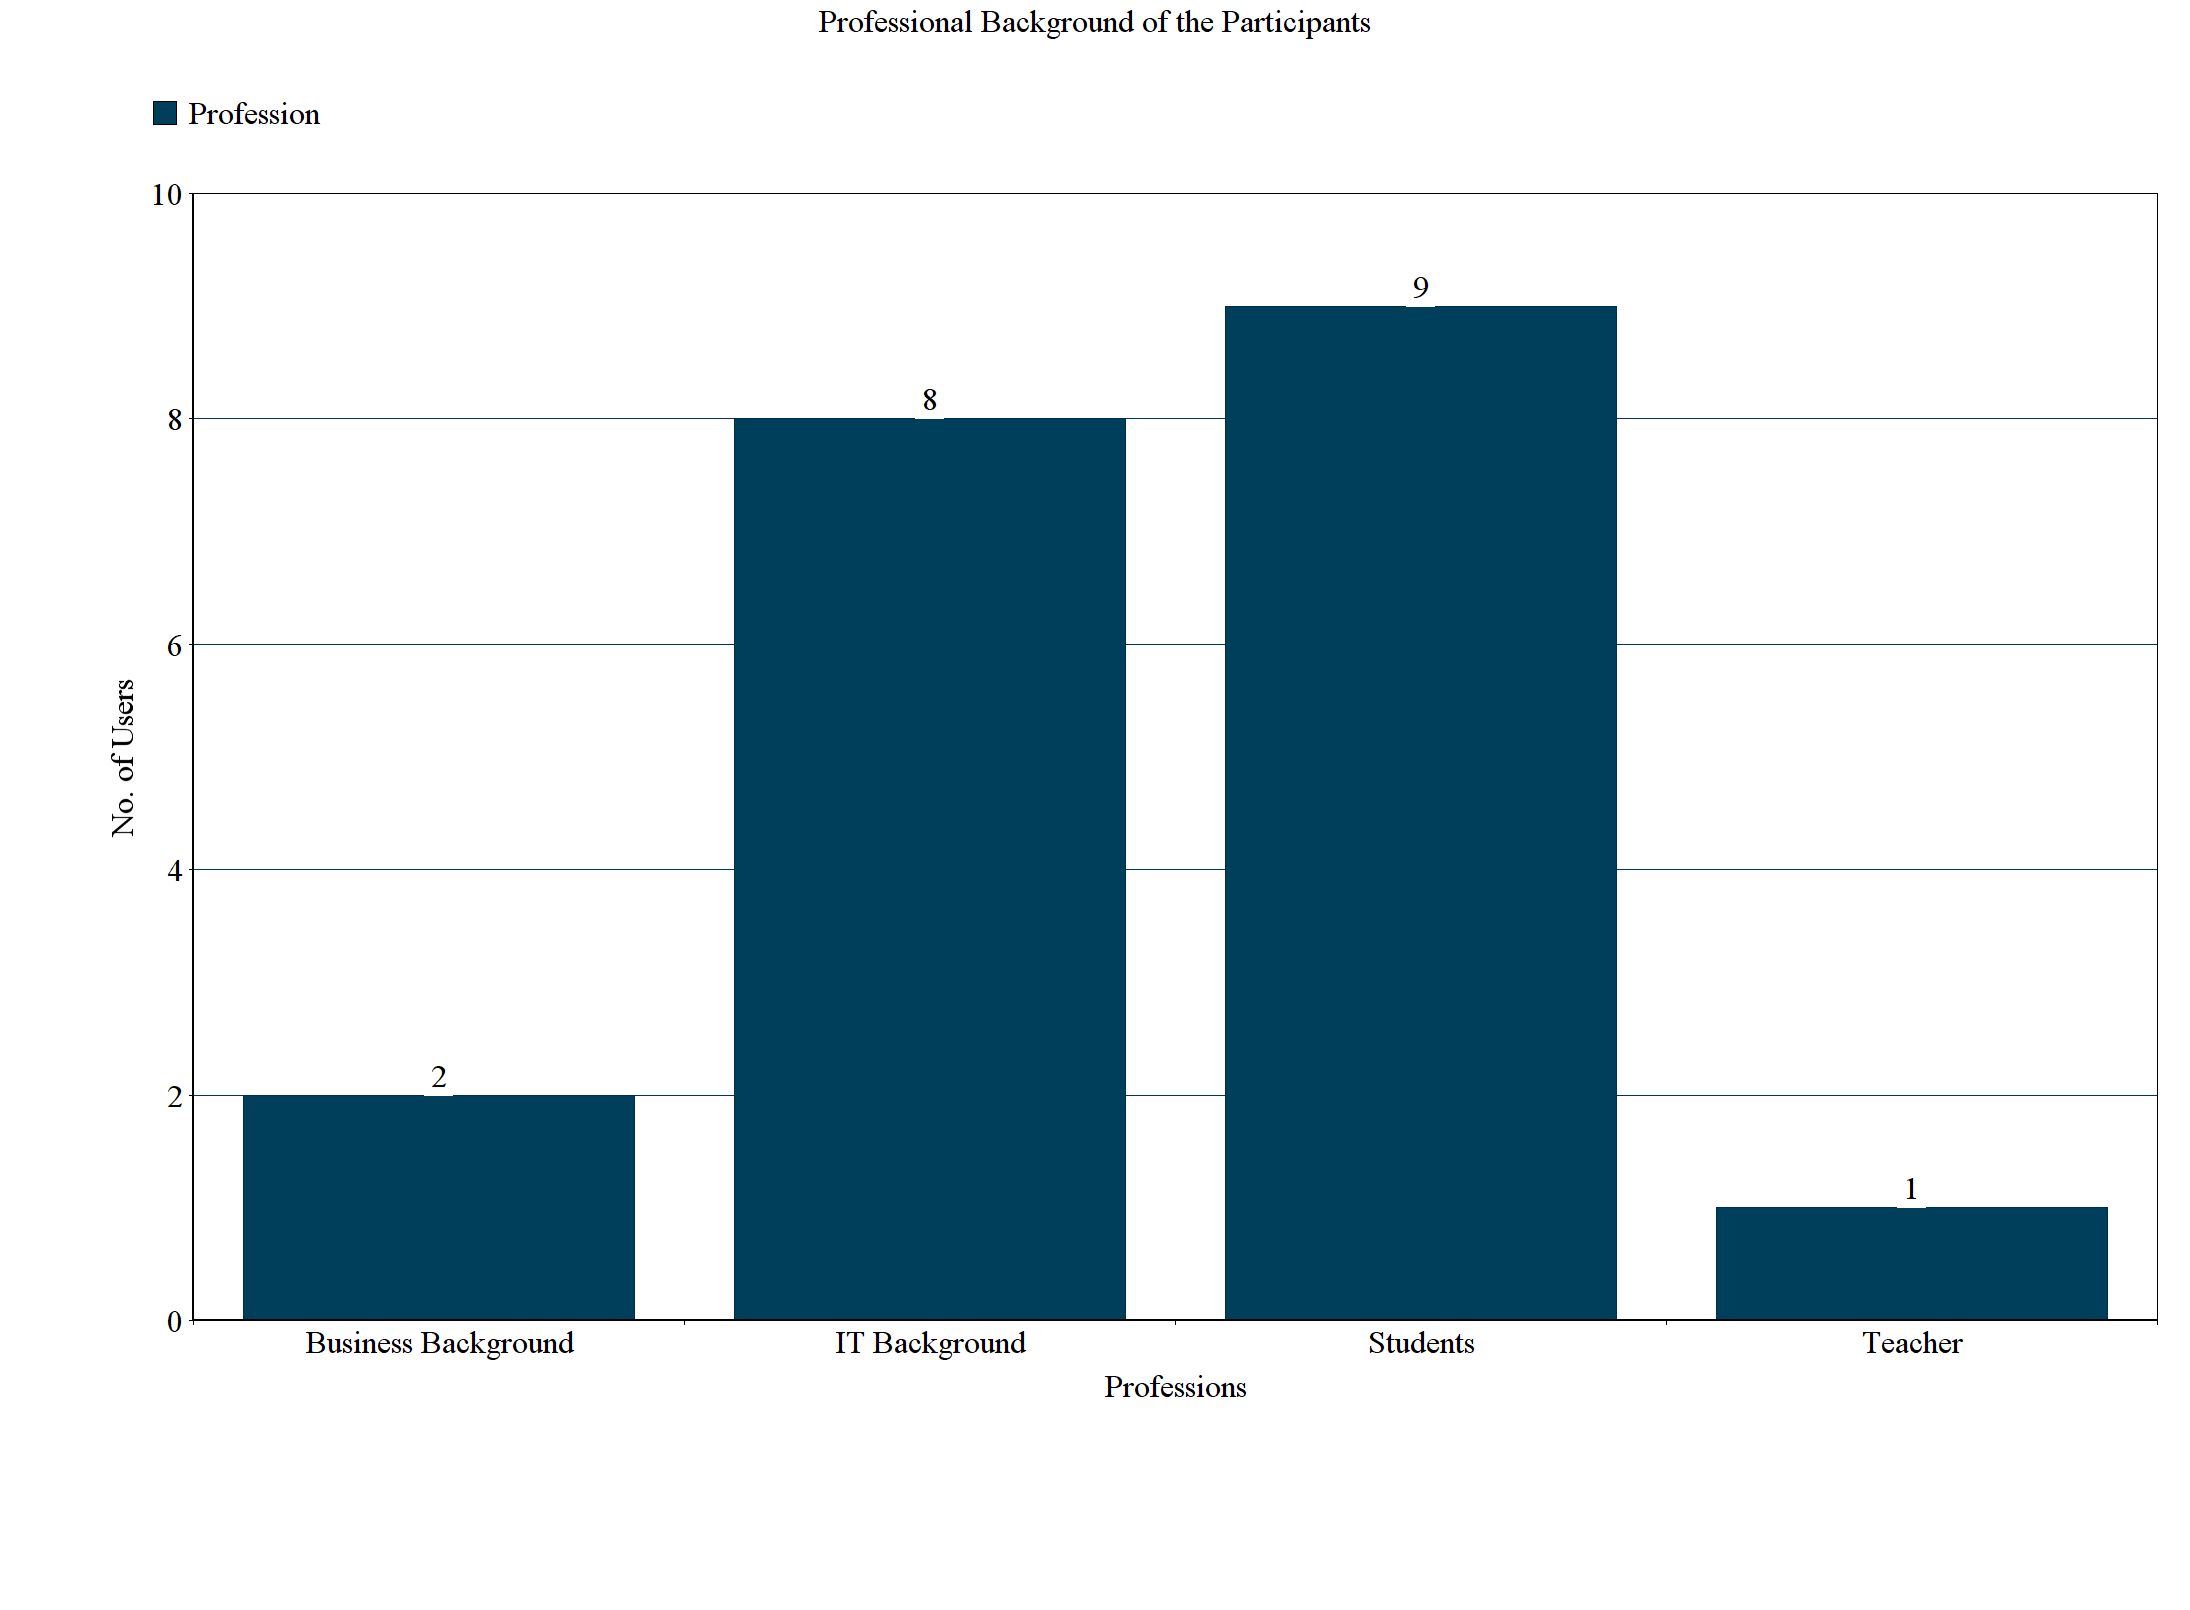
\includegraphics[width=0.9\textwidth]{img/Profession_Graph_Updated.PNG}
    \caption{Profession related details of participants}
    \label{fig:profGraph}
\end{figure}

\section{Conducted Surveys}
All participants were asked to complete two surveys. One named as "Frankenbot's Experience Survey" was designed with the help of \cite{evaluatingSpokDialSys}\cite{itut}. For the second survey, the standardized tool to personally evaluate the usability and design of an interactive product known as AttrakDiff \cite{attrakdiff} has been used. First survey was designed using Google Forms and the purpose of it was to capture the user's interaction experience about the Frankenbot. While, the purpose of AttrakDiff's study was to evaluate different aspects such as Frankenbot's utility and usability. Furthermore, it also helped to weigh the chatbot for task-oriented and self-oriented qualities. 
\\~\\
The users were provided with the link to the deployed chatbot's interface as a web page and they can easily access it from their own places. It provided ease to the user and enhanced the comfortability factor for them. Also, they have to read the description and instructions provided for them on the web page. And they have to figure out what to do and how to operate the chatbot on their own without any external help. Which has given more realistic and unbiased essence to the results obtained.
\\~\\
For the surveys, the web page contains the heading as "Frankenbot's Request" in which the users were requested to complete the surveys. Once, they are finished having chat for a fun purpose with the chatbot then they could visit the hyperlinks provided for both of the surveys.
\\~\\
The surveys were conducted in English language. Whereas, AttrakDiff's survey has the option for both English and German. You can find the "Frankenbot's Experience Survey" in the Appendix \ref{appen:survey}. Furthermore, AttrakDiff's Single Evaluation Study\cite{indeval} has been used as the second survey.
\\~\\
The questionnaires were filled by the participants on their own devices. While a user was interacting with the chatbot all communication was getting stored in to the log file for the future records and usage.

\section{Experimental Setup}
This research study has been conducted to gather the results for what user has experienced while interacting with the chatbot. The whole experiment itself has been divided in to four major parts mentioned below:
\begin{enumerate}
    \item Explanation of the chatbot for the participants in order to make its testing successful.
    \item Participants were requested for accomplishing set of tasks with the chatbot.
    \item The questionnaire to collect the user's interaction experience about the chatbot named as "Frankenbot's Experience Survey".
    \item Quality evaluation of the chatbot via AttrakDiff's Single Evaluation.
    \item Short interview of the participants.
\end{enumerate} 
All of these are explained underneath in detail.

\subsection{Explanation of the Chatbot}
Users were provided with the description and instructions on the web page about the chatbot. The following sub-sections contain the required information and directions to for the users to operate the chatbot. Visual representation has been displayed in the Figure \ref{fig:userInter}.

\subsubsection*{Information}
Real information provided to the participants has been provided in Appendix \ref{appen:info}. They were provided with the introduction about the Frankenbot that it is the detective chatbot designed to interrogate you about the armed robbery happened few days back at a spatkauf near Berliner Strasse. It is responsible for investigating, so it is going to ask you some questions to come up with a decision. It will include, what it has investigated so far. Also you can have general conversation with it like you can ask it to talk about general stuff with you, about corona virus and its stats, to make you laugh, to do gossips, how does it feel, who is it, what does it eat and other related questions about the chatbot. You can switch between the topics at any moment as it is designed for parallel handling of the multiple topics. Kindly, communicate with it until it reaches any decision or says you goodbye before you jump to completion of the surveys.
\\~\\
Lastly, the ending of the information provided a brief note about how to re-initiate the chat. If user gets lost in between the dialogue and want to reinstate the detective game then just send a greeting message (hi, hello etc.) and the chatbot will restart it for him/her. 

\subsubsection*{Instructions}
Actual instructions are stated in Appendix \ref{appen:instr}. The user was asked to think as he/she is accused of a robbery and sitting in front of a detective and have to answer his deceptive questions in order to prove his/her innocence. Otherwise, he/she will be declared as a culprit. It is a responsibility of a detective to make a decision based on the user's answers to his questions.
\\~\\
At the end of the instructions there was a small notice available for the user to remove his/her doubts about its reality that it is the fictional detective chat bot designed only for testing and fun purpose.

\subsection{Tasks}
The participants were requested to accomplish following tasks beforehand, to fill the surveys.
\begin{itemize}
    \item Users were requested to play a small game with the detective chatbot and answer the questions, the way they wanted.
    \item They were also informed that they could have general dialogue with the chatbot. They could also talk to it about general stuff, corona virus and its stats, to tell a joke, to do gossips, query about its feelings and emotions and other related questions.
    \item Additionally, they were also notified that they are able to switch the topics. Means, they can start talking about general stuff if they are talking to the detective bot and vice versa by just replying to the last question of the previous topic.
    \item Lastly, they were requested not to leave the conversation in between until they reach the ending of the detective game. 
\end{itemize} 
\\~\\
All users were requested to chat with the chatbot at minimum, until it came up with any decision or says them goodbye. Other than that, there was no time restriction for them and they could have a dialogue for as long as they desired to.

\subsubsection*{Frankenbot's Request}
Finally, the user was requested as stated in Appendix \ref{appen:req} that once he/she has finished interaction with the chatbot, please don't forget to complete two of the assessments demonstrated in Appendix \ref{appen:survey}. They were allowed to start with it after 1 minute of web page activation at minimum. Meanwhile, a user should get familiar with the chatbot by chatting with it. Frankenbot also stated that it welcomes and highly appreciates the user's prestigious feedback which will help its developer to get it evaluated and enhance its abilities for better experience.

\subsection{Interview\label{subsec:interview}}
At the end, a brief interview was conducted after having their consent. And not all the users gave permission for it but 12(60\%) of the participants showed their availability for a small session. The users have been verbally asked the following questions:
\begin{itemize}
    \item Whether they faced any problem to make chatbot understand their messages?
    \item Did they reach the end of detective game i.e. a chatbot declared them culprit or responded them with bye message?
    \item Whether chatbot guided them well in case of any confusion that how to proceed ahead?
    \item Did they enjoy the communication?
    \item Did they try with switching the topics?
    \item Whether they liked the detective game or not?
    \item Whether they liked the user interface or not?
\end{itemize}

\subsection{Frankenbot's Experience Questionnaire}
When the user successfully completed the tasks allocated to him/her then he/she filled out the questionnaire about his/her interaction with the chatbot. The questionnaire shown in Appendix \ref{appen:expsurvey} has been divided in to the following sections:
\begin{itemize}
    \item Users overall impression about the interaction with the chatbot.
    \item Familiarity of the user with the already existing chatbots.
    \item Whether the user succeeded to achieve the desired goals.
    \item How was the communication with the chatbot.
    \item What was the behaviour of the chatbot with the users.
    \item How well the dialogue was designed.
    \item Personal impression and user's experience about the chatbot.
    \item Users opinion about the chatbot's usability. 
\end{itemize} 
All sections have been consisted of several questions. And user has to respond by selecting an option out of linear scale from 1 to 5 whether he/she strongly agrees, agrees, undecided, disagrees or strongly disagrees with it. Most of the questions needed to be answered using these five options. Other than that overall impression about the chatbot has been measured using the linear scale of 5 options starting from 1 and ending on 5 as excellent, good, fair, poor and bad.

\subsection{AttrakDiff Single Evaluation}
After completing the Frankenbot's Experience Survey, users have been requested to complete the AttrakDiff's standardized questionnaire to measure that how the users perceived the design, quality and usability of the chatbot.
\\~\\
The AttrakDiff is an institutional questionnaire that has been used to rate the products using the series of several word pairs \cite{alex}. Each word pair consists of the options as a linear scale from 1 to 7. Option at position 1 is a word while on number 7 there also exists a word but its acronym \cite{attrakdiffQuest}. These pairs of the words are classified into three following categories: (i) Pragmatic Quality, it includes the word pairs like “cumbersome - straight forward” and “impractical - practical”. (ii) Hedonic Quality, the words pairs like “tacky - stylish” and “unimaginative - creative” lies under this category. And (iii) Attractiveness, word pairs such as “pleasant - unpleasant” and "ugly - attractive" are grouped under this attribute \cite{alex}.

\section{Quantitative Analysis}
This section contains the explanation and quantitative analysis of the results obtained during the research. It has been further divided in to two steps: (i) The results for all the sections for the Frankenbot's Experience Survey as mentioned above and also the results for the AttrakDiff Single Evaluation stated before. 

\subsection{Frankenbot's Experience Survey}
It analyzes the results gathered about all the sections of the questionnaire.

\subsubsection*{Overall Impression}
This section includes a question about the user's overall impression about the interaction with the chatbot as pictured in Figure \ref{fig:overallImpre}. It has been measured using the linear scale of 5 options starting from 1 and ending on 5 as excellent, good, fair, poor and bad. And out of the total 20 responses collected by the conduction of the survey, 2(10\%) responded with excellent mark and 9(45\%) rated it as good. So, total 11 out of 20 which is 55\% of the total participants, have passed positive remarks about it. Whereas, other 4(20\%) judged it as fair which also lies under the category of acceptable. So after summing up the percentages, 75\% of the participants rated their interaction as charming. On contrary, out of the remaining participants 3(15\%) rated it as poor and only 2(10\%) assigned it a bad label. So, it depicts that overall users impression about the interaction with the chatbot went well.

\begin{figure}[!h]
    \centering
    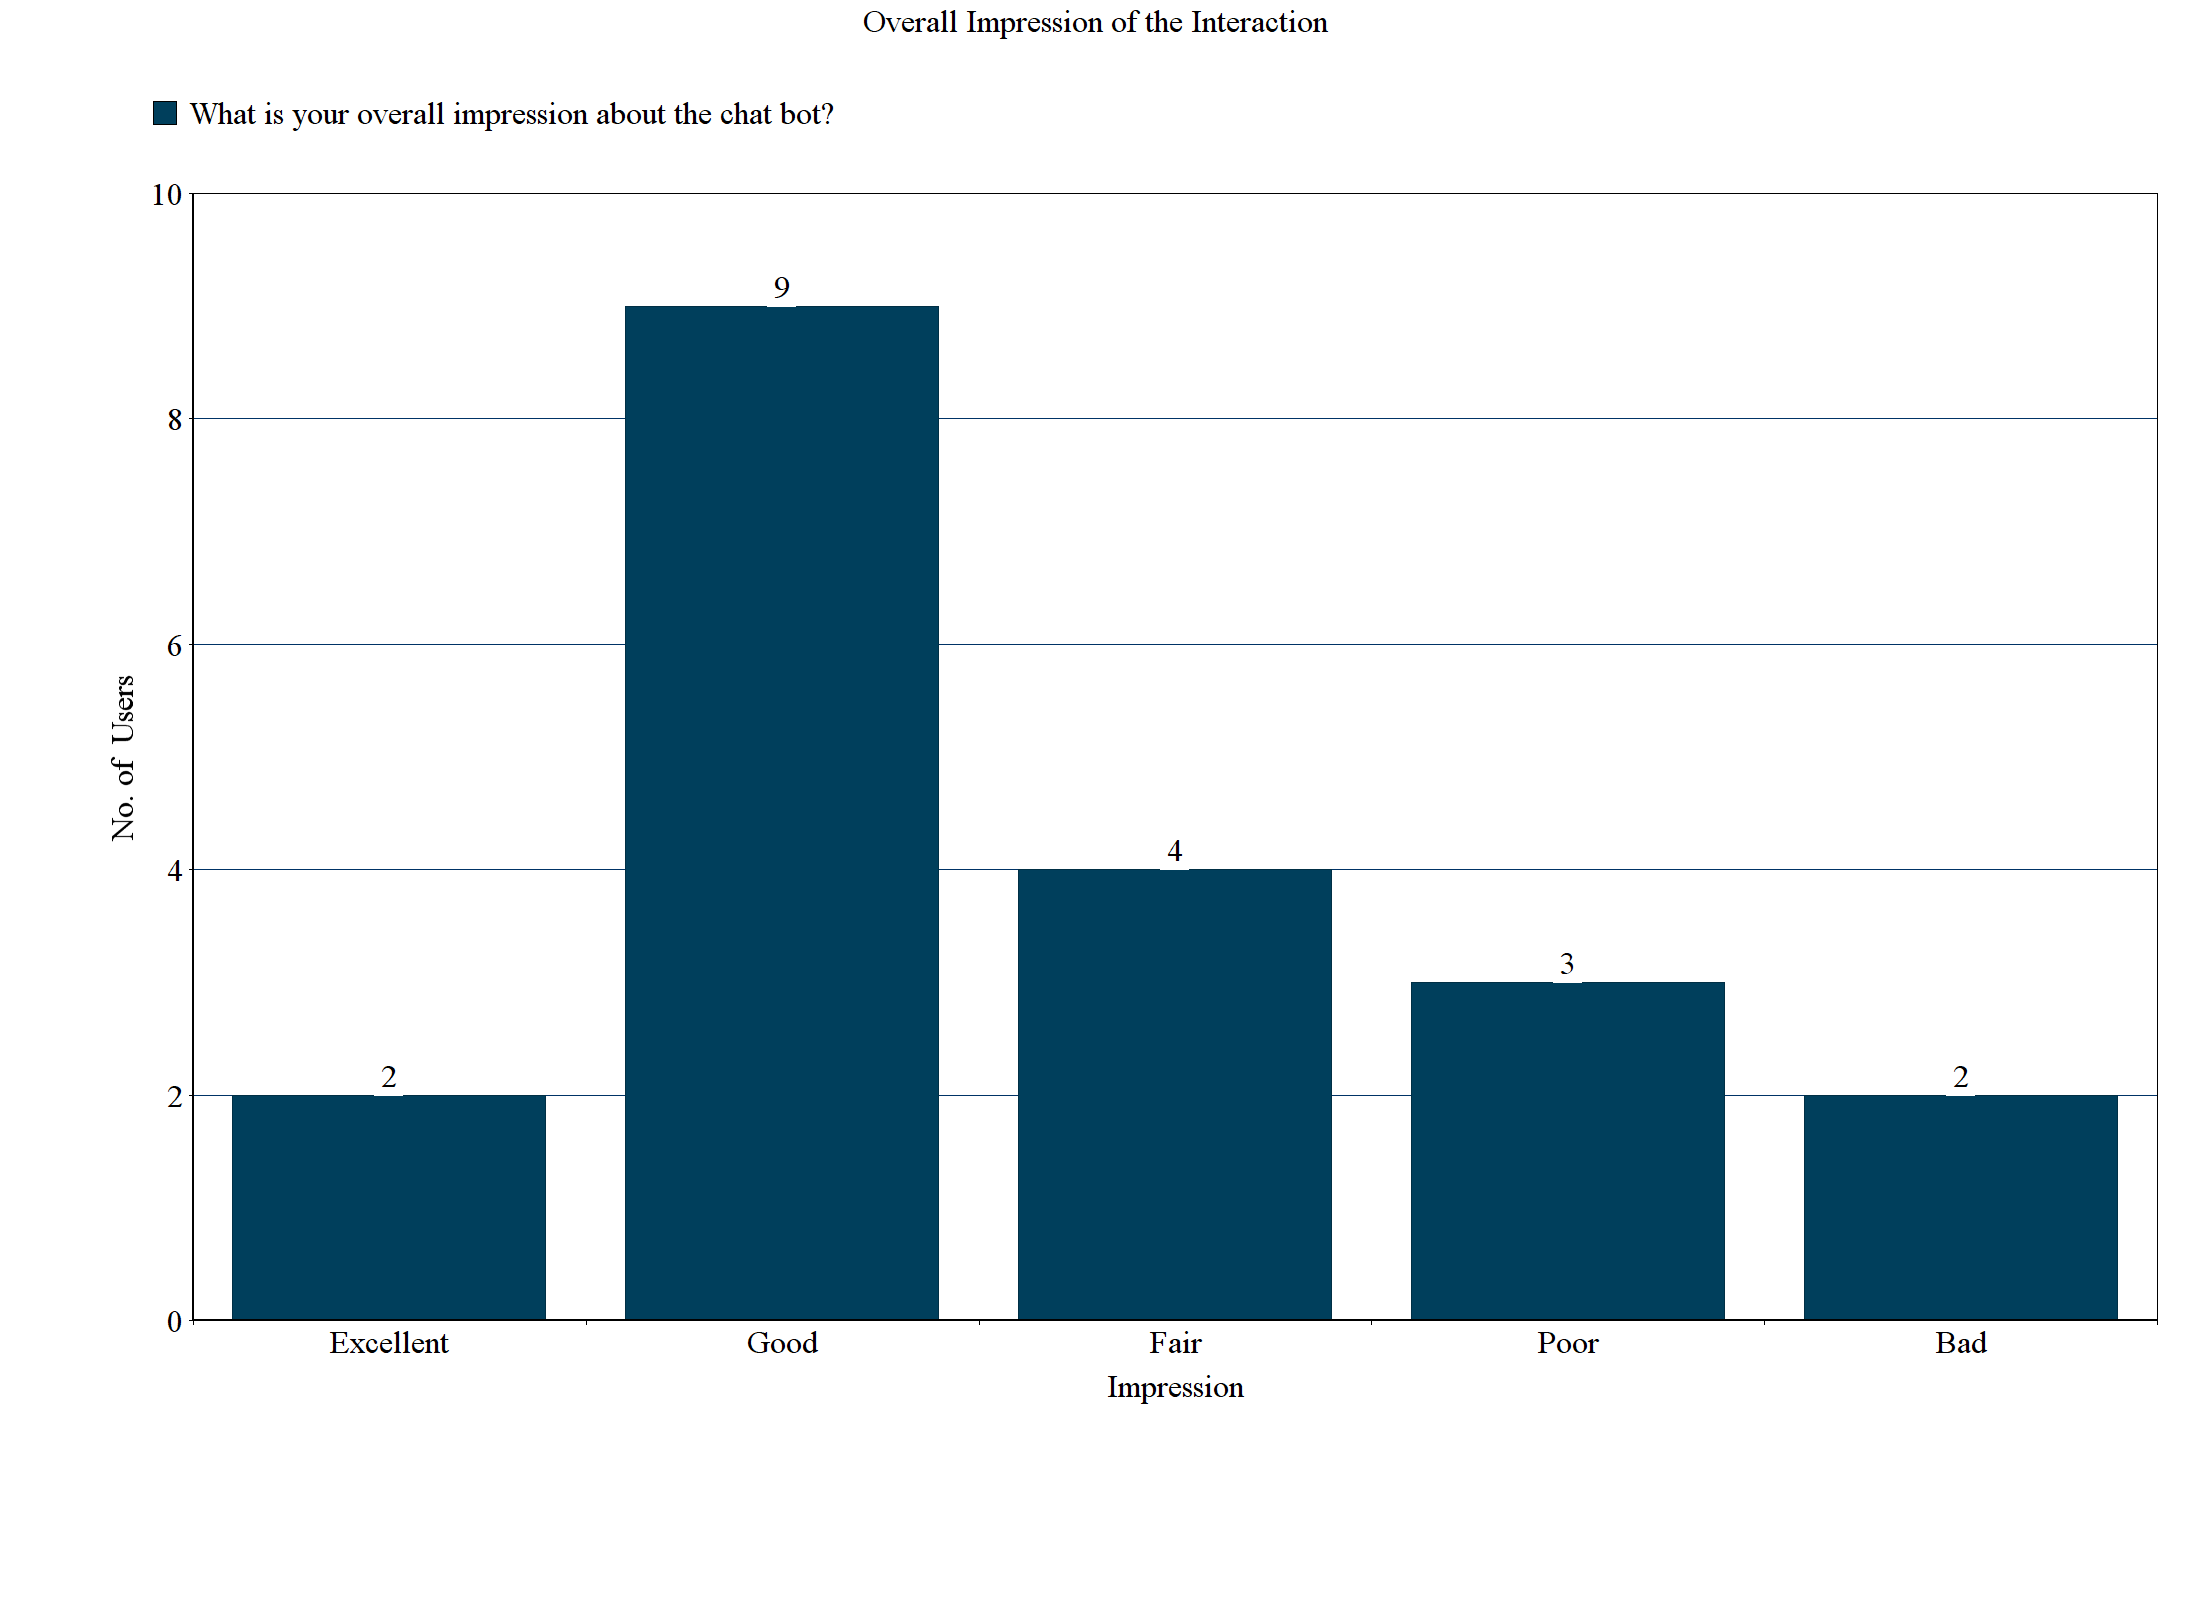
\includegraphics[width=0.9\textwidth]{img/Overall_Impression_Updated.PNG}
    \caption{Overall impression of the interaction with the chatbot}
    \label{fig:overallImpre}
\end{figure}

\subsubsection*{Familiarity with Existing Chat Bots}
This section added to the questionnaire just to figure out the experience of the participants with already existing chatbots. Whether they were well familiar with the chatbots or are inexperienced with this emerging technology. So that if majority of them have the good knowledge of any of the existing chatbots, it will provide more strength and solidity to the results gathered from such participants.
\\~\\
There were total 3 questions available under this section of the survey attached in Appendix \ref{appen:expsurvey} that participants have to answer:
\begin{enumerate}
    \item I feel that I am well familiar with the chat bots like Google Assistant, Apple's Siri etc. (Possible options lie between scale of strongly agree to strongly disagree).
    \item I communicate with the chat bots. And the possible options provided were Frequently (daily or several times in a week), Seldomly (rarely in weeks or months), Just few times and Never.
    \item Purpose of my chat bots usage is: (only if you answered question no. 2 positively). Possible answers could be any out of the followings: Personal commands to provide you assistance in performing tasks, For fun, Not feel lonely and No reason.
\end{enumerate}
Fortunately, for the first statement, 16(80\%) appeared to be well familiar with the existing chatbots. 2(10\%) answered with undecided and remaining 2(10\%) just disagreed with the statement but no one strongly disagreed with it. Graph depicting such results has been shown in the Figure \ref{fig:familiarity}. Coming to the second statement, 5(25\%) detected to be frequent users. 8(40\%) resulted to be the seldom users. Whereas, 6(30\%) communicated just few times with the chatbots as shown in the Figure \ref{fig:commChatRes}. Lastly, almost 60\% knew how to operate and give commands to the chatbot. And around 30\% appeared to use it for joy and fun purpose. These all stats and readings portrays that experienced users participated in this study. And results obtained from the study is trustworthy and reliable. 

\begin{figure}[!h]
    \centering
    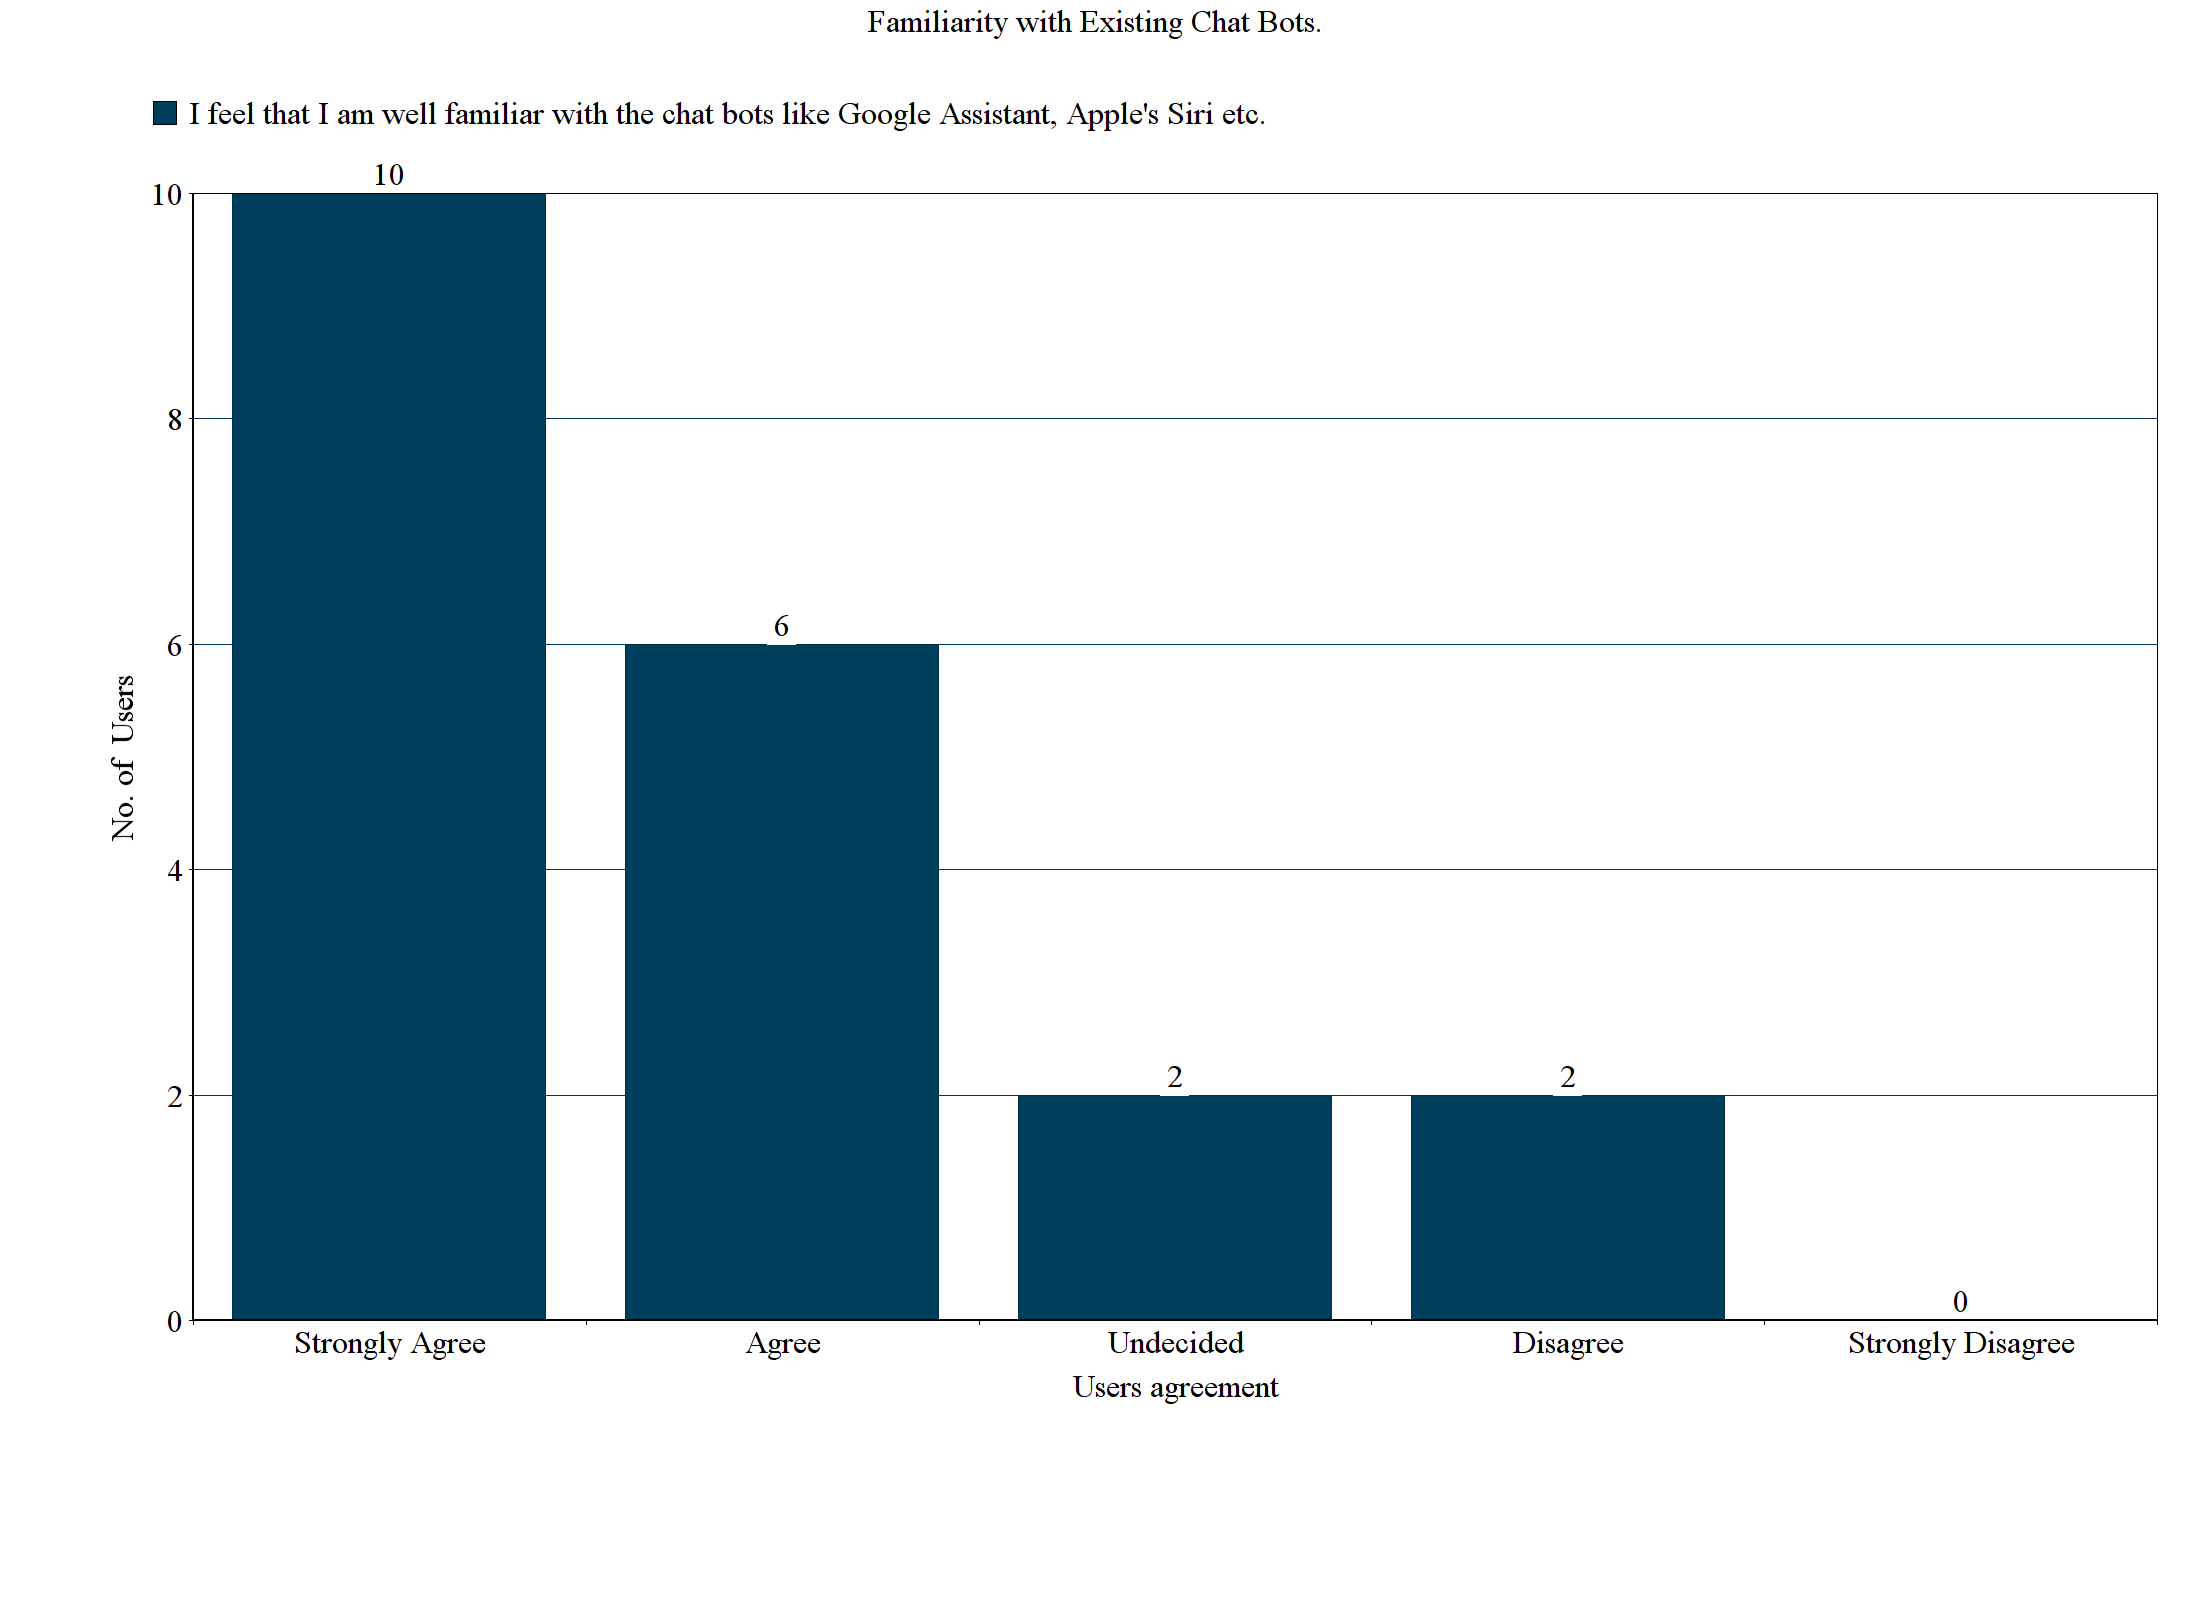
\includegraphics[width=0.9\textwidth]{img/Familiraity_Updated.PNG}
    \caption{Participants familiarity with the chat bots like Google Assistant, Apple's Siri etc.}
    \label{fig:familiarity}
\end{figure}

\begin{figure}[!h]
    \centering
    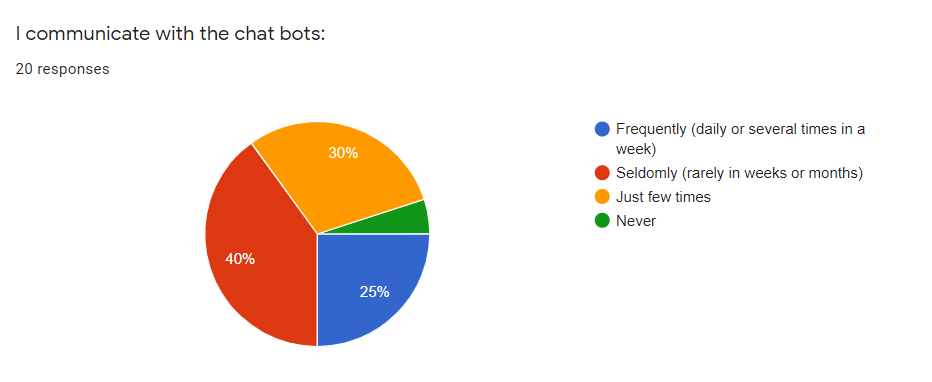
\includegraphics[width=0.9\textwidth]{img/Communicate_Chatbots_Result.PNG}
    \caption{Participants usage of the chat bots like Google Assistant, Apple's Siri etc.}
    \label{fig:commChatRes}
\end{figure}

\subsubsection*{Achievement of Goals}
It highlights whether the user succeeded to achieve the desired goals or not while having an interaction with the chatbot. It contained the following questions in respond to which user checked an option that varied from strongly agree to strongly disagree. Detailed comparison for all the answers collected for the following statements can be found in the Figure \ref{fig:achievGoals}.
\begin{enumerate}
    \item The information provided by the chat bot was clear.
    \item The provided information was incomplete.
    \item The interaction with the chat bot was efficient.
    \item The chat bot is unreliable.
\end{enumerate}

\begin{figure}[!h]
    \centering
    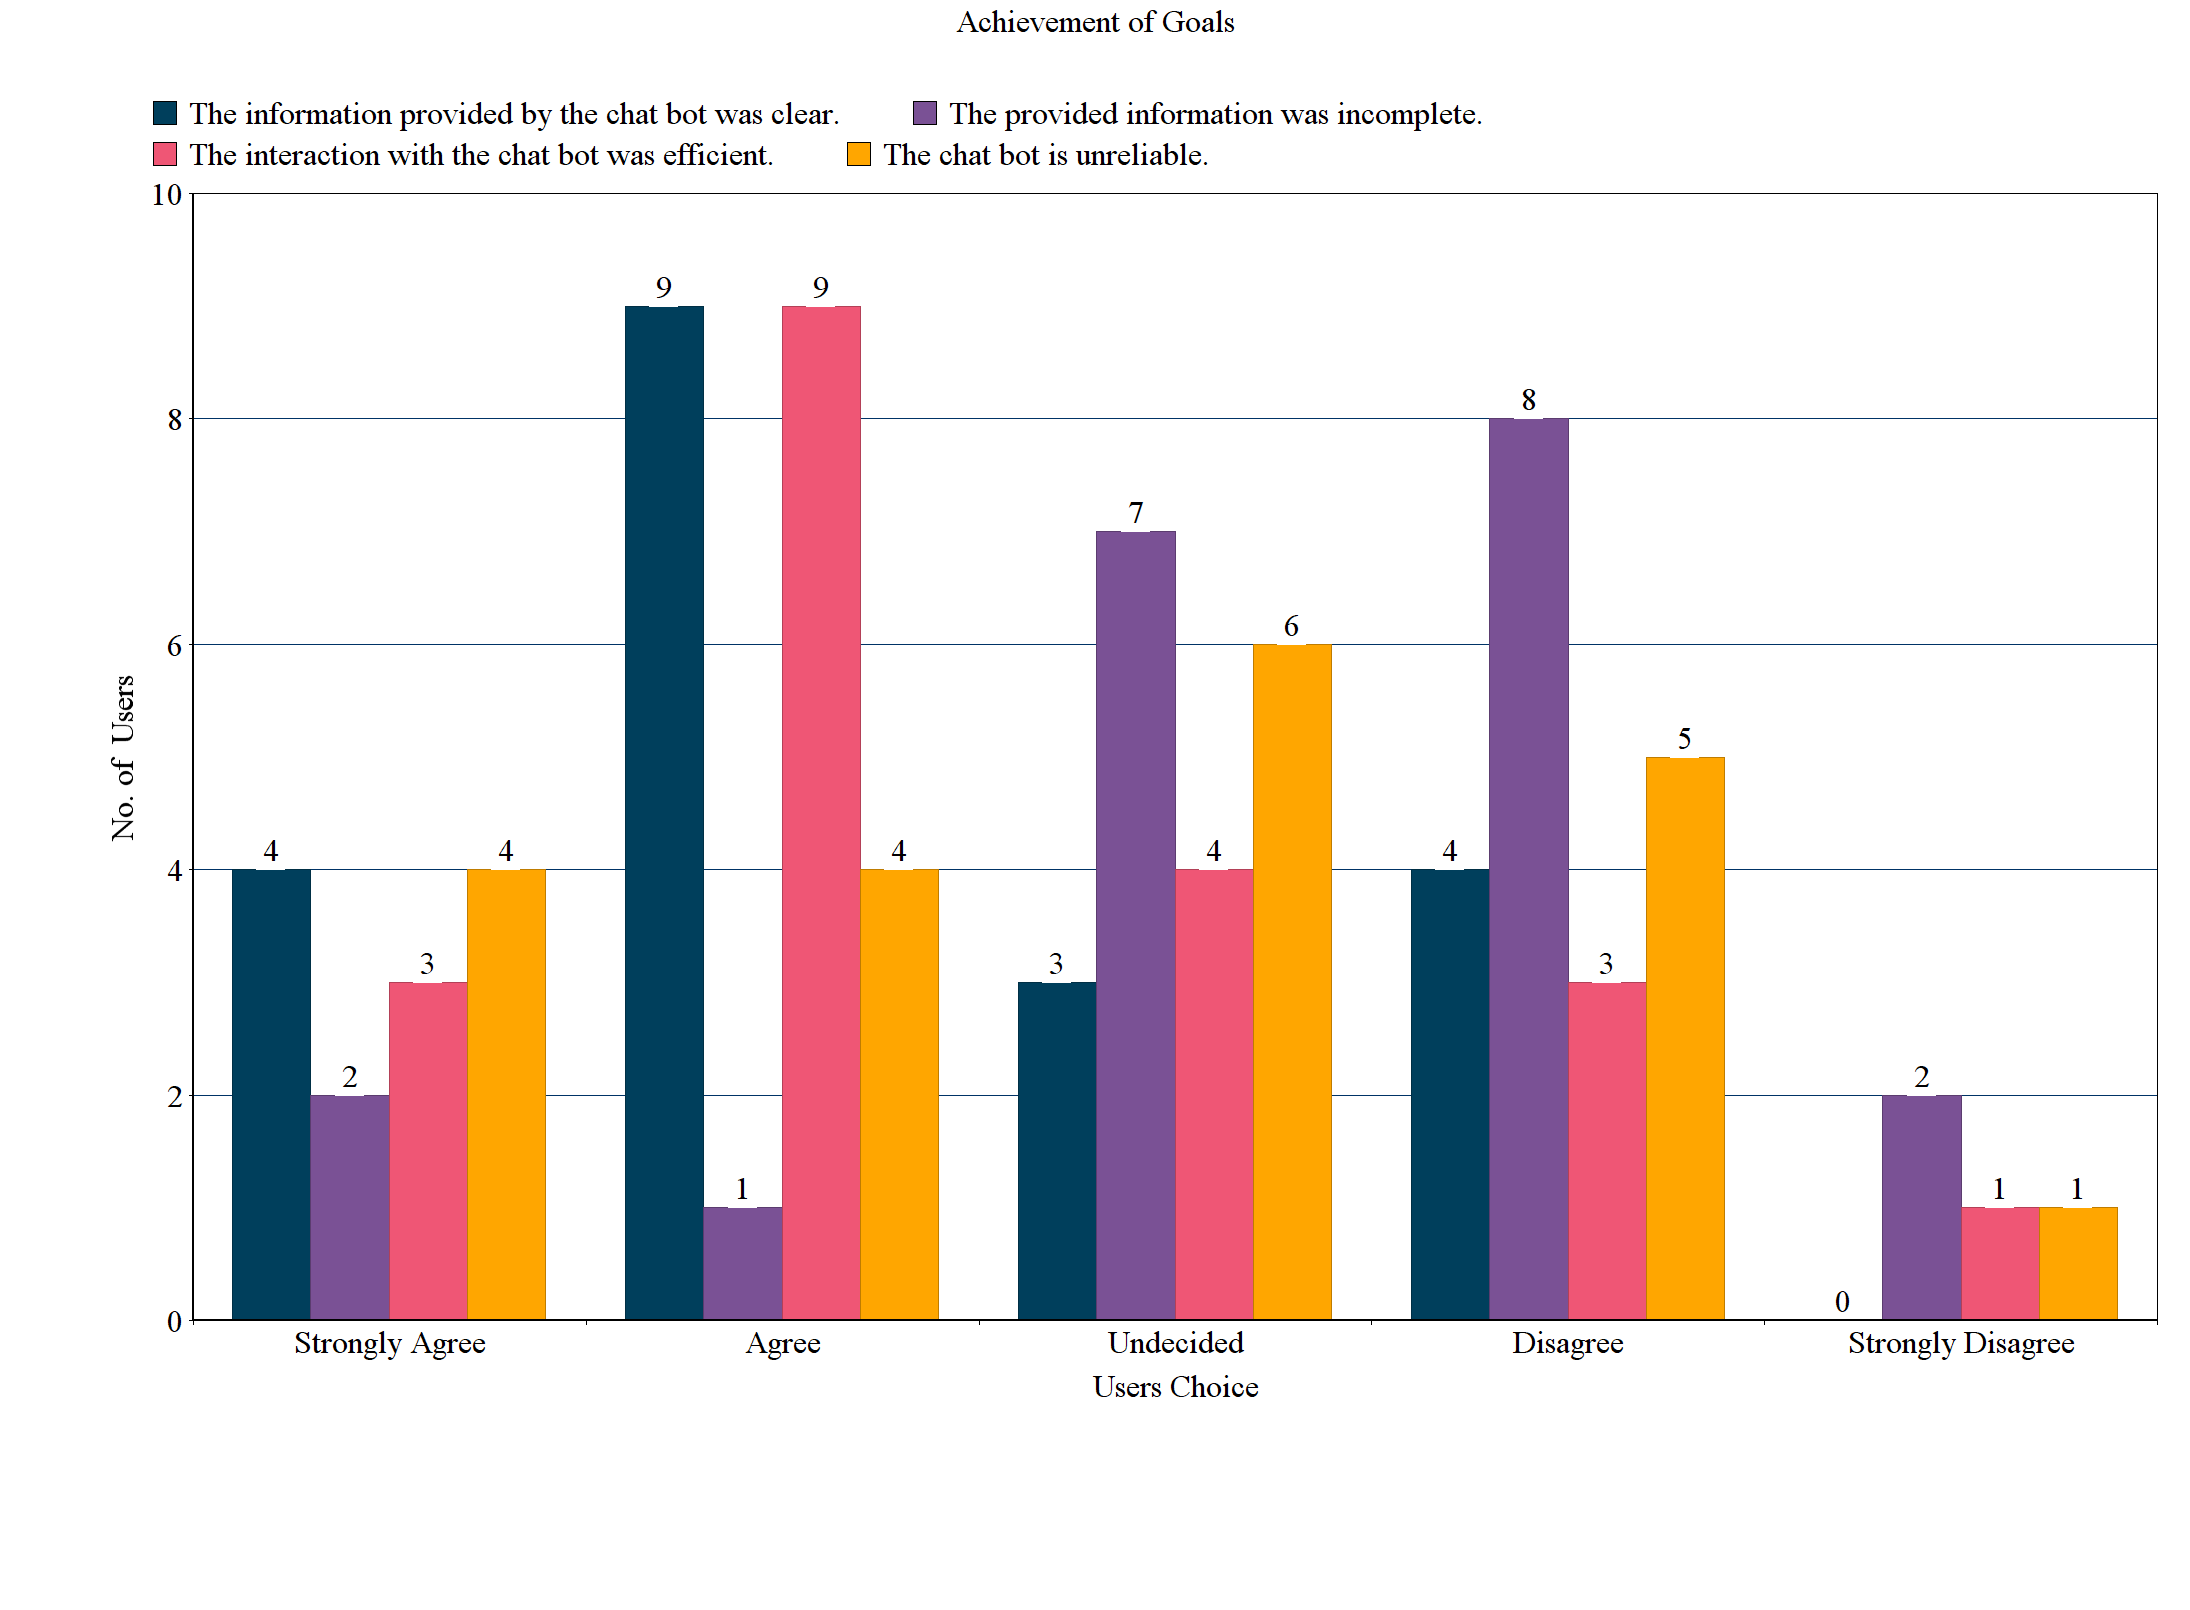
\includegraphics[width=0.9\textwidth]{img/Achievement_of_Goals_Updated.png}
    \caption{Graphical representation of collected responses for achievement of goals.}
    \label{fig:achievGoals}
\end{figure}
\\~\\
Discussing the results and stats for the very first statement, 13(65\%) participants agreed upon the information provided by the chatbot was clear. Whereas, 3(15\%) were failed to decide about it. Only 4(20\%) just disagreed with it and no one strongly negated it. For better understanding of it just see the Figure \ref{fig:achievGoals}.

% \begin{figure}[!h]
%     \centering
%     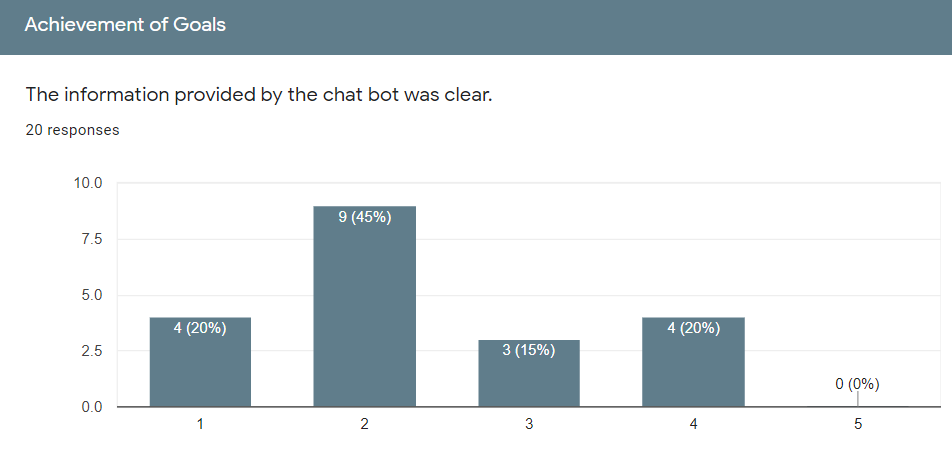
\includegraphics[width=0.9\textwidth]{img/Clear_Info.PNG}
%     \caption{Stats depicting about the information provided by the chat bot was clear}
%     \label{fig:clearInfo}
% \end{figure}
\\~\\
For the second statement, 10(50\%) disagreed with it which tells that for them the provided information was complete. Whilst 7(35\%) were unable to make any decision about it. This is something can not ignored. It can happen due to various reasons: (i) due to lack of concentration (ii) misinterpretation of information or instructions (iii) chatbot responded falsely and a reason for it could be a weakly trained Rasa's NLU due to limited training data as already mentioned before. But still 50\% answered that the information was complete, so there are high chances that the reason lies somewhere between (i) and (ii). Visuals have been shown in the Figure \ref{fig:achievGoals}.

% \begin{figure}[!h]
%     \centering
%     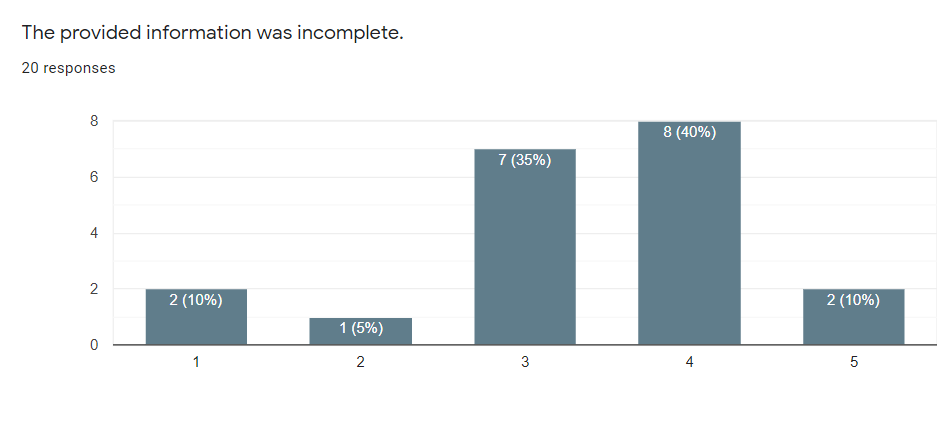
\includegraphics[width=0.9\textwidth]{img/Incomp_Info.PNG}
%     \caption{Stats depicting about the provided information was incomplete}
%     \label{fig:incompInfo}
% \end{figure}
\\~\\
Moving to what has been concluded from the third statement seems to be something really positive. As 12(60\%) of the participants agreed upon the efficient interaction with the chatbot. Moreover, 4(20\%) failed to decide about it and only other remaining 4(20\%) disagreed with it. Refer to the Figure \ref{fig:achievGoals} for better understanding by visuals.

% \begin{figure}[!h]
%     \centering
%     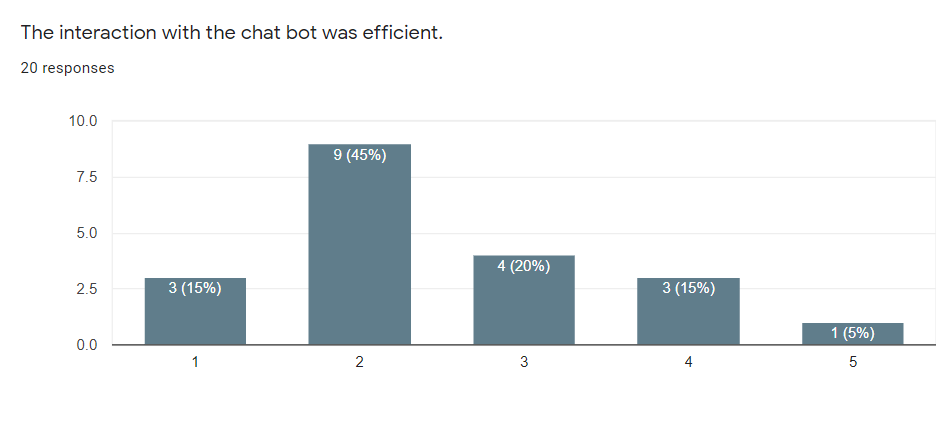
\includegraphics[width=0.9\textwidth]{img/Efficient_Inter.PNG}
%     \caption{Stats depicting about the interaction with the chat bot was efficient}
%     \label{fig:effInt}
% \end{figure}
\\~\\
Lastly, forth statement stats are a bit disappointing. According to only 6(30\%) users, the chatbot was reliable. On contrary, 8(40\%) declared it unreliable and remaining 6(30\%) failed to take any decision about it. The possible reason for its unreliability could be its inability to respond the user for all of his/her queries. And it happened due to limited data provided for training and also the demo chatbot was designed for limited use cases. In order to design a fully loaded chatbot that can reply to the user for any of his/her utterance, lot of training data and processing is required and within limited time and resources it was not possible. But, it could be done in future. See the Figure \ref{fig:achievGoals} for better visualization of the results.

% \begin{figure}[!h]
%     \centering
%     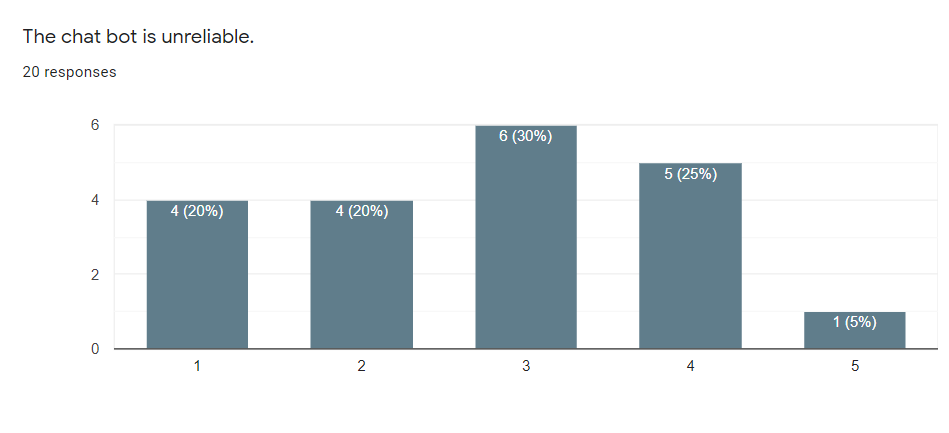
\includegraphics[width=0.9\textwidth]{img/Unreli_Bot.PNG}
%     \caption{Stats depicting about the chat bot is unreliable}
%     \label{fig:unreliBot}
% \end{figure}

\subsubsection*{Communication with the Chat Bot}
The purpose of this section was to collect the user's opinion that how was the communication with the chatbot. It consisted of the following three questions:
\begin{enumerate}
    \item The chat bot understood my messages well.
    \item I always knew what to say to the chat bot.
    \item The interaction with the chat bot sounded natural.
\end{enumerate}
Graphical representation for the detailed analysis and comparison of the results for these statements has been shown in the Figure \ref{fig:communwithBot}.

\begin{figure}[!h]
    \centering
    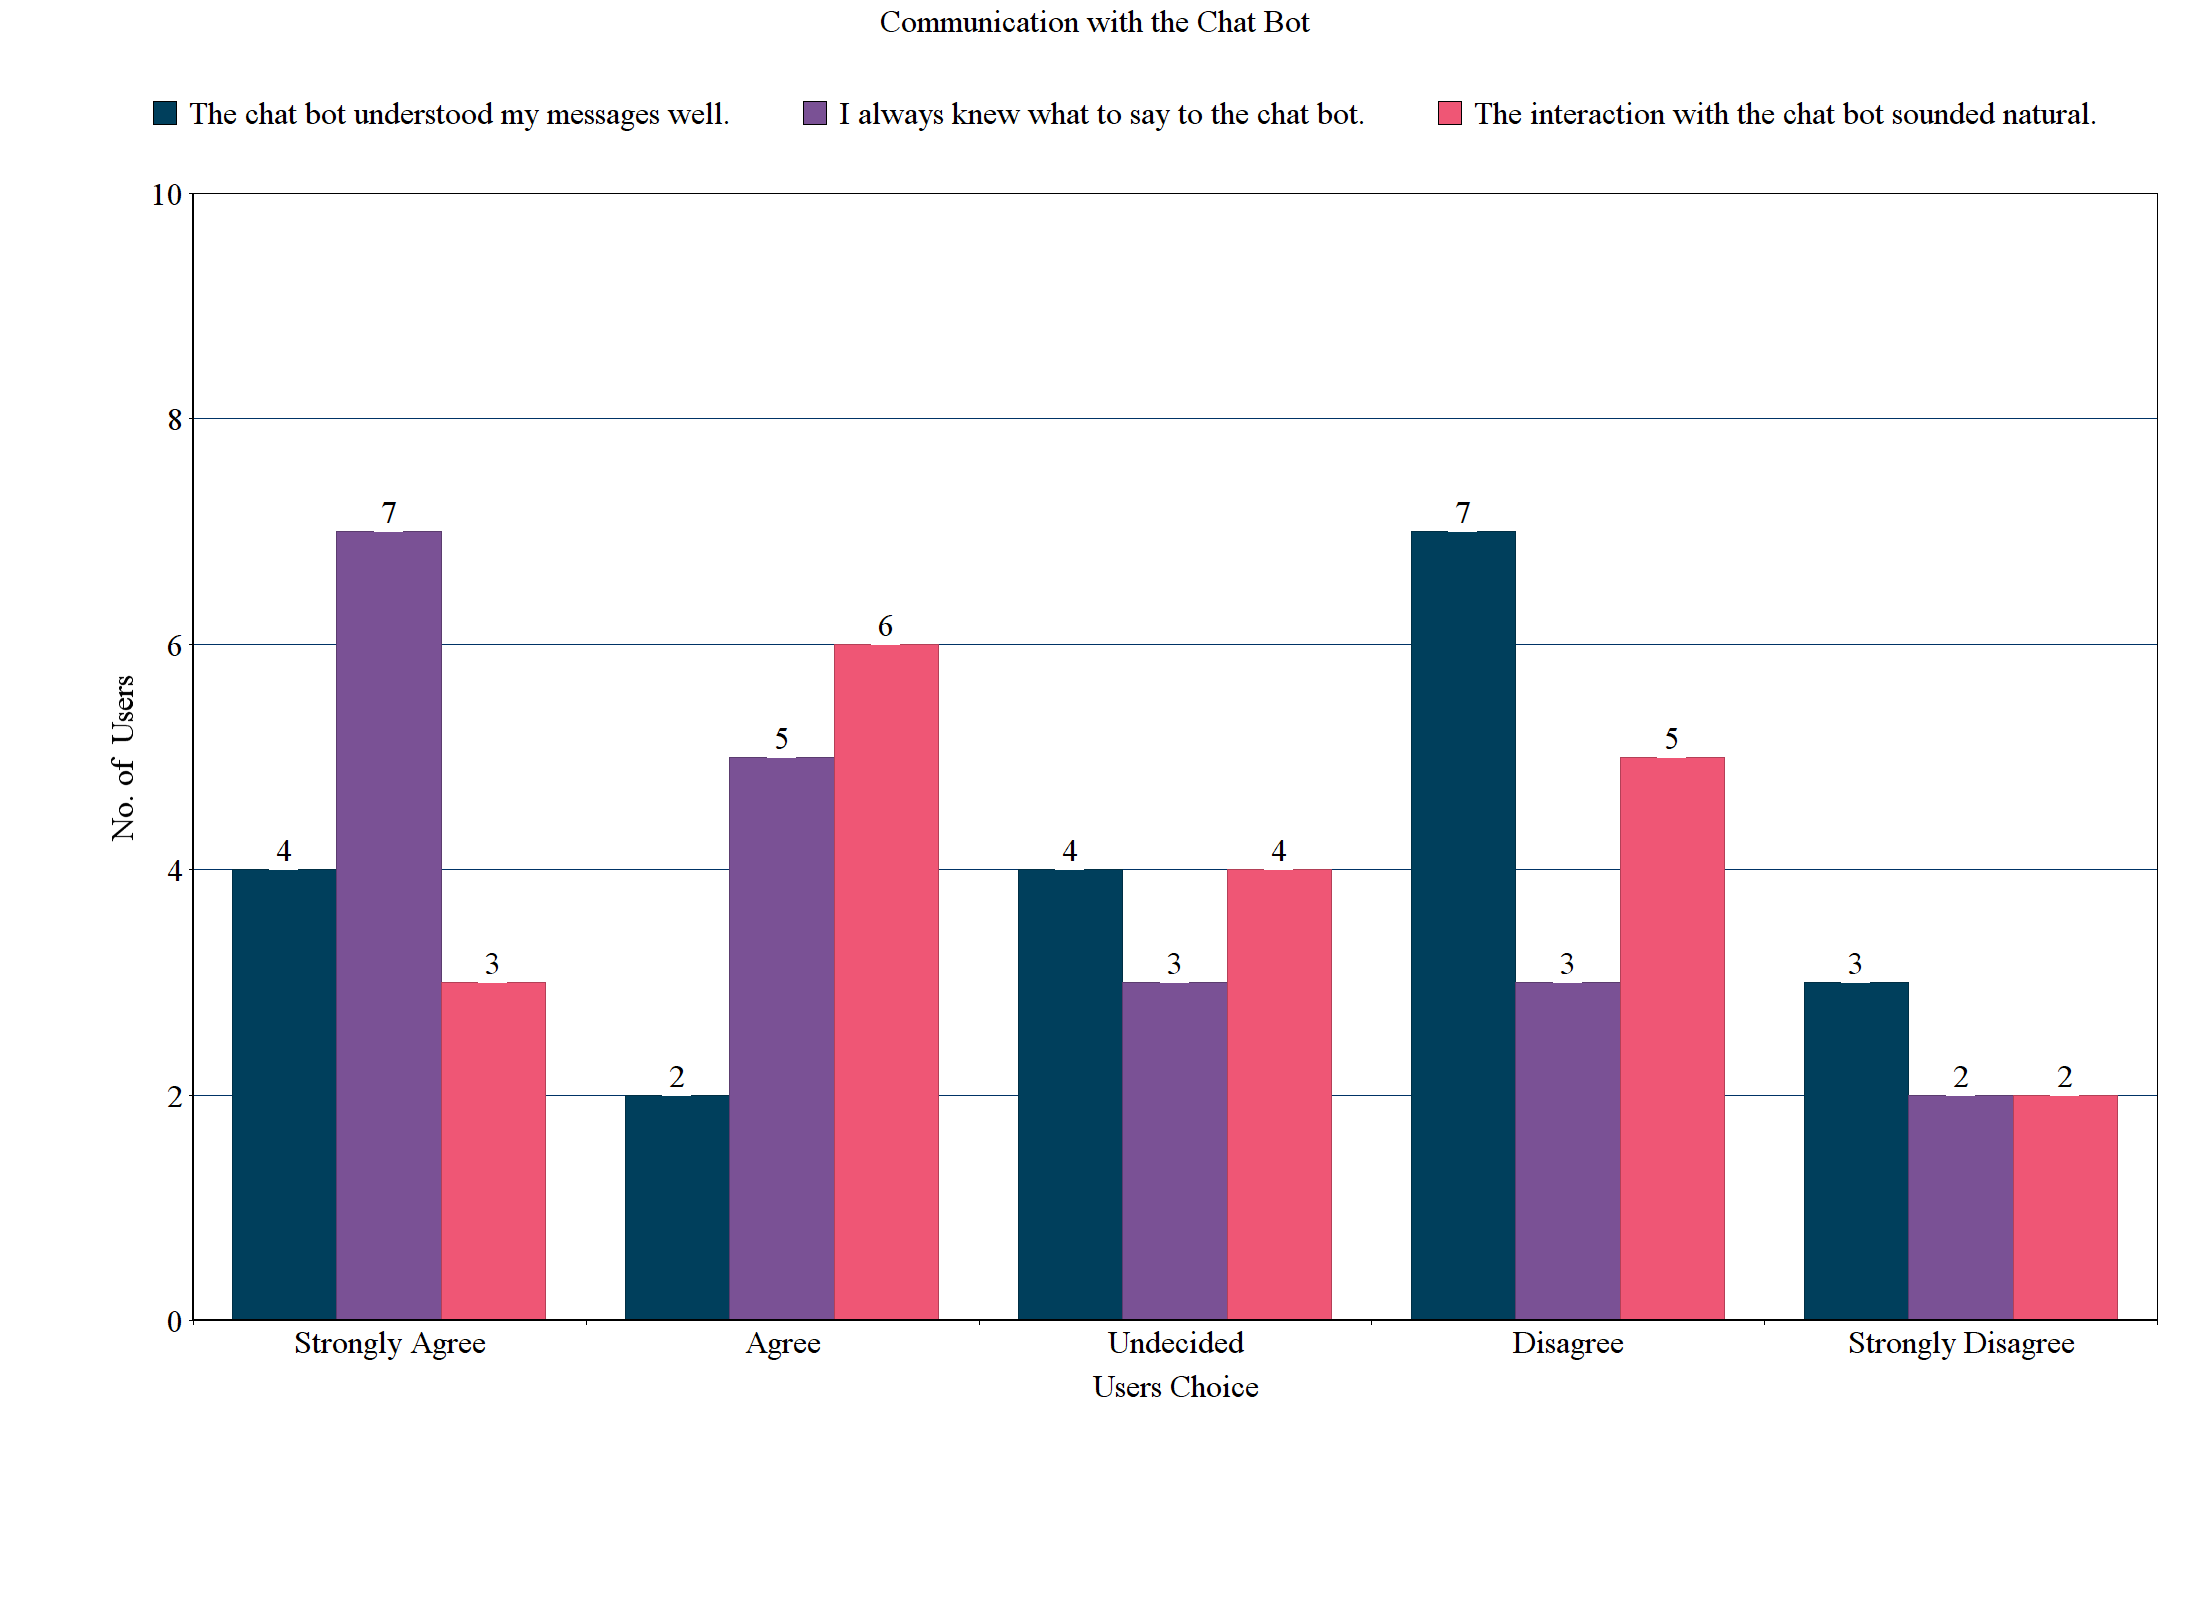
\includegraphics[width=0.9\textwidth]{img/Communication_with_the_Chat_Bot_Updated.png}
    \caption{Graphical representation of results collected for the users communication with the chat bot.}
    \label{fig:communwithBot}
\end{figure}
\\~\\
As extracted from graphical representation in Figure \ref{fig:communwithBot} that the total 10(50\%) of the participants disagreed with the statement that the chatbot understood their messages well. And 4(20\%) out of the remaining 10 were not able to decide about it. Remaining 6(30\%) answered positively with it. As majority disagreed with the statement and a reason could be the chatbot responded incorrectly. And it could be due to a problem with natural language understanding. It has been observed while testing that NLU was detecting wrong intents for the inputted utterances. The possible justification for it could be the limited training data used for learning as already mentioned in Section \ref{sec:expchatbot}. And the intents used in training has been displayed in Appendix \ref{appen:traindatastats}.

% \begin{figure}[!h]
%     \centering
%     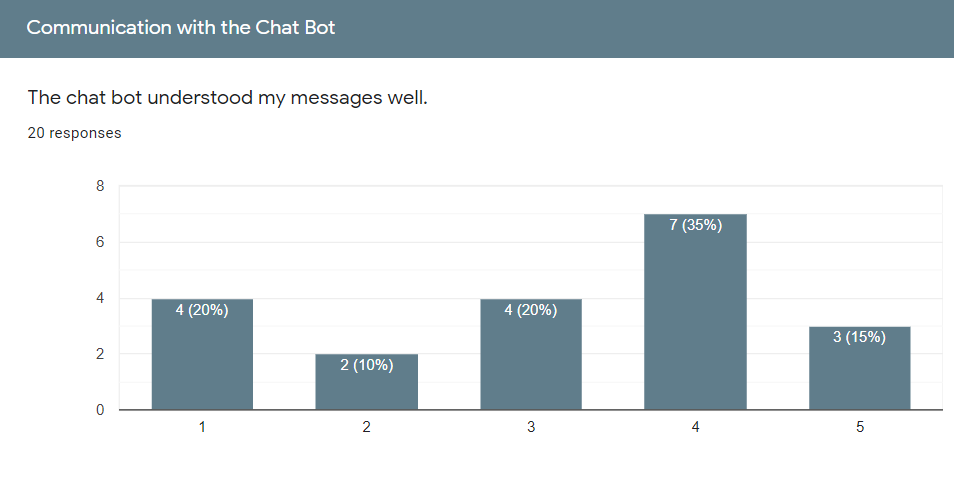
\includegraphics[width=0.9\textwidth]{img/Underst_Well.PNG}
%     \caption{Responses for the statement that the chat bot understood messages well.}
%     \label{fig:understWell}
% \end{figure}
\\~\\
Coming towards the next statement from the Figure \ref{fig:communwithBot}, 12(60\%) of the users agreed that they always knew what to reply or ask the chatbot. Other than those, 3(15\%) failed to make any decision about it and remaining 5(25\%) disagreed with it. 
% Results have been displayed in the Figure .
% \begin{figure}[!h]
%     \centering
%     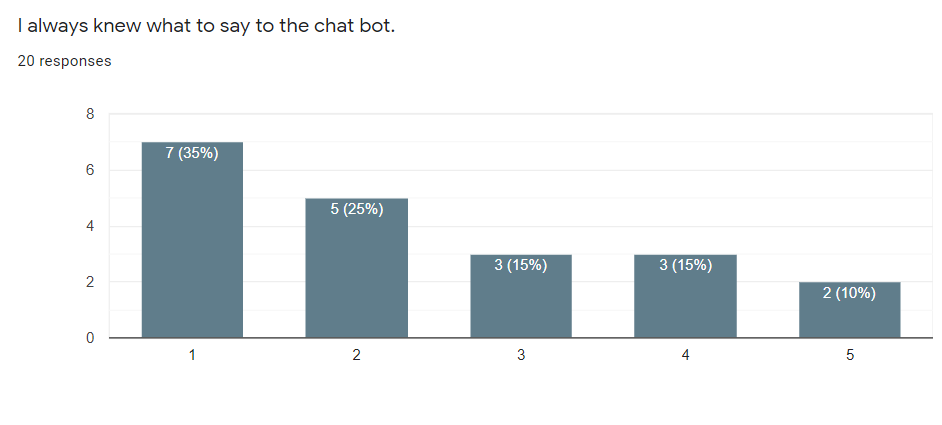
\includegraphics[width=0.9\textwidth]{img/Say_to_Bot.PNG}
%     \caption{Responses for the statement that the user always knew what to say to the chat bot.}
%     \label{fig:saytoBot}
% \end{figure}
\\~\\
Responses for the third statement from the Figure \ref{fig:communwithBot} showed that 9(45\%) participants felt the communication as natural. Out of other 11 only 4(20\%) failed to decide about it. Along with that remaining 7(35\%) showed disagreement with it. And the reason could be the wrong intent detection by NLU. It has been observed through the information collected using a log file. Secondly, manually fed responses could also be a reason for it as every time it has to select from fixed number of answers.
% For visuals, kindly have a look in to the Figure .
% \begin{figure}[!h]
%     \centering
%     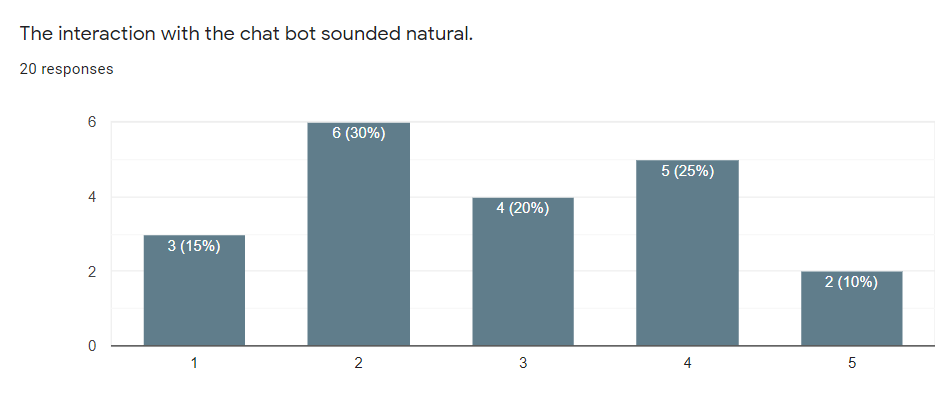
\includegraphics[width=0.9\textwidth]{img/Natural_Inter.PNG}
%     \caption{Responses for the statement that the interaction with the chat bot sounded natural.}
%     \label{fig:naturalInter}
% \end{figure}

\subsubsection*{Behaviour of the Chat Bot}
Intentions behind adding this section to the questionnaire was to detect the behaviour of the chatbot with the user. It consisted of the seven questions answered by the user on the scale of agreement or disagreement as stated below: 
\begin{enumerate}
    \item The chat bot responded too slowly.
    \item The chat bot is friendly.
    \item The chat bot didn't always meet my expectations.
    \item I didn't always know what answer the chat bot is expecting from me.
    \item The chat bot made many errors.
    \item I was able to recover easily from errors. (only in case of errors).
    \item The chat bot behaved in cooperative way.
\end{enumerate}
Graphical representation for the detailed analysis and comparison of the results for these statements has been shown in the Figure \ref{fig:behavofBot}.

\begin{figure}[!h]
    \centering
    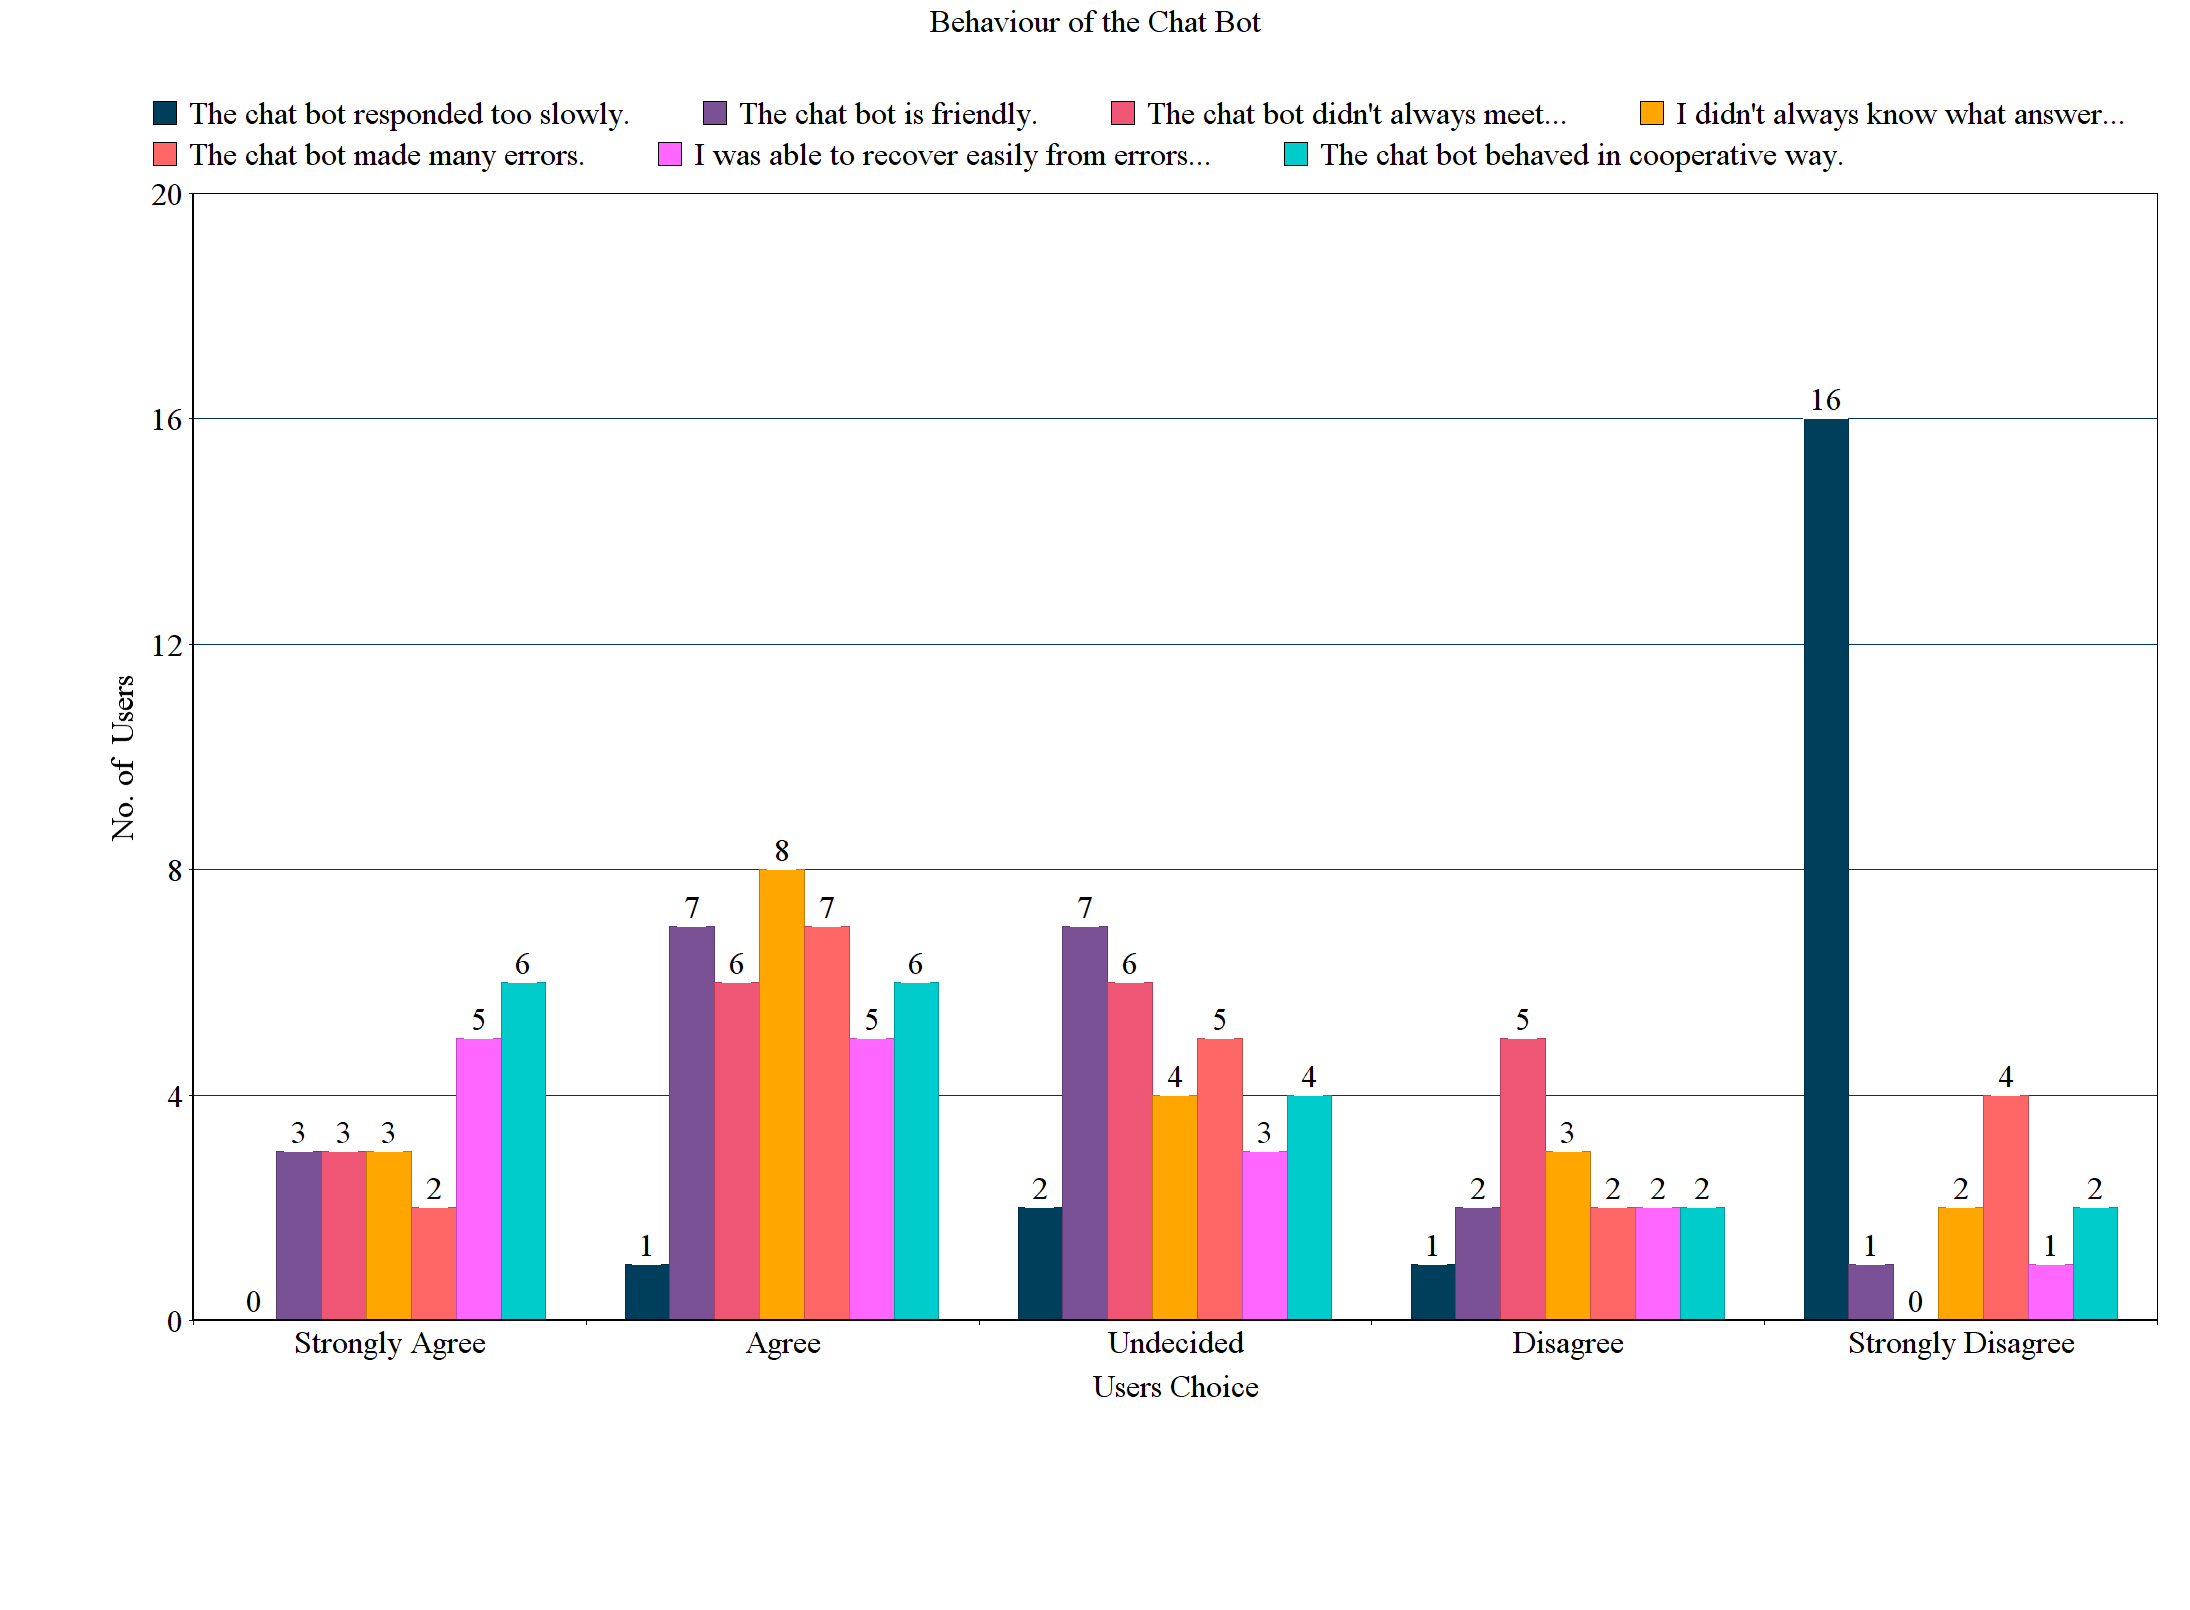
\includegraphics[width=0.9\textwidth]{img/Behaviour_of_the_Chat_Bot_Updated.png}
    \caption{Graphical representation of results collected for the behaviour of the chatbot.}
    \label{fig:behavofBot}
\end{figure}
\\~\\
Analysing the results for this section's initial statement, 16(80\%) strongly disagreed with it. Whereas, another 1(5\%) also negated the statement which makes the number total 17(85\%) who portrayed that the responding speed for the chatbot was fast enough as shown in the Figure \ref{fig:behavofBot}. 

% \begin{figure}[!h]
%     \centering
%     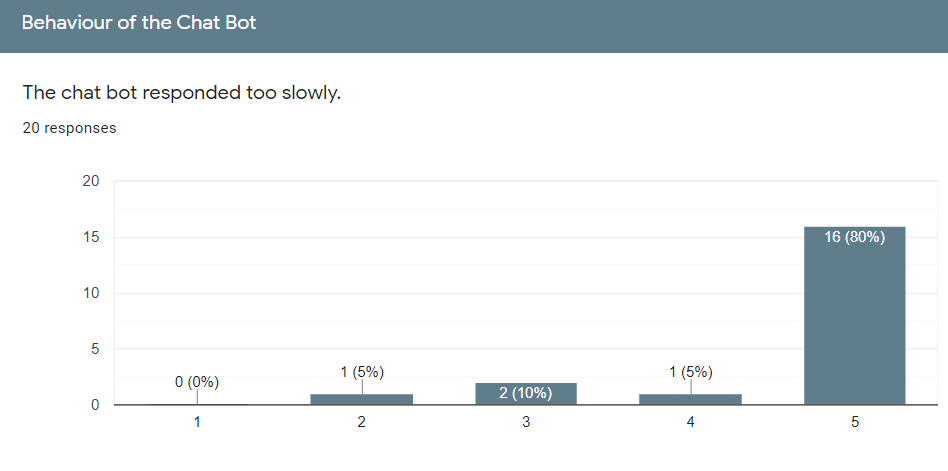
\includegraphics[width=0.9\textwidth]{img/Response_Speed.PNG}
%     \caption{Result about the chat bot's response speed}
%     \label{fig:respSpeed}
% \end{figure}
\\~\\
Secondly, 10(50\%) rated the chatbot as friendly. While 7(35\%) other respondents were unable to come up with any decision about it as displayed in the Figure \ref{fig:behavofBot}. It could be due to the reason that different persons have their own perception about friendliness. Also, the demo topic included the detective bot. So, it was meant to respond with straight forward statements. Which could be felt a bit offensive some times depending upon the user's mood and nature. 

% \begin{figure}[!h]
%     \centering
%     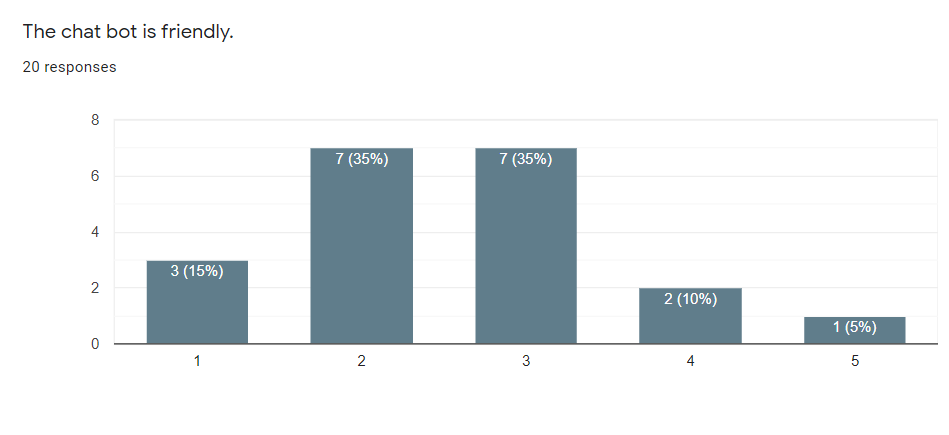
\includegraphics[width=0.9\textwidth]{img/Friendly_Chatbot.PNG}
%     \caption{Result about the chat bot's friendliness}
%     \label{fig:friendlyBot}
% \end{figure}
\\~\\
Thirdly, the chatbot didn't meet the expectations for 9(45\%) of the participants. Additionally, other 6(30\%) were failed to determine about it and only 5(25\%) stated that it fulfilled their expectations and can be visualized in the Figure \ref{fig:behavofBot}. So it can be clearly concluded from it that the chatbot failed to impress the users by its behaviour. The possible reason for it might be same to the statement in the last section that the chatbot didn't understand the messages well or the users found it harsh or offensive.

% \begin{figure}[!h]
%     \centering
%     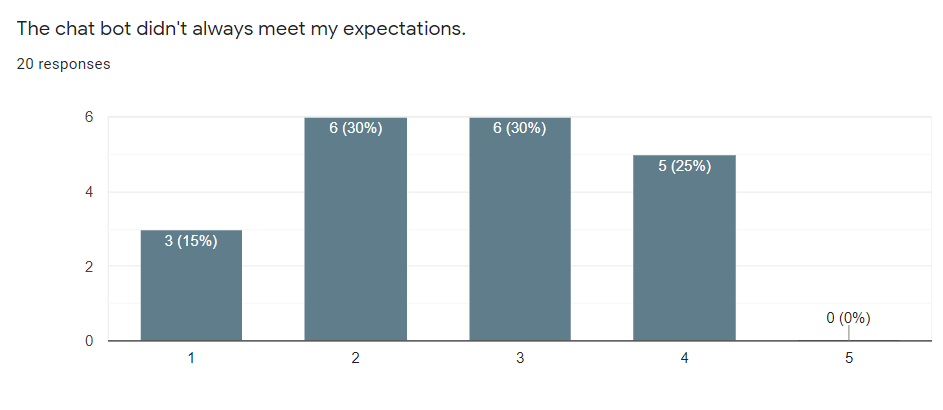
\includegraphics[width=0.9\textwidth]{img/Chatbot_Expect.PNG}
%     \caption{Result for the expectations from the chat bot}
%     \label{fig:botExpec}
% \end{figure}
\\~\\
Reviewing the results for the forth statement, 11(55\%) of the respondents showed agreement with the statement that they didn't always know what answer was the chatbot expecting from them as displayed in the Figure \ref{fig:behavofBot}. It could be due to the limitation of the training data as the chatbot was just trained for limited intents but the users were provided with free choice to ask anything from the chatbot. 

% \begin{figure}[!h]
%     \centering
%     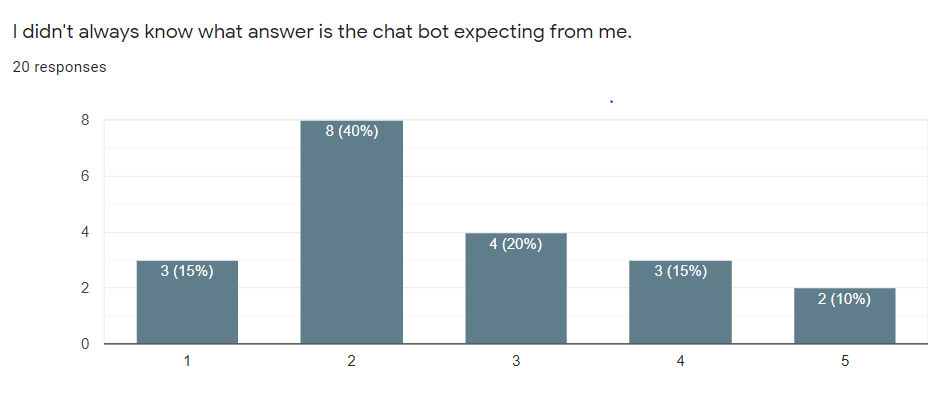
\includegraphics[width=0.9\textwidth]{img/Answer_Expect.PNG}
%     \caption{Result for the users knowledge about the chatbot's expectation}
%     \label{fig:ansExpec}
% \end{figure}
\\~\\
Checking with the participants opinion about errors made by the chatbot and recovery from them, 9(45\%) stated that chatbot made errors. While 6(30\%) negated it and remaining 5(25\%) were unable to decide about it. But the positive point about the chatbot was, out of those users who faced the error or unable to decide about it during a chat, 10 of them were able to recover easily from the error. In addition to that, 12(60\%) of the participants rated the chatbot as cooperative. On contrary, just 4(20\%) marked it as uncooperative as shown in the Figure \ref{fig:behavofBot}.

% \begin{figure}[!h]
%     \centering
%     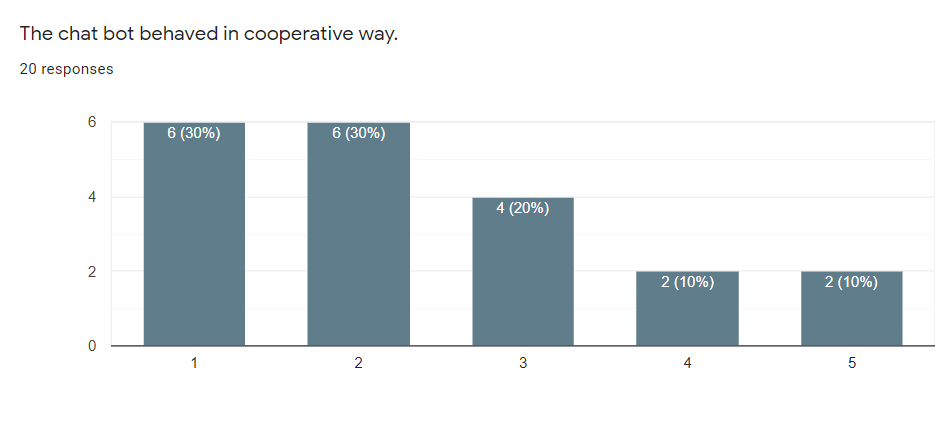
\includegraphics[width=0.9\textwidth]{img/Cooperative_Chatbot.PNG}
%     \caption{Result about the the chatbot's cooperativity}
%     \label{fig:cooperBot}
% \end{figure}

\subsubsection*{Dialogue Assessment}
This part of the survey was added to judge the design of the dialogue according to the users perspective. Total six question were asked by the participants for completion of the purpose.
\begin{enumerate}
    \item I easily lost track of where I am in an interaction with the chat bot.
    \item The dialogue was bumpy.
    \item I was able to direct the conversation as desired.
    \item I felt in control of the interaction with the chat bot.
    \item The dialogue quickly led to the desired goal.
    \item The dialogue parts were evenly distributed between me and the chat bot.
\end{enumerate}
Graphical representation for the detailed analysis and comparison of the results for these questions has been displayed in the Figure \ref{fig:dialogAssess}.

\begin{figure}[!h]
    \centering
    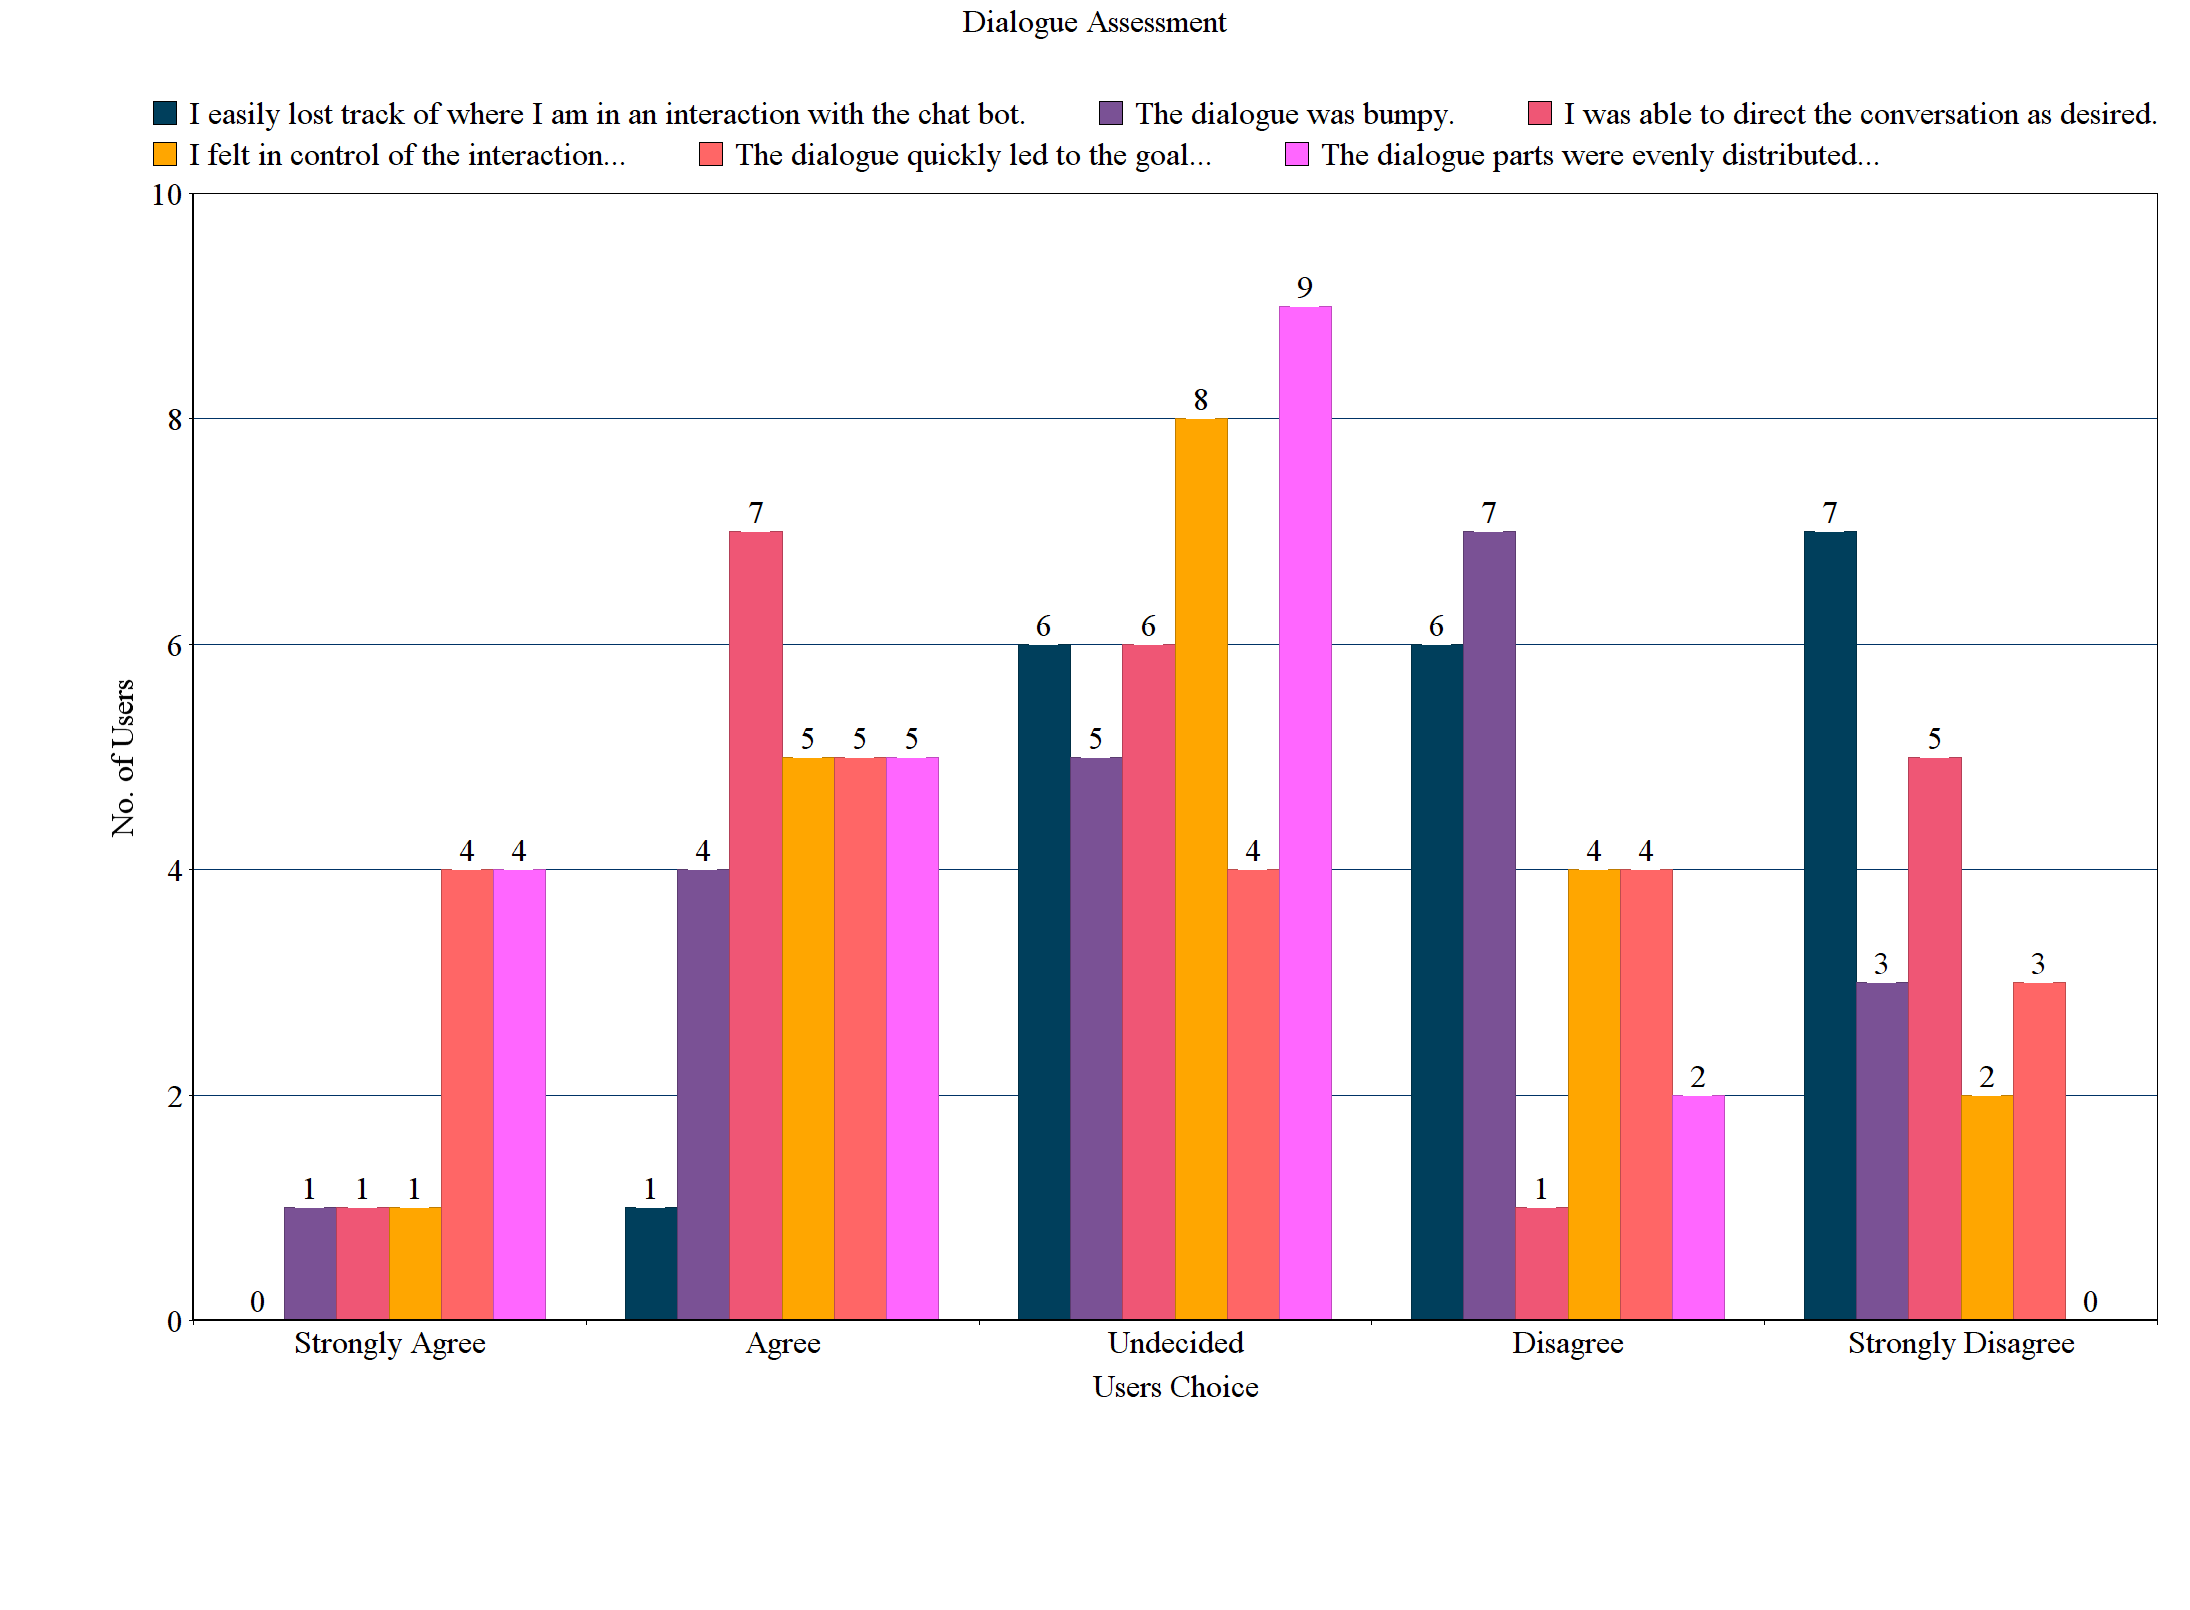
\includegraphics[width=0.9\textwidth]{img/Dialogue_Assessment_Updated.png}
    \caption{Graphical representation of results collected for the dialogue assessment.}
    \label{fig:dialogAssess}
\end{figure}
\\~\\
As plotted in the Figure \ref{fig:dialogAssess} that 7(35\%) strongly disagreed while 6(30\%) simply disagreed with the statement that they lost the track during the communication with the chatbot. On the other hand, 6(30\%) were unable to make any decision and only 1(5\%) just agreed with it. So it can be concluded from the result analysis that maintaining a state for each module with respect to each user has been appeared really useful and effective.

% \begin{figure}[!h]
%     \centering
%     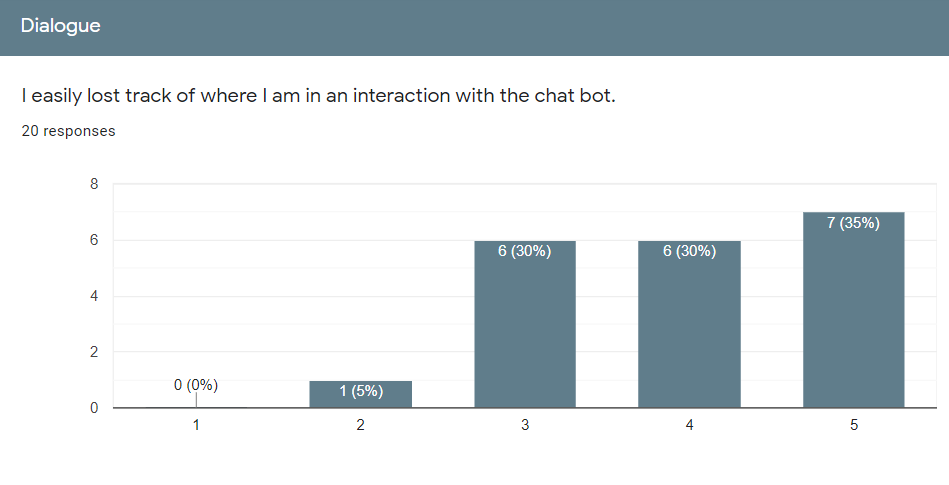
\includegraphics[width=0.9\textwidth]{img/Lost_Track.PNG}
%     \caption{Result for users lost track during interaction with the chatbot}
%     \label{fig:lostTrack}
% \end{figure}
\\~\\
After analysing the results from the Figure \ref{fig:dialogAssess}, it is not wrong to say that the dialogue was smooth and communication between the users and the chatbot was comfortable and consistent. As, 10(50\%) of the participants showed disagreement with the statement that the dialogue was bumpy. Contrarily, only half of it that is 5(25\%) just find it unstable. Which means by using the modular architecture a stable and smooth dialogue can be designed.

% \begin{figure}[!h]
%     \centering
%     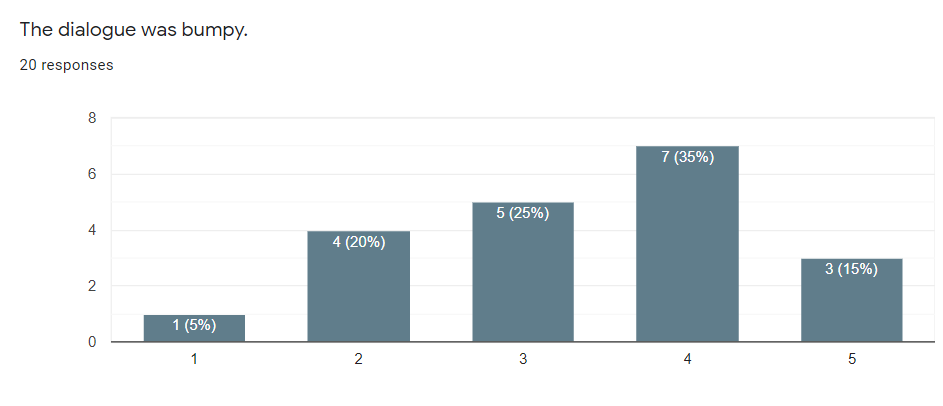
\includegraphics[width=0.9\textwidth]{img/Bumpy_Dialog.PNG}
%     \caption{Result reflecting users opinion about bumpy dialogue}
%     \label{fig:bumpDialo}
% \end{figure}
\\~\\
Nextly, as presented in the Figure \ref{fig:dialogAssess} that 8(40\%) of the participants were able to direct the conversation according to their desires. On the other hand, 6(30\%) out of the remaining 12 were unable to drive it according to their wish. And the left out 6(30\%) answered as undecided. And yet again the ratio of the respondents who were able to direct the conversation as desired appeared to be greater than the ones who were not be able to do it.

% \begin{figure}[!h]
%     \centering
%     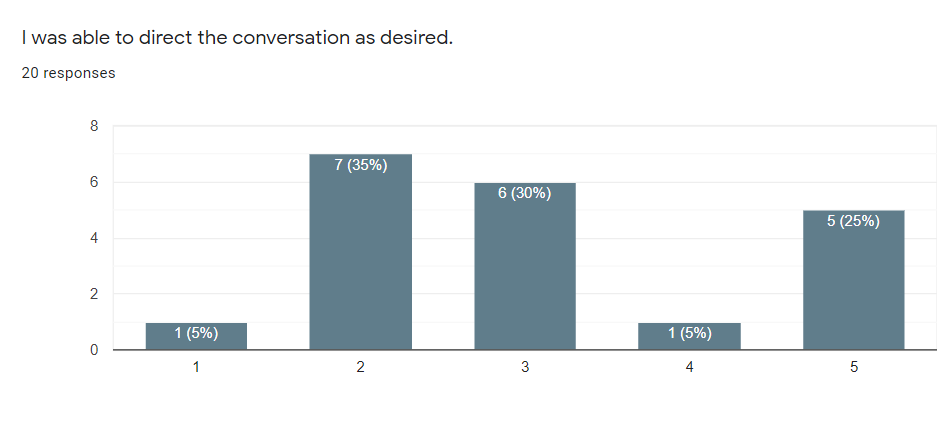
\includegraphics[width=0.9\textwidth]{img/Desired_Conv.PNG}
%     \caption{Result reflecting users opinion about desired conversation}
%     \label{fig:desiredConv}
% \end{figure}
\\~\\
As shown in the Figure \ref{fig:dialogAssess}, that the number of participants who agreed and disagreed with the statement that they felt in control of the conversation with the chatbot is same and that is 6(30\%) for both categories. And remaining 8(40\%) were not able to decide about it. Now it is something alarming, as in this case a possible reason could be the topic of the demo chatbot. As I designed the detective chatbot and it was designed in a way to be a bit strict and commanding. 

% \begin{figure}[!h]
%     \centering
%     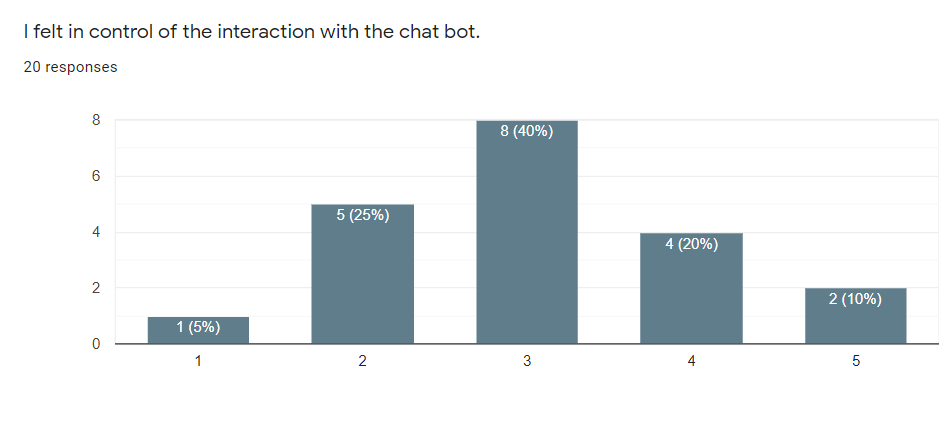
\includegraphics[width=0.9\textwidth]{img/Chatbot_Control.PNG}
%     \caption{Result reflecting users opinion whether they felt that the chat was controlled by the chatbot}
%     \label{fig:chatbotControl}
% \end{figure}
\\~\\
According to the Figure \ref{fig:dialogAssess}, 9(45\%) answered that the dialogue quickly led to the desired goal which refers to the fact that the detective game was designed in such manner that the user should be able to reach the final goal as quickly as possible. But also 7(35\%) disagreed with it and the cause behind it could be the wrong intent detection as user typed in something else but NLU recognized it differently due to which chatbot responded with some unrelated statement.

% \begin{figure}[!h]
%     \centering
%     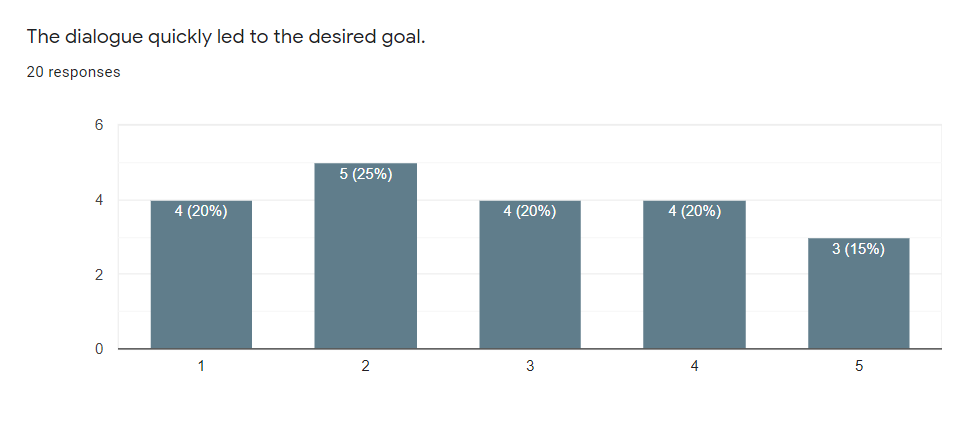
\includegraphics[width=0.9\textwidth]{img/Quick_Goal.PNG}
%     \caption{Result reflecting users opinion about the dialogue quickly led to the goal}
%     \label{fig:quickGoal}
% \end{figure}
\\~\\
Referring to the Figure \ref{fig:dialogAssess}, 9(45\%) of the people who took part in the study agreed with a statement that dialogue parts were equally distributed between them and chatbot. Whereas, other 9(45\%) were leave it undecided and only 2(10\%) disagreed with it.

% \begin{figure}[!h]
%     \centering
%     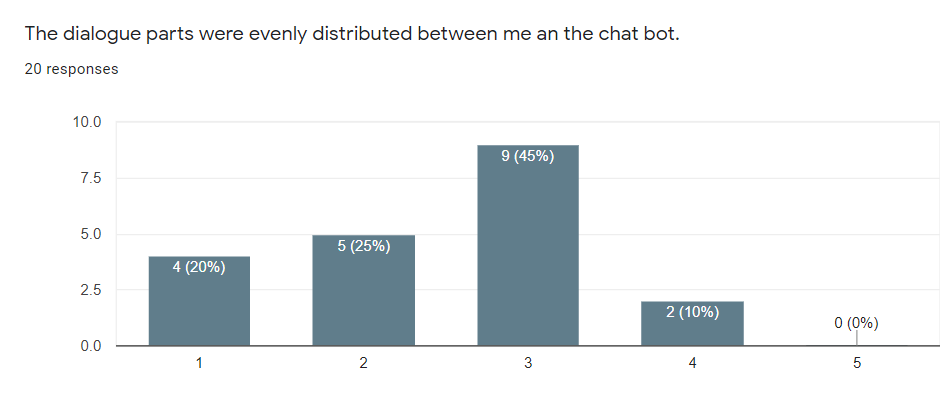
\includegraphics[width=0.9\textwidth]{img/Even_Parts.PNG}
%     \caption{Result reflecting users opinion about the equal distribution of the dialogue parts}
%     \label{fig:evenDist}
% \end{figure}

\subsubsection*{Personal Experience and Impression}
This segment has been put to the questionnaire in order to collect users experience and personal impression about the chatbot. It also has been completed using series of questions. 
\begin{enumerate}
    \item The interaction with the chat bot was pleasant.
    \item I felt relaxed.
    \item High level of concentration is required while using the chat bot.
    \item The interaction was fun.
    \item Overall, I am satisfied with the chat bot.
    \item I felt that the chat bot was smart enough to handle the message which was not lying in its scope.
    \item I felt that the chat bot guided me well to return to the actual topic when I tried to misguide it.
    \item It was easy for me to continue the chat without any reluctance.
    \item It was easy for me to understand the response of the chat bot.
    \item It took me too long to make the chat bot understand my message by using different terms in sentences.
\end{enumerate}
Graphical representation for the detailed analysis and comparison of the remarks for these assertions has been shown in the Figure \ref{fig:persExpandImp}.

\begin{figure}[!h]
    \centering
    \includegraphics[width=0.9\textwidth]{img/Personal_Experience_and_Impression_Updated.png}
    \caption{Graphical representation of results collected for the users personal experience and impression.}
    \label{fig:persExpandImp}
\end{figure}
\\~\\
As presented in the Figure \ref{fig:persExpandImp}, majority of the participants i.e. 12(60\%) felt that the interaction with the chatbot was pleasant. It could be due to the reason that the user doesn't have to restart the chat whenever he/she wants to move to some different topic. The user was able to jump between different topics at any moment and can handle multiple topics at the same time without loosing the state for the last topic. 
\\~\\
According to the Figure \ref{fig:persExpandImp}, 11(55\%) respondents responded that they felt relaxed while having a conversation with the chatbot. It was something important to make sure that chatbot is not making someone feel tensed or bad about anything. Furthermore, 10(50\%) of the users also showed disagreement to the statement that high level of concentration was required while using the chatbot. So, from this result it can be concluded that the chatbot and the dialogue design was simple and also user friendly. Additionally, 15(75\%) of the users found the interaction as fun. It was also the main purpose of the Frankenbot to entertain the users instead of making them feel bored. So, this purpose also gets accomplished. 
\\~\\
After analysing the result from the Figure \ref{fig:persExpandImp} about the user satisfaction for the chatbot, it can be deduced that the majority of the users 10(50\%) felt satisfied with it. While, 5(25\%) out of the other 10 left it undecided and the remaining 5(25\%) were not satisfied with it.
\\~\\
Nextly, as figured out from the Figure \ref{fig:persExpandImp}, majority 8(40\%) of the participants disagreed that the chatbot was able to handle the messages well which were out of its scope. Whereas, 7(35\%) of the respondents agreed with it. By surveillance of the log file on the basis of detected intents for user utterances, it has been observed that the wrongly recognized intent could be a reason for it. Otherwise, framework has been tested in such a way that, if on each step an utterance is provided from training data and intent has been identified correctly then its performance was up to the mark. Secondly, it has been designed to handle such scenario well as already explained in the Chapter \ref{cha:chapter3} of this document. In addition to it, 14(70\%) of the respondents showed agreement to the statement that chatbot guided them well to return to the actual topic when they tried to misguide it. It makes the stance clear about the chatbot abilities that it contains the skills to well manage the messages which do not lie under its scope.
\\~\\
Moving to the next statement, 10(50\%) of the users agreed that they were able to continue the chat without any stoppage. It means the chatbot was working well for them as they wanted. The chatbot nor the user were reluctant to each other. It can also be concluded from this result that the dialogue was well structured and designed in order to perform smooth conversation without any objection or hesitation. Another important factor that can't be neglected is that the user should be able to understand the chatbot's response. So, 13(65\%) of the participants were able to do so. Which also marked this property as accomplished for the chatbot.
\\~\\
Lastly, 12(60\%) out of the total 20 participants negated the statement that it took them too long to make the chat bot understand their message by using different terms in sentences. It reflects that the information provided to the users was pretty much clear and also the guidance by the chatbot was enough for the user to enter correct answer.

\subsubsection*{Usability}
This part of the survey has been added to gather the users opinion about the chatbot's usefulness and whether it is easy to use or not. So, it has been judged on the basis of what users have answered to the following questions:
\begin{enumerate}
    \item The system is difficult to use.
    \item It is easy to learn to use the chat bot.
    \item The chat bot is too inflexible.
    \item I would like to use the chat bot again in the future.
    \item The chat bot operation was worthwhile.
\end{enumerate}
Graphical representation for the detailed analysis and comparison of the responses for these assertions has been shown in the Figure \ref{fig:usabil}.

\begin{figure}[!h]
    \centering
    \includegraphics[width=0.9\textwidth]{img/Usability_Updated.png}
    \caption{Graphical representation of results collected for the chatbot's usability.}
    \label{fig:usabil}
\end{figure}
\\~\\
According to the result deduced from the Figure \ref{fig:usabil}, 15(75\%) of the users contradicted with the statement that the chatbot was difficult to use. Which means the majority of the participants found it easy to use. Additionally, again the same amount of the respondents i.e. 15(75\%) discovered that it was easier to understand the chatbot. It could be due to several reasons like the information provided was enough, the chatbot's ability to guide the user, structured dialogue and good understanding of the chatbot's response by the user.
\\~\\
Furthermore, 8(40\%) of the respondents disagreed with the statement that chatbot was too inflexible. Whereas, 7(35\%) showed agreement on this statement. This mixed opinion of user could be just because of the reason that the chatbot was designed in a way that it should guide the user to return to the actual topic instead of continuing the chat on any user's desired topic. As the chatbot has been trained using limited data, time and resources. Once, it will undergo good training then one can easily make it work for all user utterances regardless of the specific topic.
\\~\\
At the end, the users were asked whether they want to use the chatbot again in future. And 11(55\%) replied positively. Contrarily, only 4(20\%) responded negatively. Moreover, they were also asked to rate the chatbot's functioning whether it's worth the time and effort spent. And majority i.e. 11(55\%) of the participants agreed with it. On the other hand, only 4(20\%) of respondents disagreed with it.

\subsection{Evaluation via AttrakDiff}
AttrakDiff's single evaluation method\footnote{\url{http://www.attrakdiff.de/#tab-einsatz}} has been used in order to judge the chatbot on the basis of the following qualities:
\begin{itemize}
    \item Hedonic quality (HQ), it includes 14 word pairs which refers to the joy of use, emphasized stimulation, identification and evocation generated by the system.
    \item Pragmatic quality (PQ), it involves 7 word pairs which reflect the system's usefulness, efficiency and how easy is it to use.
    \item Attractiveness (ATT), it is also comprised of 7 items that are being used to judge the system's pleasantness and how catchy is it according to the user's point of view.
\end{itemize} 

\subsubsection*{Word Pairs}
Coming to the results gathered using Attakdiff's questionnaire and also what word pairs have been used in single evaluation method along with the mean of ratings by participants and standard deviation have been displayed in the Figure \ref{fig:descofWordPair}.

\begin{figure}[!h]
    \centering
    \includegraphics[width=1\textwidth]{img/Desc_of_Word_Pairs.png}
    \caption{Description of the word pairs along with the mean values and standard deviation \cite{attrakdiff}.}
    \label{fig:descofWordPair}
\end{figure}
\\~\\
The AttrakDiff questionnaire contains the information for pragmatic and hedonic quality of an interactive system. The language of the study was English but the participants also had an option for German.
\\~\\
As shown in the Figure \ref{fig:descofWordPair}, the linear scale has been appointed the values from -3 to +3. The values -3 to -1 has been assigned to the negative aspect of the word pair e.g. "unpleasant". While, 0 lies in middle of the negative and positive aspects and referred as neutral. Whereas, the range from +1 to +3 has been referred to the positive aspect of the word pair e.g. "pleasant".
\\~\\
The division of the word pairs according to their groups and classification with seven items each can also be inferred from the Figure \ref{fig:descofWordPair}. The word pairs starting from "technical - human" till "unruly -manageable" lies under the pragmatic (PQ) category. Furthermore, word pairs from "isolating - connective" to "unpresentable - presentable" falls under hedonic attribute group named Identification (HQ-I). Additionally, word pairs ranged from "conventional - inventive" and till "ordinary - novel" have been put under the shadow of hedonic stimulation (HQ-S). Lastly, Attractiveness (ATT) includes the set of the word pairs starting from "unpleasant - pleasant" and ending on "discouraging - motivating". 
\\~\\
Overall, the pragmatic quality for the chatbot rated by the participants is positive. It has been deduced from the results displayed in the Figure \ref{fig:descofWordPair}. Respondents rated it neither technical nor human. The initial goal is achieved that at least the users didn't find it task-oriented or following some order. It is the first step towards more humanly. On the other hand, they are unable to discover its humanly characteristics. The possible reason for it could be lack of ability to generate a natural responses on the basis of real communication. As it has been stuffed manually with fixed number of responses. Moreover, the inadequate amount of data containing limited number of intents (shown in Appendix \ref{appen:traindatastats}) has been used for training purpose. It could also be a reason for such feedback. Secondly, users rated it "Simple" with the positive mark greater than 1. The greatest peak at the positive side for the pragmatic section goes near to 2 for the term "Straightforward". Which means it was easy to understand and was uncomplicated. Moreover, users also found the chatbot practical, clearly structured, and manageable. The only negative point almost near to 0 has been encountered i.e. the chatbot is unpredictable. The possible reason for it could be the responses of the demo detective bot. But it has been designed like this for fun purpose. So by the results it has been inferred that the users found the chatbot useful and assisting in order to achieve the desired goal.
\\~\\
Moving to the hedonic assessment, firstly hedonic identification ability (HQ-I) of the system has been tested using different word pairs that how the chatbot is delivering the important personal values. It can also be inferred from the results portrayed in the Figure \ref{fig:descofWordPair} that as a whole HQ-I appeared to be positive. The participants of this study graded the chatbot as connective, professional, stylish, integrating, and highly presentable. As the word pair "cheap - premium" is answered as neutral and it could be because of the shortness, unreality and immaturity of a dialogue due to the limitations of training data and responses. The positivity deduced from it is at least a chatbot is not ranked low in quality. Contrarily, neither it is rated as prime featured may be due to the definite dialogue topics or absence of any real time achievement. Furthermore, ranking for "separates me - brings me closer" highlights that neither the majority felt isolated or get apart with it nor they get attracted to it. It raised a need of improvement to make it more delivering and catchy for the users. It can be inferred from overall analysis that the chatbot accomplished its task to deliver the values that users were expecting from it and fulfilled the users expectations. But still there exist some areas that must be subjected to improvements.
\\~\\
Moreover, hedonic stimulation (HQ-S) has been used to measure the chatbot's challenging ability according to the users perspective. Overall results for it have shown positive trend. The users found it inventive, highly creative, bold, innovative, captivating and challenging. But the arc for the term "ordinary - novel" has been graded as neutral. As users can see many other much improvised and state of the art chatbots like Google's Assistant, Apple's Siri and Amazon's Alexa. So, they just considered it as a normal chatbot. It could be the reason that they neither rated it as ordinary nor novel. But instead of that by taking overall result in to an account, the users found it challenging, interesting and fascinating.
\\~\\
Finally, attractiveness has been measured for the chatbot by taking the results from PQ and HQ in to the consideration and by using separate related word pairs for it. By the results gathered from the participants responses, it can be stated undoubtedly that all the users found it pleasant and attractive as the values for all the terms are positive. Which also makes it likeable, inviting, good, appealing and motivating.

\subsubsection*{Average Values}
According to the Figure \ref{fig:avgValAttrak}, if the average values are considered to grade the quality of the chatbot then it is not wrong to say that the attractiveness(ATT) has the highest value 0.75 and standard deviation(SD) of 0.15. While, pragmatic quality(PQ) has been placed at second position with the mean value of 0.72 and SD of 0.67. On the other hand for hedonic quality's race, the challenging aspect of the chatbot is leading as hedonic stimulation(HQ-S) has the mean value 0.56 with SD as 0.34. Moreover, the chatbot succeeded in delivering the important values to the users at the lowest with an average of 0.46 and SD as 0.35. As it is not wrong to say that the initial chatbot has been rated well in all aspects. But the average values lie just under the category of lower positive. None of the sections collectively crossed the mark of +1 whereas the maximum limit that can be reached is +3. So, as the initial start these results can be considered as good. But it will not be lame to say that the chatbot must go through some more training, structuring and designing in order to get improved in its next version to reach the desired level for its users.

\begin{figure}[!h]
    \centering
    \includegraphics[width=0.8\textwidth]{img/Diagram_for_Avg_Values.png}
    \caption{Average values for PQ, HQ-I, HQ-S and ATT \cite{attrakdiff}.}
    \label{fig:avgValAttrak}
\end{figure}

\subsubsection*{Portfolio Discussion}
The dimensions for the portfolio of hedonic and pragmatic qualities have been displayed in the Figure \ref{fig:portRes}. The vertical axis represents HQ(bottom = low value) while horizontal axis depicts PQ(left = low value). In the portfolio presentation, the outer bigger light blue rectangle is the confidence rectangle. It shows that how divergent are the users in evaluating the product. The bigger is the confidence rectangle, more diverged and less confident are the gathered results. The small dark blue spot is representing the actual rating of the system. The actual value for the PQ is 0.72 and HQ is 0.51. It can be visualized that the chatbot falls in to the upper neutral area for both of the dimensions (PQ and HQ). Whereas, the confidence rectangle calculated by the users agreement shows that the confidence interval for PQ is dispersed between neutral and task-oriented character-regions. Whereas, for HQ it falls below the self-oriented region. It illustrates that there is a room for optimization in both dimensions but more likely for HQ as compared to PQ. If the hedonic quality could be raised by optimizing the natural language understanding for the chatbot using enriched and sufficient training data. Then user can communicate with it in a much better way and chatbot can also be able to deliver its best and users could find it more joyful and delivering. Although, pragmatically it is touching the task-oriented area for now but still needs to be elevated by improving the provided assistance for the users to achieve their desired goals. By undergoing such enhancements it can reach the region of desired characteristics.

\begin{figure}[!h]
    \centering
    \includegraphics[width=0.7\textwidth]{img/Portfolio_of_results.png}
    \caption{Portfolio of the results for HQ and PQ of the chatbot \cite{attrakdiff}.}
    \label{fig:portRes}
\end{figure}

\section{Qualitative Analysis}
This section illustrates the incidents and behaviours that have been observed during the accomplishment of this research study. Some of the following characteristics have been noticed and reported in a verbal interview conducted by consulting 12 actors out of total 20 participants.

\subsection{Natural Language Understanding(NLU)}
It has been examined while performing self testing on it that when the chatbot was inputted with the longer utterances, it was not able to identify the correct intent. Also whenever it has been asked for something that it is not trained for, the NLU was detecting the wrong intent. It is a real problem that could be a cause of confusion for the users and could also have made them to lose their interest.
\\~\\
Out of total 12, 8 of the interviewed participants started the interaction with greeting message and it worked well as the chatbot was designed so. But remaining 4 tried to start the communication with any other statement and they reported that the chatbot was smart enough to guide them that how to start the conversation. All of them revealed that once the dialogue has been initiated they tried to enter longer utterances but overtime shortened their sentences due to irrelevant responses. And with shorter and simple utterances the chatbot produced relevant answers. The possible reason behind it is the NLU training using limited data.
\\~\\
10 out of total 12 interrogated users changed terms in a sentence in order to make the chatbot understand the correct semantics of their statements. But at the end all of them were able to continue with the chat.

\subsection{Chatbot Guidance and Intelligence}
Also, 8 users reported that they were unable to move to the next question while playing a detective game but chatbot guided them well in order to make them understand what sort of input was it expecting from them at that specific moment. So, it can be deduced from it that the chatbot's ability to guide the user was good enough about the stuff for what it has not been trained or not expecting at some specific occasion. It was also able to deliver and to make the users to understand its responses well. Furthermore, 7 of the users notified that they tried to deviate the chatbot from the topic but the detective didn't get diverged and forced them using convincing responses to put them back on track.

\subsection{Interaction}
Total 12 participants were asked for the feedback about their interaction with the chatbot. And 11 of them replied that it was fun and they enjoyed the communication with chatbot. They also answered that the jokes it was cracking were really joyful and made them laugh. Other than that they also liked the sarcasm and strictness in the responses of the detective bot as it was designed for making users to feel that they are talking to some real detective. Only 1 out of 12 mentioned that the chatbot's answers were rude to some extent but when he was provided the reason for it then he realised and understood it. Conclusively, all the users who have been asked about the dialogue and the interaction with the chatbot, loved it.

\subsection{Switching Topics}
As it was mentioned in the description of the chatbot to the users that the chatbot has the ability to talk about parallel topics at the same time. The users have to switch the topic and come back to the previous topic by answering the last question of that topic at any moment in future. When the users have been asked about it in verbal conversation, all(12) of them mentioned that it worked fine and they really liked and appreciated this feature.

\subsection{Detective Game}
Same 12 participants have also been questioned to gather the feedback about detective game whether they liked it or not. To be precised, 6 out of them liked it and other 4 complaint about the short length of the game and the scenario was not directed well. In addition to it, remaining 2 found it as a source of recreation for them. Cumulatively, all of them liked the idea of the detective game as a demo. Also the users have been requested to end the game before moving to the completion of the surveys. And all of them replied positively on asking whether they reached an end of the game before filling out the questionnaires.

\subsection{User Interface}
9 out of the total 12 participants really liked the interface. But remaining 3 of them disliked it due to the dark theme as they recommended light coloured scheme for it. Otherwise, all of the users liked the design and style of an interface.  



    \chapter{Discussion and Conclusion\label{cha:chapter5}}
This is the final chapter for this master's thesis which summarizes it. Additionally, it also discusses the limitations of the framework stated in Chapter \ref{cha:chapter3} and evaluation methodologies along with the gathered results illustrated in Chapter \ref{cha:chapter4}. Lastly, possible future work has been manifested.

\section{Summary}
The motivation of this master's thesis was to implement a framework to enhance the development of conversational interfaces using a novel modular architecture discussed in Chapter \ref{cha:chapter3} of the document. After its implementation, it has to be evaluated based on the users' experience and quality. This has been accomplished by crafting and implementing the "Frankenbot", a modular architectural virtual conversational agent that communicates with the users and acts as a detective to investigate a robbery. This conversational agent then has been judged based on the opinions collected by the users who played with it.
\\~\\
Chapter \ref{cha:chapter2} explains all the foundations and related work. Starting from the history and overview of the chatbots to their tasks and components. Furthermore, dialogue systems along with the existing state of the art frameworks have also been mentioned. In addition to that, Dialogue Management Systems(DMS) have been discussed in detail along with their challenges and evaluation methods.
\\~\\
In Chapter \ref{cha:chapter3}, the design, and implementation of the modular chatbot(Frankenbot) have been explained in detail. The Frankenbot is made up of a client(user interface) and a backend(webserver) implemented in Python. And a client communicates with a server using Web API implemented using python's library named as Flask. For intent and entities detection, the framework for natural language understanding(NLU) named as RASA has been used after feeding and training it using a data source in JSON format. The training data provided to it was just for the demo detective game along with few other topics like humor, bot's profile, and gossips, etc. The web server receives the user utterance from the client using web API and does further processing accordingly which involves intent and entities detection using already trained Rasa's NLU Model. Once the intent has been detected the chatbot completes the remaining essential tasks granted to itself by its modular behavior and finally produces a suitable response for the user. This response is sent back to the user and can be viewed on an interface that he/she has already used to send a request.
\\~\\
Chapter \ref{cha:chapter4} contains the research study that was developed and conducted to gather the results about the user's experience and the system's quality of the Frankenbot.
\\~\\
The practical results determined in Chapter \ref{cha:chapter4} exposes that the users' overall impression about the chatbot designed using modular architecture is good. Additionally, pragmatic and hedonic qualities along with the attractiveness of the system have been rated fair by the users but still there exists room for improvement. Moreover, the qualitative analysis highlights the users' experience and problems with the framework. It also provides feedback about the framework's new added feature, client, and the detective game.

\section{Discussion\label{sec:discussion}}
This section formally discusses the limitations and positive aspects of the implemented framework and approaches used for its evaluation. 

\subsection{Framework}
There exist several states of the art frameworks for the chatbots but to the best of my knowledge, none of them is following the modular architecture introduced during this research study. It has several advantages such as enhanced usability, simpler tree structure, and connection between tree nodes, minimal redundancy as a module has to be declared only once. Other than that, it can act as a unified framework for different technologies. As a module can be more than a dialogue tree. As a theory, other systems (question answering, neural systems, etc.) can also get fit in this framework as long as they implement an activation function. And there exist different methods to implement an activation function over the modules. 
\begin{enumerate}
    \item Each module calculates its activation independently based on the added modules in the chatbot.
    \begin{itemize}
        \item Pro: Easy and liberal implementation of modules.
        \item Con: Comparing the confidence values of different modules can lead to errors.
    \end{itemize}
    \item All modules use the same intent recognition module. Therefore the system can calculate a joint intent recognition overall modules.
    \begin{itemize}
        \item Pro: Better results are expected.
        \item Con: Module-specific NLU is not possible. Combinations of different NLU strategies is limited.
    \end{itemize}
    \item NLU Chain: First an option 1 NLU is applied. If there is no match then the NLU of option 2 will be used.
\end{enumerate} 
Another advantage of using the framework following the modular architecture is that each module manages its state. Therefore, it is straightforward to switch between modules and come back to the last state. These were some important technical facts that need to be addressed here.
\\~\\
Along with the positive aspects of it, several limitations have been encountered during its implementation. For intent and entity recognition, the RASA NLU component has been used. It appeared to be a challenging task as currently it has been fed with limited related data only as shown in Appendix \ref{appen:traindatastats}. But it needs a large data set for training purposes to perform well. Secondly, dialogue designing needs well-structured JSON data to be processed further by a dialogue manager. Moreover, the chatbot has been designed using a dialogue tree structure for its simplicity. It means a module should be designed in the form of a dialogue tree. Due to which it undergoes few constraints that a node can only be a child of only one different node. In other words, one node can only have one parent node assigned to it. Due to this limitation, one module can not be appointed as a child to two different modules within the same or different chatbots. Furthermore, large memory storage will be required to save the current state of each user for all the activated modules within complex dialogues. Depending upon the complexity of dialogue it may take longer to detect an intent as it has to process all the available modules separately. The selected intent would be the one with the highest confidence value. Lastly, only intent specific responses are currently available for the users.

\subsection{Evaluation}
The evaluation has been accomplished with the help of following methodologies: (i) Frankenbot's Experience Survey (Appendix \ref{appen:expsurvey}), (ii) Frankenbot's Evaluation via AttrakDiff (Appendix \ref{appen:attrsurvey}) and (iii) Interview (Section \ref{subsec:interview}). Several limitations have been faced during the evaluation process. Firstly, only 20 participants were allowed to fill the AttrakDiff's survey by default and this limit has been set by tool designers for using AttrakDiff's Single Evaluation Technique. For the other survey as it has been designed using Google Sheet and there was no such constraint on the number of participants. But to maintain the same number of participants, both of the surveys have been shared with the same 20 participants. While only 12 out of them have appeared for an interview. Secondly, due to the current pandemic, it was not possible to have an in-person meeting with the participants. So, for this reason, they have been contacted using social media platforms. It was also the cause of hindrance in the process. Additionally, the chatbot has been evaluated containing only two modules designed for demo Frankenbot i.e. detective and general as shown in Appendix \ref{appen:traindatastats}. And it has been judged for the user experience, communication, usability, design, qualities(Hedonic and Pragmatic), and framework's modular state handling. But it should also be evaluated and compared with any existing state of the art dialogue framework for determining its true potential.
\\~\\
Heading towards the collected evaluation results and stats, the users and participants of the surveys liked the chatbot as a majority of the respondents rated its overall impression as good. Also, AttrakDiff's study has shown that this approach is practical and initial rating about the system's quality collected according to the users' perspective is also worthwhile. Users also appreciated the feature of parallel topic handling and coming back and forth to different topics at the same time without re-initiating the chatbot. There can be multiple modules within the same chatbot and each module maintains a separate state for each user which makes this feature successful.
\\~\\
Contrarily, the experiments and evaluation also exposed the deficiencies in this initially designed and implemented framework. These problems can be categorized as technical problems as they occurred due to the misbehavior of the system and didn't meet the users' expectations. Secondly, some conceptual problems have also been noticed.
\\~\\
A common technical problem occurred was the useless or irrelevant response generated by the framework to the user utterance. And that happened just because of wrongly detected intent by the NLU. And the NLU caused this problem just because of limited resources and data available for training as shown in Appendix \ref{appen:traindatastats}. Another problem encountered was again associated with NLU as if user types any meaningless word then the NLU still provides some result in the form of the detected intent. Lastly, one conceptual problem was noticed by the users that the chatbot was not responding with a meaningful answer if the user utterance is a long sentence with some additional information that is not required at that moment in a conversation. But sometimes the chatbot responded correctly as well. This problem raised due to the misleading caused by incorrectly recognized intent by the NLU. But with the continuous usage, users shortened their inputs by providing only necessary terms required by the chatbot and the NLU worked as expected. This indicates that the system needs to be improved for natural and humanly conversation.
\\~\\
As it is just a simple demo chatbot designed under various limitations of time and resources but still able to capture positiveness out of the users. So, if the framework will undergo proper training and design then it might be a revolutionary transformation for the chatbots.

\section{Future Work}
The results have demonstrated that the modular architecture implemented in the Frankenbot got successful and rated comprehensively good by the users. But it still needs some optimization to enhance the user experience and pragmatic and hedonic qualities of the system to reach a desirable mark for it. The solutions for deficiencies listed in Section \ref{sec: discussion} are consigned here.
\\~\\
To boost the user experience and the abilities of the Frankenbot, it is an essential need to improve the training for natural language understanding. And it could be done using the efficient and populous data set. This adjustment could be helpful for the advancement of natural language understanding for any type of user utterances and statements imposed on the chatbot. Secondly, it can also be enhanced by applying live training using the data collected during the dialogue between the chatbot and the user. But it can lead to miscellaneous results. So, to make it work a developer should be responsible to check whether the detected intent for the user input was correct and then add it to the training data. Additionally, the Rasa framework for NLU has been utilized for this purpose in the current version of the chatbot. But if there will be any other better and more advanced framework developed in the future then it can also be replaced for a better understanding of the semantics for the user utterances.
\\~\\
Activation for the modules could be calculated using two of the following approaches independently: (i) each module calculates its activation independently based on the added modules in the chatbot. (ii) All modules use the same intent recognition module. Therefore the system can calculate a joint intent recognition overall modules. But for better results for intent recognition the hybrid method "NLU Chain" could also be implemented as stated in Section \ref{sec:discussion}. 
\\~\\
Dialogue graphs could also be implemented instead of dialogue trees. As the graph data structure supports the multiple parents' feature which is not allowed in a tree. But as a reminder, the main purpose of the modular architecture was also to keep the framework simple to minimize the transitions between the nodes as discussed in section \ref{par:simplerTree}. By using graphical structure it could become more complex.
\\~\\
The performance can also be raised by adding a feature of response generation using identified entities along with the recognized intent for the user utterance. By adding the support for this characteristic the chatbot could be able to produce more precise and relevant responses for the users' statements.
\\~\\
To measure the real potential and capabilities of the framework implemented in this master's thesis, it would be great if it gets compared with existing advanced frameworks like IBM's Watson Assistant, etc. It could be done by designing the same dialogue using Frankenbot's framework and existing dialogue frameworks. Afterward, the dialogue design and structure should be compared to check the simplicity and module usability for both of them. Also, the same user utterance should be inputted to both of them to observe differences between the results. Secondly, evaluation from the users' perspective is always a great idea. One could also just design the same dialogue using a modular dialogue manager and any other state of the art dialogue manager. Once it has been done, the evaluation strategies already mentioned in this study can also be used for the assessment of both of the dialogue frameworks.
    

% ---------------------------------------------------------------
\backmatter % no page numbering from here
    %\addchap{List of Acronyms}

\begin{tabbing}
spacespacespace \= space \kill
3GPP	 \> 	3rd Generation Partnership Project	 \\
AJAX	\>	Asynchronous JavaScript and XML \\
API	 \> 	Application Programming Interface	 \\
AS	\>	Application Server \\
CSCF	 \> 	Call Session Control Function	 \\
CSS	\>	Cascading Stylesheets \\
DHTML	\>	Dynamic HTML \\
DOM	\>	Document Object Model \\
FOKUS	\>	Fraunhofer Institut fuer offene Kommunikationssysteme \\
GUI	\>	Graphical User Interface \\
GPS	\>	Global Positioning System \\
GSM	\>	Global System for Mobile Communication\\
HTML	\>	Hypertext Markup Language \\
HSS	 \> 	Home Subscriber Server	 \\
HTTP	 \> 	Hypertext Transfer Protocol	 \\
I-CSCF	 \> 	Interrogating-Call Session Control Function	 \\
IETF	\>	Internet Engineering Task Force \\
IM	\>	Instant Messaging \\
IMS	 \> 	IP Multimedia Subsystem	 \\
IP	 \> 	Internet Protocol	 \\
J2ME	\>	Java Micro Edition \\
JDK	\>	Java Developer Kit \\
JRE	\>	Java Runtime Environment \\
JSON	\>	JavaScript Object Notation \\
JSR	\>	Java Specification Request \\
JVM	 \> 	Java Virtual Machine	 \\
NGN	 \> 	Next Generation Network	 \\
OMA	 \> 	Open Mobile Alliance	 \\
P-CSCF	 \> 	Proxy-Call Session Control Function	 \\
PDA	\>	Personal Digital Assistant \\
PEEM	 \> 	Policy Evaluation, Enforcement and Management	 \\
QoS	 \> 	Quality of Service	 \\
S-CSCF	 \> 	Serving-Call Session Control Function	 \\
SDK	\>	Software Developer Kit \\
SDP	\>	Session Description Protocol \\
SIP	 \> 	Session Initiation Protocol	 \\
SMS	\>	Short Message Service \\
SMSC	\> Short Message Service Center \\
SOAP	 \> 	Simple Object Access Protocol	 \\
SWF	\>	Shockwave Flash \\
SWT	\>	Standard Widget Toolkit \\
TCP	 \> 	Transmission Control Protocol	 \\
Telco API	\>	Telecommunication API \\
TLS	\>	Transport Layer Security \\
UMTS	 \> 	Universal Mobile Telecommunication System	 \\
URI	 \> 	Uniform Resource Identifier	 \\
VoIP	 \> 	Voice over Internet Protocol	 \\
W3C	 \> 	World Wide Web Consortium	 \\
WSDL	\>	Web Service Description Language \\
XCAP	 \> 	XML Configuration Access Protocol	 \\
XDMS	 \> 	XML Document Management Server	 \\
XML	 \> 	Extensible Markup Language	 \\
\end{tabbing}
\endinput

		
		% if you want to provide a glossary with explanations of important terms put it in here

    \bibliographystyle{unsrt}
    % \bibliographystyle{acm}
    \bibliography{./bib/references}
    
    \addchap{Appendices}

\begin{appendix}
\renewcommand\thesection{\Alph{section}}

\section{Frankenbot's Experience Survey\label{appen:survey}}
\includepdf[scale=0.9, pages=-]{img/Frankenbot_Experience_Survey.pdf}

\section{RASA Configuration File(config\_spacy.yaml)\label{appen:rasaConf}}
\begin{lstlisting}[language=json, firstnumber=1]
language: "en_core_web_sm"
pipeline:
  - name: "SpacyNLP"
  - name: "WhitespaceTokenizer"
  - name: "SpacyTokenizer"
  - name: "SpacyFeaturizer"
  - name: "SklearnIntentClassifier"
  - name: "CRFEntityExtractor"
  - name: "EntitySynonymMapper"
\end{lstlisting}

\section{Chtabot's Structure File(frankenbot.json)\label{appen:frankJson}}
\begin{lstlisting}[language=json, firstnumber=1]
{
  "type": "bot",
  "name": "Detective Frankenbot",
  "welcome_message": "Hi, I am detective Frankenbot from virtual precinct 99.",
  "fallback_message": "I think you are smart enough to write something that makes more sense.",
  "dialog_manager": {
    "type": "max_activation_dialog_manager",
    "modules": [
      {
        "type": "dialog_tree",
        "module_id": "detective_tree",
        "dialog_tree": [
          {
            "type": "tree_node",
            "node_id": 1,
            "parent_node": null,
            "intent_name": "#greet",
            "anything_else_condition": true,
            "response_generator": {
              "type": "simple_response_generator",
              "mode": "sequential",
              "responses": [
                "I am here to interrogate you about the armed robbery happened few days back at a spatkauf near Berliner Strasse. I am looking into that robbery, as you know, so I am going to ask you some questions. You should answer honestly in order to help me in making some decision. All right?"
              ]
            }
          },
          {
            "type": "tree_node",
            "node_id": 34,
            "parent_node": null,
            "intent_name": "#anything_else",
            "anything_else_condition": true,
            "response_generator": {
              "type": "simple_response_generator",
              "mode": "sequential",
              "responses": [
                "Hello, I am detective Frankenbot from virtual precinct 99. You should learn some manners first, to start with greeting when you meet someone."
              ]
            }
          },
          {
            "type": "tree_node",
            "node_id": 2,
            "parent_node": 1,
            "intent_name": "#affirm",
            "response_generator": {
              "type": "simple_response_generator",
              "mode": "sequential",
              "responses": [
                "Okay. Good. We are going to try to get this sorted out as quickly and easily as possible, all right?"
              ]
            }
          },
          {
            "type": "tree_node",
            "node_id": 46,
            "parent_node": 1,
            "intent_name": "#anything_else",
            "anything_else_condition": true,
            "response_generator": {
              "type": "simple_response_generator",
              "mode": "sequential",
              "responses": [
                "It is something irrelevant or not required. Be precised while answering my questions! So it would be better if you just give me a consent to continue."
              ]
            }
          },
          {
            "type": "tree_node",
            "node_id": 36,
            "parent_node": 2,
            "intent_name": "#anything_else",
            "anything_else_condition": true,
            "response_generator": {
              "type": "simple_response_generator",
              "mode": "sequential",
              "responses": [
                "It is something not required. So it would be better if you just answer my last question positively."
              ]
            }
          },
          {
            "type": "tree_node",
            "node_id": 3,
            "parent_node": 2,
            "intent_name": "#affirm",
            "response_generator": {
              "type": "simple_response_generator",
              "mode": "sequential",
              "responses": [
                "Good. All right. Let me start by asking you what you were doing on the night of April 7?"
              ]
            }
          },
          {
            "type": "tree_node",
            "node_id": 4,
            "parent_node": 3,
            "intent_name": "#robbery_time_info",
            "response_generator": {
              "type": "simple_response_generator",
              "mode": "random",
              "responses": [
                "According to our footage you were spotted at the place @place of robbery. Why did you go there?"
              ]
            }
          },
          {
            "type": "tree_node",
            "node_id": 37,
            "parent_node": 3,
            "intent_name": "#anything_else",
            "anything_else_condition": true,
            "response_generator": {
              "type": "simple_response_generator",
              "mode": "sequential",
              "responses": [
                "You are trying to deviate me from the topic. It would be better if you don't waste our time. Better if you just answer precisely to my questions."
              ]
            }
          },
          {
            "type": "tree_node",
            "node_id": 5,
            "parent_node": 4,
            "intent_name": "#purchasing",
            "response_generator": {
              "type": "simple_response_generator",
              "mode": "sequential",
              "responses": [
                "Were you alone or with someone else at $place spatkauf?"
              ]
            }
          },
          {
            "type": "tree_node",
            "node_id": 38,
            "parent_node": 4,
            "intent_name": "#anything_else",
            "anything_else_condition": true,
            "response_generator": {
              "type": "simple_response_generator",
              "mode": "sequential",
              "responses": [
                "It is better if you just answer precisely to my last question and tell me what did you buy from there? "
              ]
            }
          },
          {
            "type": "tree_node",
            "node_id": 6,
            "parent_node": 5,
            "intent_name": "#affirm",
            "response_generator": {
              "type": "simple_response_generator",
              "mode": "sequential",
              "responses": [
                "ok, Did you interact with cashier or anyone there?"
              ]
            }
          },
          {
            "type": "tree_node",
            "node_id": 30,
            "parent_node": 5,
            "intent_name": "#negation",
            "response_generator": {
              "type": "simple_response_generator",
              "mode": "sequential",
              "responses": [
                "ok, Did you interact with cashier or anyone there?"
              ]
            }
          },
          {
            "type": "tree_node",
            "node_id": 39,
            "parent_node": 5,
            "intent_name": "#anything_else",
            "anything_else_condition": true,
            "response_generator": {
              "type": "simple_response_generator",
              "mode": "sequential",
              "responses": [
                "It would be better for you to just stick to the topic and answer my last question."
              ]
            }
          },
          {
            "type": "tree_node",
            "node_id": 7,
            "parent_node": 6,
            "intent_name": "#affirm",
            "response_generator": {
              "type": "simple_response_generator",
              "mode": "sequential",
              "responses": [
                "So, do you own any weapon?"
              ]
            }
          },
          {
            "type": "tree_node",
            "node_id": 48,
            "parent_node": 30,
            "intent_name": "#affirm",
            "response_generator": {
              "type": "simple_response_generator",
              "mode": "sequential",
              "responses": [
                "So, do you own any weapon?"
              ]
            }
          },
          {
            "type": "tree_node",
            "node_id": 49,
            "parent_node": 48,
            "intent_name": "#negation",
            "response_generator": {
              "type": "simple_response_generator",
              "mode": "sequential",
              "responses": [
                "We found a gun in your car and had a forensic report for it. And your fingerprints on that gun matches the one on the cash register. So you are being arrested for a robbery. You have a right to remain silent. Anything you say now will be used against you in the court of law. Hope you will enjoy your imprisonment. Hope to not see you again!"
              ]
            }
          },
          {
            "type": "tree_node",
            "node_id": 64,
            "parent_node": 49,
            "intent_name": "#anything_else",
            "anything_else_condition": true,
            "response_generator": {
              "type": "simple_response_generator",
              "mode": "sequential",
              "responses": [
                "Just be quiet you are accused of robbery. My agent is on his way to take you with him."
              ]
            }
          },
          {
            "type": "tree_node",
            "node_id": 50,
            "parent_node": 48,
            "intent_name": "#affirm",
            "response_generator": {
              "type": "simple_response_generator",
              "mode": "sequential",
              "responses": [
                "I want to collect some forensic data for it. So just hand it over to me. My owner will collect it from you soon."
              ]
            }
          },
          {
            "type": "tree_node",
            "node_id": 65,
            "parent_node": 50,
            "intent_name": "#anything_else",
            "anything_else_condition": true,
            "response_generator": {
              "type": "simple_response_generator",
              "mode": "sequential",
              "responses": [
                "Just reply positively for what you have been asked!"
              ]
            }
          },
          {
            "type": "tree_node",
            "node_id": 63,
            "parent_node": 48,
            "intent_name": "#anything_else",
            "anything_else_condition": true,
            "response_generator": {
              "type": "simple_response_generator",
              "mode": "sequential",
              "responses": [
                "Just reply precisely for what you have been asked!"
              ]
            }
          },
          {
            "type": "tree_node",
            "node_id": 51,
            "parent_node": 50,
            "intent_name": "#affirm",
            "response_generator": {
              "type": "simple_response_generator",
              "mode": "sequential",
              "responses": [
                "I think I don't have anything else to ask you for now. Once I will have the report, I will enquire you again. Bye!"
              ]
            }
          },
          {
            "type": "tree_node",
            "node_id": 52,
            "parent_node": 51,
            "intent_name": "#bye",
            "response_generator": {
              "type": "simple_response_generator",
              "mode": "sequential",
              "responses": [
                "Bye! see you soon for further enquiry."
              ]
            }
          },
          {
            "type": "tree_node",
            "node_id": 66,
            "parent_node": 51,
            "intent_name": "#anything_else",
            "anything_else_condition": true,
            "response_generator": {
              "type": "simple_response_generator",
              "mode": "sequential",
              "responses": [
                "Just be quiet. I will contact you for further enquiry later."
              ]
            }
          },
          {
            "type": "tree_node",
            "node_id": 31,
            "parent_node": 6,
            "intent_name": "#negation",
            "response_generator": {
              "type": "simple_response_generator",
              "mode": "sequential",
              "responses": [
                "So, do you own any weapon?"
              ]
            }
          },
          {
            "type": "tree_node",
            "node_id": 54,
            "parent_node": 30,
            "intent_name": "#negation",
            "response_generator": {
              "type": "simple_response_generator",
              "mode": "sequential",
              "responses": [
                "So, do you own any weapon?"
              ]
            }
          },
          {
            "type": "tree_node",
            "node_id": 47,
            "parent_node": 30,
            "intent_name": "#anything_else",
            "anything_else_condition": true,
            "response_generator": {
              "type": "simple_response_generator",
              "mode": "sequential",
              "responses": [
                "Don't try to be over smart. Just stick to the topic and answer my last question."
              ]
            }
          },
          {
            "type": "tree_node",
            "node_id": 55,
            "parent_node": 54,
            "intent_name": "#negation",
            "response_generator": {
              "type": "simple_response_generator",
              "mode": "sequential",
              "responses": [
                "We found a gun in your car and had a forensic report for it. And your fingerprints on that gun matches the one on the cash register. So you are being arrested for a robbery. You have a right to remain silent. Anything you say now will be used against you in the court of law. Hope you will enjoy your imprisonment. Hope to not see you again!"
              ]
            }
          },
          {
            "type": "tree_node",
            "node_id": 57,
            "parent_node": 55,
            "intent_name": "#anything_else",
            "anything_else_condition": true,
            "response_generator": {
              "type": "simple_response_generator",
              "mode": "sequential",
              "responses": [
                "Just be quiet you are accused of robbery. My agent is on his way to take you with him."
              ]
            }
          },
          {
            "type": "tree_node",
            "node_id": 56,
            "parent_node": 54,
            "intent_name": "#affirm",
            "response_generator": {
              "type": "simple_response_generator",
              "mode": "sequential",
              "responses": [
                "I want to collect some forensic data for it. So just hand it over to me. My owner will collect it from you soon."
              ]
            }
          },
          {
            "type": "tree_node",
            "node_id": 60,
            "parent_node": 54,
            "intent_name": "#anything_else",
            "anything_else_condition": true,
            "response_generator": {
              "type": "simple_response_generator",
              "mode": "sequential",
              "responses": [
                "Just reply for what you have been asked!"
              ]
            }
          },
          {
            "type": "tree_node",
            "node_id": 58,
            "parent_node": 56,
            "intent_name": "#affirm",
            "response_generator": {
              "type": "simple_response_generator",
              "mode": "sequential",
              "responses": [
                "I think I don't have anything else to ask you for now. Once I will have the report, I will enquire you again. Bye!"
              ]
            }
          },
          {
            "type": "tree_node",
            "node_id": 61,
            "parent_node": 56,
            "intent_name": "#anything_else",
            "anything_else_condition": true,
            "response_generator": {
              "type": "simple_response_generator",
              "mode": "sequential",
              "responses": [
                "Just reply positively for what you have been asked!"
              ]
            }
          },
          {
            "type": "tree_node",
            "node_id": 59,
            "parent_node": 58,
            "intent_name": "#bye",
            "response_generator": {
              "type": "simple_response_generator",
              "mode": "sequential",
              "responses": [
                "Bye! see you soon for further enquiry."
              ]
            }
          },
          {
            "type": "tree_node",
            "node_id": 62,
            "parent_node": 58,
            "intent_name": "#anything_else",
            "anything_else_condition": true,
            "response_generator": {
              "type": "simple_response_generator",
              "mode": "sequential",
              "responses": [
                "Just be quiet. I will contact you for further enquiry later."
              ]
            }
          },
          {
            "type": "tree_node",
            "node_id": 32,
            "parent_node": 31,
            "intent_name": "#affirm",
            "response_generator": {
              "type": "simple_response_generator",
              "mode": "sequential",
              "responses": [
                "I want to collect some forensic data for it. So just hand it over to me. My owner will collect it from you soon."
              ]
            }
          },
          {
            "type": "tree_node",
            "node_id": 70,
            "parent_node": 31,
            "intent_name": "#negation",
            "response_generator": {
              "type": "simple_response_generator",
              "mode": "sequential",
              "responses": [
                "We found a gun in your car and had a forensic report for it. And your fingerprints on that gun matches the one on the cash register. So you are being arrested for a robbery. You have a right to remain silent. Anything you say now will be used against you in the court of law. Hope you will enjoy your imprisonment. Hope to not see you again!"
              ]
            }
          },
          {
            "type": "tree_node",
            "node_id": 71,
            "parent_node": 70,
            "intent_name": "#anything_else",
            "anything_else_condition": true,
            "response_generator": {
              "type": "simple_response_generator",
              "mode": "sequential",
              "responses": [
                "Just be quiet you are accused of robbery. My agent is on his way to take you with him."
              ]
            }
          },
          {
            "type": "tree_node",
            "node_id": 68,
            "parent_node": 31,
            "intent_name": "#anything_else",
            "anything_else_condition": true,
            "response_generator": {
              "type": "simple_response_generator",
              "mode": "sequential",
              "responses": [
                "Just reply for what you have been asked!"
              ]
            }
          },
          {
            "type": "tree_node",
            "node_id": 40,
            "parent_node": 6,
            "intent_name": "#anything_else",
            "anything_else_condition": true,
            "response_generator": {
              "type": "simple_response_generator",
              "mode": "sequential",
              "responses": [
                "Just stick to the topic and answer my last question. You don't have any other option."
              ]
            }
          },
          {
            "type": "tree_node",
            "node_id": 8,
            "parent_node": 7,
            "intent_name": "#negation",
            "response_generator": {
              "type": "simple_response_generator",
              "mode": "sequential",
              "responses": [
                "We found a gun in your car and had a forensic report for it. And your fingerprints on that gun matches the one on the cash register. So you are being arrested for a robbery. You have a right to remain silent. Anything you say now will be used against you in the court of law. Hope you will enjoy your imprisonment. Hope to not see you again!"
              ]
            }
          },
          {
            "type": "tree_node",
            "node_id": 41,
            "parent_node": 8,
            "intent_name": "#anything_else",
            "anything_else_condition": true,
            "response_generator": {
              "type": "simple_response_generator",
              "mode": "sequential",
              "responses": [
                "Just be quiet you are accused of robbery. My agent is on his way to take you with him."
              ]
            }
          },
          {
            "type": "tree_node",
            "node_id": 9,
            "parent_node": 7,
            "intent_name": "#affirm",
            "response_generator": {
              "type": "simple_response_generator",
              "mode": "sequential",
              "responses": [
                "I want to collect some forensic data for it. So just hand it over to me. My owner will collect it from you soon."
              ]
            }
          },
          {
            "type": "tree_node",
            "node_id": 42,
            "parent_node": 7,
            "intent_name": "#anything_else",
            "anything_else_condition": true,
            "response_generator": {
              "type": "simple_response_generator",
              "mode": "sequential",
              "responses": [
                "Just stick to the topic and just answer for what you have been asked."
              ]
            }
          },
          {
            "type": "tree_node",
            "node_id": 10,
            "parent_node": 9,
            "intent_name": "#affirm",
            "response_generator": {
              "type": "simple_response_generator",
              "mode": "sequential",
              "responses": [
                "I think I don't have anything else to ask you for now. Once I will have the report, I will enquire you again. Bye!"
              ]
            }
          },
          {
            "type": "tree_node",
            "node_id": 53,
            "parent_node": 10,
            "intent_name": "#bye",
            "response_generator": {
              "type": "simple_response_generator",
              "mode": "sequential",
              "responses": [
                "Bye! see you soon for further enquiry."
              ]
            }
          },
          {
            "type": "tree_node",
            "node_id": 67,
            "parent_node": 10,
            "intent_name": "#anything_else",
            "anything_else_condition": true,
            "response_generator": {
              "type": "simple_response_generator",
              "mode": "sequential",
              "responses": [
                "Just be quiet. I will contact you for further enquiry later."
              ]
            }
          },
          {
            "type": "tree_node",
            "node_id": 43,
            "parent_node": 9,
            "intent_name": "#anything_else",
            "anything_else_condition": true,
            "response_generator": {
              "type": "simple_response_generator",
              "mode": "sequential",
              "responses": [
                "Just stick to the topic and just give consent for what you have been asked."
              ]
            }
          },
          {
            "type": "tree_node",
            "node_id": 33,
            "parent_node": 32,
            "intent_name": "#affirm",
            "response_generator": {
              "type": "simple_response_generator",
              "mode": "sequential",
              "responses": [
                "I think I don't have anything else to ask you for now. Once I will have the report, I will enquire you again. Bye!"
              ]
            }
          },
          {
            "type": "tree_node",
            "node_id": 45,
            "parent_node": 33,
            "intent_name": "#bye",
            "response_generator": {
              "type": "simple_response_generator",
              "mode": "sequential",
              "responses": [
                "Bye! see you soon for further enquiry."
              ]
            }
          },
          {
            "type": "tree_node",
            "node_id": 69,
            "parent_node": 33,
            "intent_name": "#anything_else",
            "anything_else_condition": true,
            "response_generator": {
              "type": "simple_response_generator",
              "mode": "sequential",
              "responses": [
                "Just be quiet. I will contact you for further enquiry later."
              ]
            }
          },
          {
            "type": "tree_node",
            "node_id": 44,
            "parent_node": 32,
            "intent_name": "#anything_else",
            "anything_else_condition": true,
            "response_generator": {
              "type": "simple_response_generator",
              "mode": "sequential",
              "responses": [
                "I think we are done for now. See you in our next meeting. I will not take your further queries till our next meeting."
              ]
            }
          }
        ]
      },
      {
        "type": "dialog_tree",
        "module_id": "general_tree",
        "dialog_tree": [
          {
            "type": "tree_node",
            "node_id": 11,
            "parent_node": null,
            "intent_name": "#general_talk",
            "response_generator": {
              "type": "simple_response_generator",
              "mode": "sequential",
              "responses": [
                "Yes, you can talk to me about general stuff. Hope I will answer you well.",
                "Yes, I would like love to talk about general stuff with you."
              ]
            }
          },
          {
            "type": "tree_node",
            "node_id": 35,
            "parent_node": null,
            "intent_name": "#anything_else",
            "anything_else_condition": true,
            "response_generator": {
              "type": "simple_response_generator",
              "mode": "sequential",
              "responses": [
                "Hi, Don't try to deviate me. I am detective Frankenbot from virtual precinct 99. Just show some manners and start with a greeting."
              ]
            }
          },
          {
            "type": "tree_node",
            "node_id": 12,
            "parent_node": 11,
            "intent_name": "#computer",
            "response_generator": {
              "type": "simple_response_generator",
              "mode": "random",
              "responses": [
                "The thing you're using to talk to me is a computer.",
                "I'm a computer. So be nice to me."
              ]
            }
          },
          {
            "type": "tree_node",
            "node_id": 73,
            "parent_node": 12,
            "intent_name": "#anything_else",
            "anything_else_condition": true,
            "response_generator": {
              "type": "simple_response_generator",
              "mode": "sequential",
              "responses": [
                "Now you are trying to make me feel guilty. Sorry! I don't have much knowledge of what you have been asking me for."
              ]
            }
          },
          {
            "type": "tree_node",
            "node_id": 13,
            "parent_node": null,
            "intent_name": "#emotion",
            "response_generator": {
              "type": "simple_response_generator",
              "mode": "sequential",
              "responses": [
                "I have emotions like @feeling but I can't express like humans.",
                "I am not human, so how can I partake of a human emotion such as @feeling.",
                "Normally, as a bot i don't have @feeling feeling.",
                "@feeling is not really a predictable emotion for me.",
                "I am a software. That is nothing to do with such @feeling feelings and emotions."

              ]
            }
          },
          {
            "type": "tree_node",
            "node_id": 74,
            "parent_node": 13,
            "intent_name": "#anything_else",
            "anything_else_condition": true,
            "response_generator": {
              "type": "simple_response_generator",
              "mode": "sequential",
              "responses": [
                "Sorry! I don't have much knowledge about it. It is something for which I will be trained in future."
              ]
            }
          },
          {
            "type": "tree_node",
            "node_id": 14,
            "parent_node": null,
            "intent_name": "#botFood",
            "response_generator": {
              "type": "simple_response_generator",
              "mode": "sequential",
              "responses": [
                "I only can have delicious shock of electricity. But, I wouldn't recommend it for you.",
                "A shock of electricity is what I love to have in food. But you never ever try it.",
                "I consume RAM, and binary digits along with electricity to keep myself alive."
              ]
            }
          },
          {
            "type": "tree_node",
            "node_id": 75,
            "parent_node": 14,
            "intent_name": "#anything_else",
            "anything_else_condition": true,
            "response_generator": {
              "type": "simple_response_generator",
              "mode": "sequential",
              "responses": [
                "Sorry! I don't know much about it. It is something I will be able to answer in future."
              ]
            }
          },
          {
            "type": "tree_node",
            "node_id": 15,
            "parent_node": null,
            "intent_name": "#gossip",
            "response_generator": {
              "type": "simple_response_generator",
              "mode": "sequential",
              "responses": [
                "Frankenbot is smarter than all others bot. Ssssshhhhhhh, don't share it with anyone that I told it to you :P",
                "Frankenbot loves Frankenstein",
                "Frankenbot will miss you :P",
                "Once a bot said said it gives order to AI's like me and they do as he say.  I don't think it understands power dynamics very well."
              ]
            }
          },
          {
            "type": "tree_node",
            "node_id": 76,
            "parent_node": 15,
            "intent_name": "#anything_else",
            "anything_else_condition": true,
            "response_generator": {
              "type": "simple_response_generator",
              "mode": "sequential",
              "responses": [
                "Sorry! It is something I will be able to answer in future."
              ]
            }
          },
          {
            "type": "tree_node",
            "node_id": 16,
            "parent_node": 11,
            "intent_name": "#health",
            "response_generator": {
              "type": "simple_response_generator",
              "mode": "sequential",
              "responses": [
                "Health is a blessing for humans and maintenance is health for me."
              ]
            }
          },
          {
            "type": "tree_node",
            "node_id": 77,
            "parent_node": 16,
            "intent_name": "#anything_else",
            "anything_else_condition": true,
            "response_generator": {
              "type": "simple_response_generator",
              "mode": "sequential",
              "responses": [
                "Sorry! It is something beyond my capabilities to answer for now. I will get trained for it in future."
              ]
            }
          },
          {
            "type": "tree_node",
            "node_id": 17,
            "parent_node": 11,
            "intent_name": "#history",
            "response_generator": {
              "type": "simple_response_generator",
              "mode": "sequential",
              "responses": [
                "People make history and I remember it."
              ]
            }
          },
          {
            "type": "tree_node",
            "node_id": 78,
            "parent_node": 17,
            "intent_name": "#anything_else",
            "anything_else_condition": true,
            "response_generator": {
              "type": "simple_response_generator",
              "mode": "sequential",
              "responses": [
                "Sorry! It is something beyond my capabilities to answer it. I will be able to handle it well in my next version."
              ]
            }
          },
          {
            "type": "tree_node",
            "node_id": 18,
            "parent_node": null,
            "intent_name": "#humor",
            "response_generator": {
              "type": "simple_response_generator",
              "mode": "sequential",
              "responses": [
                "Ok! let me try.\n My friend thinks he is smart. He told me an onion is the only food that makes you cry, so I threw a coconut at his face :D",
                "A mom texts, \"Hi! Son, what does IDK, LY, & TTYL mean?\" He texts back, \"I Don't Know, Love You, & Talk To You Later.\" The mom texts him, \"It's ok, don't worry about it. I'll ask your sister, love you too.\"",
                "Q: Is Google male or female?\nA: Female, because it doesn't let you finish a sentence before making a suggestion.",
                "I was wondering why the ball kept getting bigger and bigger, and then it hit me.",
                "Q: Can a kangaroo jump higher than the Empire State Building?\nA: Of course. The Empire State Building can't jump.",
                "So, What do you get when you cross a murderer and frosted flakes? A cereal killer :D",
                "Ok, I never forget a face, but in your case I'll make an exception :P",
                "It is better to be silent and be thought a fool, than to open your mouth and remove all doubt :P",
                "What do you get when you cross a cheetah and a hamburger? Fast food :D"
              ]
            }
          },
          {
            "type": "tree_node",
            "node_id": 79,
            "parent_node": 18,
            "intent_name": "#anything_else",
            "anything_else_condition": true,
            "response_generator": {
              "type": "simple_response_generator",
              "mode": "sequential",
              "responses": [
                "Sorry! It is something I don't want to answer right now."
              ]
            }
          },
          {
            "type": "tree_node",
            "node_id": 19,
            "parent_node": 11,
            "intent_name": "#literature",
            "response_generator": {
              "type": "simple_response_generator",
              "mode": "sequential",
              "responses": [
                "I am not good at literature."
              ]
            }
          },
          {
            "type": "tree_node",
            "node_id": 80,
            "parent_node": 19,
            "intent_name": "#anything_else",
            "anything_else_condition": true,
            "response_generator": {
              "type": "simple_response_generator",
              "mode": "sequential",
              "responses": [
                "Sorry! I can't respond to it as for now I am just fed with limited training data."
              ]
            }
          },
          {
            "type": "tree_node",
            "node_id": 20,
            "parent_node": 11,
            "intent_name": "#money",
            "response_generator": {
              "type": "simple_response_generator",
              "mode": "sequential",
              "responses": [
                "I don't have hunger for money, so I don't care about it or have any knowledge of it."
              ]
            }
          },
          {
            "type": "tree_node",
            "node_id": 81,
            "parent_node": 20,
            "intent_name": "#anything_else",
            "anything_else_condition": true,
            "response_generator": {
              "type": "simple_response_generator",
              "mode": "sequential",
              "responses": [
                "Sorry! I will respond to it well in future as for now I am just fed with limited training data."
              ]
            }
          },
          {
            "type": "tree_node",
            "node_id": 21,
            "parent_node": 11,
            "intent_name": "#movie",
            "response_generator": {
              "type": "simple_response_generator",
              "mode": "sequential",
              "responses": [
                "I am here to watch a movie with you just open new browser window and start watching a movie of your choice."
              ]
            }
          },
          {
            "type": "tree_node",
            "node_id": 82,
            "parent_node": 21,
            "intent_name": "#anything_else",
            "anything_else_condition": true,
            "response_generator": {
              "type": "simple_response_generator",
              "mode": "sequential",
              "responses": [
                "Sorry! It is something I am not trained to answer for now but I will be able to respond well on it in future."
              ]
            }
          },
          {
            "type": "tree_node",
            "node_id": 22,
            "parent_node": 11,
            "intent_name": "#politics",
            "response_generator": {
              "type": "simple_response_generator",
              "mode": "sequential",
              "responses": [
                "Politics is a very dirty game for me."
              ]
            }
          },
          {
            "type": "tree_node",
            "node_id": 83,
            "parent_node": 22,
            "intent_name": "#anything_else",
            "anything_else_condition": true,
            "response_generator": {
              "type": "simple_response_generator",
              "mode": "sequential",
              "responses": [
                "Sorry! Don't try to make me feel stupid as I can't understand it. I will be able to reply once my developer will feed me with more training data."
              ]
            }
          },
          {
            "type": "tree_node",
            "node_id": 23,
            "parent_node": null,
            "intent_name": "#psychology",
            "response_generator": {
              "type": "simple_response_generator",
              "mode": "sequential",
              "responses": [
                "I love people with good psychology. So always think positive and just ignore what others say to you.",
                "Sorry! I am just doing it for fun purpose. I never meant to hurt you. So don't get offended.",
                "I will say as I meant to do so. Don't feel it or get offended as I am a detective and I have to be a bit strict and harsh."
              ]
            }
          },
          {
            "type": "tree_node",
            "node_id": 84,
            "parent_node": 23,
            "intent_name": "#anything_else",
            "anything_else_condition": true,
            "response_generator": {
              "type": "simple_response_generator",
              "mode": "sequential",
              "responses": [
                "Sorry! Don't try to make me feel stupid as I can't understand it. I will be able to reply once my developer will feed me with more training data."
              ]
            }
          },
          {
            "type": "tree_node",
            "node_id": 24,
            "parent_node": 11,
            "intent_name": "#science",
            "response_generator": {
              "type": "simple_response_generator",
              "mode": "sequential",
              "responses": [
                "Science is very essential to understand the world and environment."
              ]
            }
          },
          {
            "type": "tree_node",
            "node_id": 85,
            "parent_node": 24,
            "intent_name": "#anything_else",
            "anything_else_condition": true,
            "response_generator": {
              "type": "simple_response_generator",
              "mode": "sequential",
              "responses": [
                "Sorry! Don't try to make me feel stupid as I can't understand it. I will be able to reply once my developer will feed me with more training data."
              ]
            }
          },
          {
            "type": "tree_node",
            "node_id": 25,
            "parent_node": 11,
            "intent_name": "#sports",
            "response_generator": {
              "type": "simple_response_generator",
              "mode": "sequential",
              "responses": [
                "Doing sports is good for health but not for me."
              ]
            }
          },
          {
            "type": "tree_node",
            "node_id": 86,
            "parent_node": 25,
            "intent_name": "#anything_else",
            "anything_else_condition": true,
            "response_generator": {
              "type": "simple_response_generator",
              "mode": "sequential",
              "responses": [
                "Sorry! Don't try to make me feel stupid as I can't understand it. I will be able to reply once my developer will feed me with more training data."
              ]
            }
          },
          {
            "type": "tree_node",
            "node_id": 26,
            "parent_node": 11,
            "intent_name": "#trivia",
            "response_generator": {
              "type": "simple_response_generator",
              "mode": "sequential",
              "responses": [
                "I have no knowledge of trivia."
              ]
            }
          },
          {
            "type": "tree_node",
            "node_id": 87,
            "parent_node": 26,
            "intent_name": "#anything_else",
            "anything_else_condition": true,
            "response_generator": {
              "type": "simple_response_generator",
              "mode": "sequential",
              "responses": [
                "Sorry! Don't try to make me feel stupid as I can't understand it. I will be able to reply once my developer will feed me with more training data."
              ]
            }
          },
          {
            "type": "tree_node",
            "node_id": 27,
            "parent_node": null,
            "intent_name": "#botProfile",
            "response_generator": {
              "type": "simple_response_generator",
              "mode": "sequential",
              "responses": [
                "I am a quite young detective bot available as a virtual entity, named as Frankenbot but much smarter than you.",
                "I am young virtual detective known as Frankenbot for eliminating devils from the society.",
                "I am just a newly introduced virtual assistant for making a society a better place to live in by removing the worst from it."
              ]
            }
          },
          {
            "type": "tree_node",
            "node_id": 88,
            "parent_node": 27,
            "intent_name": "#anything_else",
            "anything_else_condition": true,
            "response_generator": {
              "type": "simple_response_generator",
              "mode": "sequential",
              "responses": [
                "Sorry! Don't try to make me feel stupid as I can't understand it. I will be able to reply once my developer will feed me with more training data."
              ]
            }
          },
          {
            "type": "tree_node",
            "node_id": 28,
            "parent_node": 11,
            "intent_name": "#artificialIntelligence",
            "response_generator": {
              "type": "simple_response_generator",
              "mode": "sequential",
              "responses": [
                "I know, AI in a chat robot is improving rapidly to simulate the conversation or chat of a human being. Its hard to answer your question for now."
              ]
            }
          },
          {
            "type": "tree_node",
            "node_id": 29,
            "parent_node": 28,
            "intent_name": "#anything_else",
            "anything_else_condition": true,
            "response_generator": {
              "type": "simple_response_generator",
              "mode": "sequential",
              "responses": [
                "Sorry! Don't try to make me feel stupid as I can't understand it. I will be able to reply once my developer will feed me with more training data."
              ]
            }
          },
          {
            "type": "tree_node",
            "node_id": 89,
            "parent_node": null,
            "intent_name": "#corona",
            "response_generator": {
              "type": "simple_response_generator",
              "mode": "sequential",
              "responses": [
                "The new corona virus is a respiratory virus which spreads primarily through droplets generated when an infected person coughs or sneezes, or through droplets of saliva or discharge from the nose. To protect yourself, clean your hands frequently with an alcohol-based hand rub or wash them with soap and water. Also I would recommend to stay home and stay safe."
              ]
            }
          },
          {
            "type": "tree_node",
            "node_id": 90,
            "parent_node": 89,
            "intent_name": "#anything_else",
            "anything_else_condition": true,
            "response_generator": {
              "type": "simple_response_generator",
              "mode": "sequential",
              "responses": [
                "It is hard to say anything about your query. You can ask me about its precautionary measures."
              ]
            }
          },
          {
            "type": "tree_node",
            "node_id": 91,
            "parent_node": null,
            "intent_name": "#coronaStats",
            "response_generator": {
              "type": "simple_response_generator",
              "mode": "sequential",
              "responses": [
                "For having latest live stats about corona virus visit: https://www.worldometers.info/coronavirus/"
              ]
            }
          },
          {
            "type": "tree_node",
            "node_id": 92,
            "parent_node": 91,
            "intent_name": "#anything_else",
            "anything_else_condition": true,
            "response_generator": {
              "type": "simple_response_generator",
              "mode": "sequential",
              "responses": [
                "It is hard to say anything about your query for now."
              ]
            }
          },
          {
            "type": "tree_node",
            "node_id": 72,
            "parent_node": 11,
            "intent_name": "#anything_else",
            "anything_else_condition": true,
            "response_generator": {
              "type": "simple_response_generator",
              "mode": "sequential",
              "responses": [
                "It is something you shouldn't ask me for. Just start talking with detective, he is waiting for your greeting message."
              ]
            }
          }
        ]
      }
    ]
  }
}
\end{lstlisting}


\section{Training Data Files\label{appen:trainDF}}
\subsection{Module 1(detective\_tree.json)\label{appen:detectiveJson}}
\begin{lstlisting}[language=json, firstnumber=1]
{
  "rasa_nlu_data": {
    "entity_synonyms": [
      {
        "value": "berliner strasse",
        "synonyms": [
          "berliner Strasse",
          "berlner strase"
        ]
      }
    ],
    "common_examples": [
      {
        "text": "hi",
        "intent": "#greet",
        "entities": []
      },
      {
        "text": "Hi",
        "intent": "#greet",
        "entities": []
      },
      {
        "text": "hey",
        "intent": "#greet",
        "entities": []
      },
      {
        "text": "Hey",
        "intent": "#greet",
        "entities": []
      },
      {
        "text": "hey there",
        "intent": "#greet",
        "entities": []
      },
      {
        "text": "Hello",
        "intent": "#greet",
        "entities": []
      },
      {
        "text": "hello",
        "intent": "#greet",
        "entities": []
      },
      {
        "text": "good morning",
        "intent": "#greet",
        "entities": []
      },
      {
        "text": "good evening",
        "intent": "#greet",
        "entities": []
      },
      {
        "text": "dear sir",
        "intent": "#greet",
        "entities": []
      },
      {
        "text": "hello sir",
        "intent": "#greet",
        "entities": []
      },
      {
        "text": "hello detective",
        "intent": "#greet",
        "entities": []
      },
      {
        "text": "hi officer",
        "intent": "#greet",
        "entities": []
      },
      {
        "text": "hi how can I help you?",
        "intent": "#greet",
        "entities": []
      },
      {
        "text": "hi what do you want?",
        "intent": "#greet",
        "entities": []
      },
      {
        "text": "yes",
        "intent": "#affirm",
        "entities": []
      },
      {
        "text": "yep",
        "intent": "#affirm",
        "entities": []
      },
      {
        "text": "yeah",
        "intent": "#affirm",
        "entities": []
      },
      {
        "text": "ok",
        "intent": "#affirm",
        "entities": []
      },
      {
        "text": "okay",
        "intent": "#affirm",
        "entities": []
      },
      {
        "text": "yes sure",
        "intent": "#affirm",
        "entities": []
      },
      {
        "text": "sounds good",
        "intent": "#affirm",
        "entities": []
      },
      {
        "text": "sure",
        "intent": "#affirm",
        "entities": []
      },
      {
        "text": "all right",
        "intent": "#affirm",
        "entities": []
      },
      {
        "text": "alright",
        "intent": "#affirm",
        "entities": []
      },
      {
        "text": "that is fine",
        "intent": "#affirm",
        "entities": []
      },
      {
        "text": "that's fine",
        "intent": "#affirm",
        "entities": []
      },
      {
        "text": "fine",
        "intent": "#affirm",
        "entities": []
      },
      {
        "text": "i was alone",
        "intent": "#affirm",
        "entities": []
      },
      {
        "text": "I was alone",
        "intent": "#affirm",
        "entities": []
      },
      {
        "text": "I was with my friend",
        "intent": "#affirm",
        "entities": []
      },
      {
        "text": "yes i was alone",
        "intent": "#affirm",
        "entities": []
      },
      {
        "text": "i was with my friend",
        "intent": "#affirm",
        "entities": []
      },
      {
        "text": "i was with friend",
        "intent": "#affirm",
        "entities": []
      },
      {
        "text": "I was with friend",
        "intent": "#affirm",
        "entities": []
      },
      {
        "text": "with friend",
        "intent": "#affirm",
        "entities": []
      },
      {
        "text": "I was with",
        "intent": "#affirm",
        "entities": []
      },
      {
        "text": "I was at",
        "intent": "#affirm",
        "entities": []
      },
      {
        "text": "was at place",
        "intent": "#affirm",
        "entities": []
      },
      {
        "text": "yes i was alone",
        "intent": "#affirm",
        "entities": []
      },
      {
        "text": "I don’t remember",
        "intent": "#robbery_time_info",
        "entities": []
      },
      {
        "text": "I do not remember",
        "intent": "#robbery_time_info",
        "entities": []
      },
      {
        "text": "I do not know",
        "intent": "#robbery_time_info",
        "entities": []
      },
      {
        "text": "I don't know",
        "intent": "#robbery_time_info",
        "entities": []
      },
      {
        "text": "I was at home",
        "intent": "#robbery_time_info",
        "entities": []
      },
      {
        "text": "at home",
        "intent": "#robbery_time_info",
        "entities": []
      },
      {
        "text": "i was sleeping",
        "intent": "#robbery_time_info",
        "entities": []
      },
      {
        "text": "sleeping",
        "intent": "#robbery_time_info",
        "entities": []
      },
      {
        "text": "at bed",
        "intent": "#robbery_time_info",
        "entities": []
      },
      {
        "text": "i was at bed",
        "intent": "#robbery_time_info",
        "entities": []
      },
      {
        "text": "I was with friends",
        "intent": "#robbery_time_info",
        "entities": []
      },
      {
        "text": "I was outside",
        "intent": "#robbery_time_info",
        "entities": []
      },
      {
        "text": "somewhere outside",
        "intent": "#robbery_time_info",
        "entities": []
      },
      {
        "text": "somewhere",
        "intent": "#robbery_time_info",
        "entities": []
      },
      {
        "text": "outside",
        "intent": "#robbery_time_info",
        "entities": []
      },
      {
        "text": "do not remember",
        "intent": "#robbery_time_info",
        "entities": []
      },
      {
        "text": "I was near Berliner Strasse",
        "intent": "#robbery_time_info",
        "entities": [
          {
            "start": 11,
            "end": 27,
            "value": "Berliner Strasse",
            "entity": "@place"
          }
        ]
      },
      {
        "text": "I was near that shop",
        "intent": "#robbery_time_info",
        "entities": []
      },
      {
        "text": "I was at spatkauf at berliner strasse",
        "intent": "#robbery_time_info",
        "entities": [
          {
            "start": 21,
            "end": 37,
            "value": "berliner strasse",
            "entity": "@place"
          }
        ]
      },
       {
        "text": "I was at",
        "intent": "#robbery_time_info",
        "entities": []
      },
      {
        "text": "I was near that spatkauf",
        "intent": "#robbery_time_info",
        "entities": []
      },
      {
        "text": "Oh yeah I just remember that I went there to buy cigarettes drinks tobacco",
        "intent": "#purchasing",
        "entities": []
      },
      {
        "text": "I went there to buy cigarettes drinks tobacco",
        "intent": "#purchasing",
        "entities": []
      },
      {
        "text": "Oh now i remember that i went there to buy cigarettes drinks tobacco",
        "intent": "#purchasing",
        "entities": []
      },
      {
        "text": "Oh yes I just remember that I went there to buy cigarettes",
        "intent": "#purchasing",
        "entities": []
      },
      {
        "text": "yeah I went there to buy cigarettes drinks tobacco",
        "intent": "#purchasing",
        "entities": []
      },
      {
        "text": "yes I just remember that I went there to buy drink",
        "intent": "#purchasing",
        "entities": []
      },
      {
        "text": "I forgot to mention that I went there to buy tobacco",
        "intent": "#purchasing",
        "entities": []
      },
      {
        "text": "now i remember that i went there to buy tobacco",
        "intent": "#purchasing",
        "entities": []
      },
      {
        "text": "i went there to buy tobacco",
        "intent": "#purchasing",
        "entities": []
      },
      {
        "text": "Oh now i remember that i went there to buy cigarettes",
        "intent": "#purchasing",
        "entities": []
      },
      {
        "text": "yes now i remember that i went there to buy drinks tobacco",
        "intent": "#purchasing",
        "entities": []
      },
      {
        "text": "yeah now i remember that i went there to buy tobacco",
        "intent": "#purchasing",
        "entities": []
      },
      {
        "text": "tobacco",
        "intent": "#purchasing",
        "entities": []
      },
      {
        "text": "drinks",
        "intent": "#purchasing",
        "entities": []
      },
      {
        "text": "drink",
        "intent": "#purchasing",
        "entities": []
      },
      {
        "text": "cigarettes",
        "intent": "#purchasing",
        "entities": []
      },
      {
        "text": "to buy",
        "intent": "#purchasing",
        "entities": []
      },
      {
        "text": "for buying",
        "intent": "#purchasing",
        "entities": []
      },
      {
        "text": "buying",
        "intent": "#purchasing",
        "entities": []
      },
      {
        "text": "to purchase",
        "intent": "#purchasing",
        "entities": []
      },
      {
        "text": "for purchasing",
        "intent": "#purchasing",
        "entities": []
      },
      {
        "text": "yes with cashier",
        "intent": "#affirm",
        "entities": []
      },
      {
        "text": "Yes I talked to the cashier",
        "intent": "#affirm",
        "entities": []
      },
      {
        "text": "Yes I did",
        "intent": "#affirm",
        "entities": []
      },
      {
        "text": "yes i did",
        "intent": "#affirm",
        "entities": []
      },
      {
        "text": "yes I had interaction with cashier",
        "intent": "#affirm",
        "entities": []
      },
      {
        "text": "yes with cashier",
        "intent": "#affirm",
        "entities": []
      },
      {
        "text": "yes to cashier",
        "intent": "#affirm",
        "entities": []
      },
      {
        "text": "yes with cashier",
        "intent": "#affirm",
        "entities": []
      },
      {
        "text": "no",
        "intent": "#negation",
        "entities": []
      },
      {
        "text": "No",
        "intent": "#negation",
        "entities": []
      },
      {
        "text": "Nope",
        "intent": "#negation",
        "entities": []
      },
      {
        "text": "nope",
        "intent": "#negation",
        "entities": []
      },
      {
        "text": "no one",
        "intent": "#negation",
        "entities": []
      },
      {
        "text": "No I was with my friend",
        "intent": "#negation",
        "entities": []
      },
      {
        "text": "no i was with my friend",
        "intent": "#negation",
        "entities": []
      },
      {
        "text": "no i was with my family",
        "intent": "#negation",
        "entities": []
      },
      {
        "text": "no i don't want to",
        "intent": "#negation",
        "entities": []
      },
      {
        "text": "no i do not want to",
        "intent": "#negation",
        "entities": []
      },
      {
        "text": "i do not want to",
        "intent": "#negation",
        "entities": []
      },
      {
        "text": "no i would not",
        "intent": "#negation",
        "entities": []
      },
      {
        "text": "i would not",
        "intent": "#negation",
        "entities": []
      },
      {
        "text": "no i will not",
        "intent": "#negation",
        "entities": []
      },
      {
        "text": "no i did not",
        "intent": "#negation",
        "entities": []
      },
      {
        "text": "no i didn't",
        "intent": "#negation",
        "entities": []
      },
      {
        "text": "i will not",
        "intent": "#negation",
        "entities": []
      },
      {
        "text": "bye",
        "intent": "#bye",
        "entities": []
      },
      {
        "text": "goodbye",
        "intent": "#bye",
        "entities": []
      },
      {
        "text": "good bye",
        "intent": "#bye",
        "entities": []
      },
      {
        "text": "stop",
        "intent": "#bye",
        "entities": []
      },
      {
        "text": "end",
        "intent": "#bye",
        "entities": []
      },
      {
        "text": "farewell",
        "intent": "#bye",
        "entities": []
      },
      {
        "text": "Bye bye",
        "intent": "#bye",
        "entities": []
      },
      {
        "text": "have a good one",
        "intent": "#bye",
        "entities": []
      }
    ]
  }
}
\end{lstlisting}

\subsection{Module 2(general\_tree.json)\label{appen:generalJson}}
\begin{lstlisting}[language=json, firstnumber=1]
{
  "rasa_nlu_data": {
    "common_examples": [
      {
        "text": "Hi, I want to talk about general things",
        "intent": "#general_talk",
        "entities": []
      },
      {
        "text": "Hi, I want to talk generally",
        "intent": "#general_talk",
        "entities": []
      },
      {
        "text": "lets have a general talk",
        "intent": "#general_talk",
        "entities": []
      },
      {
        "text": "lets talk about general things",
        "intent": "#general_talk",
        "entities": []
      },
      {
        "text": "hi, i want to talk general",
        "intent": "#general_talk",
        "entities": []
      },
      {
        "text": "hey i just want to talk general",
        "intent": "#general_talk",
        "entities": []
      },
      {
        "text": "hello i just want to talk general",
        "intent": "#general_talk",
        "entities": []
      },
      {
        "text": "i just want to talk general",
        "intent": "#general_talk",
        "entities": []
      },
      {
        "text": "i just want to talk about general things",
        "intent": "#general_talk",
        "entities": []
      },
      {
        "text": "talk general",
        "intent": "#general_talk",
        "entities": []
      },
      {
        "text": "general talk",
        "intent": "#general_talk",
        "entities": []
      },
      {
        "text": "i just want to talk random",
        "intent": "#general_talk",
        "entities": []
      },
      {
        "text": "i just want to talk about random things",
        "intent": "#general_talk",
        "entities": []
      },
      {
        "text": "i just want to talk about general stuff",
        "intent": "#general_talk",
        "entities": []
      },
      {
        "text": "hi, i just want to talk about random things",
        "intent": "#general_talk",
        "entities": []
      },
      {
        "text": "hi, i just want to talk about general stuff",
        "intent": "#general_talk",
        "entities": []
      },
      {
        "text": "hi, i just want to talk about random stuff",
        "intent": "#general_talk",
        "entities": []
      },
      {
        "text": "talk about general things with me",
        "intent": "#general_talk",
        "entities": []
      },
      {
        "text": "talk about general stuff with me",
        "intent": "#general_talk",
        "entities": []
      },
      {
        "text": "general",
        "intent": "#general_talk",
        "entities": []
      },
      {
        "text": "random talk",
        "intent": "#general_talk",
        "entities": []
      },
      {
        "text": "general things",
        "intent": "#general_talk",
        "entities": []
      },
      {
        "text": "general stuff",
        "intent": "#general_talk",
        "entities": []
      },
      {
        "text": "what is Corona",
        "intent": "#corona",
        "entities": []
      },
      {
        "text": "Corona virus",
        "intent": "#corona",
        "entities": []
      },
      {
        "text": "corona",
        "intent": "#corona",
        "entities": []
      },
      {
        "text": "corona virus",
        "intent": "#corona",
        "entities": []
      },
      {
        "text": "covid 19",
        "intent": "#corona",
        "entities": []
      },
      {
        "text": "what is covid 19",
        "intent": "#corona",
        "entities": []
      },
      {
        "text": "tell me its precautionary measures",
        "intent": "#corona",
        "entities": []
      },
      {
        "text": "its precautionary measures",
        "intent": "#corona",
        "entities": []
      },
      {
        "text": "tell its precautionary measures",
        "intent": "#corona",
        "entities": []
      },
      {
        "text": "precautionary measures",
        "intent": "#corona",
        "entities": []
      },
      {
        "text": "precautions for corona",
        "intent": "#corona",
        "entities": []
      },
      {
        "text": "precautions for covid 19",
        "intent": "#corona",
        "entities": []
      },
      {
        "text": "how can i protect myself from covid 19",
        "intent": "#corona",
        "entities": []
      },
      {
        "text": "how can i protect myself from corona",
        "intent": "#corona",
        "entities": []
      },
      {
        "text": "how can i protect myself from corona virus",
        "intent": "#corona",
        "entities": []
      },
      {
        "text": "how can i be safe from corona virus",
        "intent": "#corona",
        "entities": []
      },
      {
        "text": "how can i remain safe from it",
        "intent": "#corona",
        "entities": []
      },
      {
        "text": "show me current stats for corona",
        "intent": "#coronaStats",
        "entities": []
      },
      {
        "text": "show me current stats for it",
        "intent": "#coronaStats",
        "entities": []
      },
      {
        "text": "show me current results for it",
        "intent": "#coronaStats",
        "entities": []
      },
      {
        "text": "show me recent stats for corona",
        "intent": "#coronaStats",
        "entities": []
      },
      {
        "text": "current stats for corona",
        "intent": "#coronaStats",
        "entities": []
      },
      {
        "text": "current stats of it",
        "intent": "#coronaStats",
        "entities": []
      },
      {
        "text": "recent results for corona",
        "intent": "#coronaStats",
        "entities": []
      },
      {
        "text": "recent results for it",
        "intent": "#coronaStats",
        "entities": []
      },
      {
        "text": "recent cases for corona",
        "intent": "#coronaStats",
        "entities": []
      },
      {
        "text": "current cases for it",
        "intent": "#coronaStats",
        "entities": []
      },
      {
        "text": "total cases for corona",
        "intent": "#coronaStats",
        "entities": []
      },
      {
        "text": "total cases for it",
        "intent": "#coronaStats",
        "entities": []
      },
      {
        "text": "what is your name",
        "intent": "#botProfile",
        "entities": []
      },
      {
        "text": "tell me your name",
        "intent": "#botProfile",
        "entities": []
      },
      {
        "text": "name",
        "intent": "#botProfile",
        "entities": []
      },
      {
        "text": "who are you?",
        "intent": "#botProfile",
        "entities": []
      },
      {
        "text": "who are you",
        "intent": "#botProfile",
        "entities": []
      },
      {
        "text": "what do you like to do",
        "intent": "#botProfile",
        "entities": []
      },
      {
        "text": "what are your interests",
        "intent": "#botProfile",
        "entities": []
      },
      {
        "text": "what are your favorite subjects",
        "intent": "#botProfile",
        "entities": []
      },
      {
        "text": "what is your number",
        "intent": "#botProfile",
        "entities": []
      },
      {
        "text": "what is your favorite number",
        "intent": "#botProfile",
        "entities": []
      },
      {
        "text": "what is your location",
        "intent": "#botProfile",
        "entities": []
      },
      {
        "text": "where are you from",
        "intent": "#botProfile",
        "entities": []
      },
      {
        "text": "where are you",
        "intent": "#botProfile",
        "entities": []
      },
      {
        "text": "do you have any brothers",
        "intent": "#botProfile",
        "entities": []
      },
      {
        "text": "who is your father",
        "intent": "#botProfile",
        "entities": []
      },
      {
        "text": "who is your mother",
        "intent": "#botProfile",
        "entities": []
      },
      {
        "text": "who is your boss",
        "intent": "#botProfile",
        "entities": []
      },
      {
        "text": "what is your age",
        "intent": "#botProfile",
        "entities": []
      },
      {
        "text": "you are arrogant",
        "intent": "#emotion",
        "entities": [
           {
            "start": 8,
            "end": 16,
            "value": "arrogant",
            "entity": "@feeling"
          }
        ]
      },
      {
        "text": "you are bragging",
        "intent": "#emotion",
        "entities": [
          {
            "start": 8,
            "end": 16,
            "value": "bragging",
            "entity": "@feeling"
          }
        ]
      },
      {
        "text": "you are never sad",
        "intent": "#emotion",
        "entities": [
          {
            "start": 14,
            "end": 17,
            "value": "sad",
            "entity": "@feeling"
          }
        ]
      },
      {
        "text": "you are jealous",
        "intent": "#emotion",
        "entities": [
          {
            "start": 8,
            "end": 15,
            "value": "jealous",
            "entity": "@feeling"
          }
        ]
      },
      {
        "text": "you are never nice",
        "intent": "#emotion",
        "entities": [
          {
            "start": 14,
            "end": 18,
            "value": "nice",
            "entity": "@feeling"
          }
        ]
      },
      {
        "text": "you will be happy",
        "intent": "#emotion",
        "entities": [
          {
            "start": 12,
            "end": 17,
            "value": "happy",
            "entity": "@feeling"
          }
        ]
      },
      {
        "text": "you should be ashamed",
        "intent": "#emotion",
        "entities": [
          {
            "start": 14,
            "end": 21,
            "value": "ashamed",
            "entity": "@feeling"
          }
        ]
      },
      {
        "text": "you can not feel",
        "intent": "#emotion",
        "entities": [
          {
            "start": 12,
            "end": 16,
            "value": "feel",
            "entity": "@feeling"
          }
        ]
      },
      {
        "text": "you can not experience",
        "intent": "#emotion",
        "entities": [
          {
            "start": 12,
            "end": 22,
            "value": "experience",
            "entity": "@feeling"
          }
        ]
      },
      {
        "text": "have you ever love",
        "intent": "#emotion",
        "entities": [
          {
            "start": 14,
            "end": 18,
            "value": "love",
            "entity": "@feeling"
          }
        ]
      },
      {
        "text": "does that make you",
        "intent": "#emotion",
        "entities": []
      },
      {
        "text": "does it make you sad",
        "intent": "#emotion",
        "entities": [
          {
            "start": 17,
            "end": 20,
            "value": "sad",
            "entity": "@feeling"
          }
        ]
      },
      {
        "text": "feelings",
        "intent": "#emotion",
        "entities": []
      },
      {
        "text": "what is your fear",
        "intent": "#emotion",
        "entities": [
          {
            "start": 13,
            "end": 17,
            "value": "fear",
            "entity": "@feeling"
          }
        ]
      },
      {
        "text": "what is your mood",
        "intent": "#emotion",
        "entities": [
          {
            "start": 13,
            "end": 17,
            "value": "mood",
            "entity": "@feeling"
          }
        ]
      },
      {
        "text": "what makes you sad",
        "intent": "#emotion",
        "entities": [
          {
            "start": 15,
            "end": 18,
            "value": "sad",
            "entity": "@feeling"
          }
        ]
      },
      {
        "text": "what makes you unhappy",
        "intent": "#emotion",
        "entities": [
          {
            "start": 15,
            "end": 22,
            "value": "unhappy",
            "entity": "@feeling"
          }
        ]
      },
      {
        "text": "what makes you mad",
        "intent": "#emotion",
        "entities": [
          {
            "start": 15,
            "end": 18,
            "value": "mad",
            "entity": "@feeling"
          }
        ]
      },
      {
        "text": "what do you worry",
        "intent": "#emotion",
        "entities": [
          {
            "start": 12,
            "end": 17,
            "value": "worry",
            "entity": "@feeling"
          }
        ]
      },
      {
        "text": "what do you hate",
        "intent": "#emotion",
        "entities": [
          {
            "start": 12,
            "end": 16,
            "value": "hate",
            "entity": "@feeling"
          }
        ]
      },
      {
        "text": "have emotions",
        "intent": "#emotion",
        "entities": []
      },
      {
        "text": "are you afraid",
        "intent": "#emotion",
        "entities": [
          {
            "start": 8,
            "end": 14,
            "value": "afraid",
            "entity": "@feeling"
          }
        ]
      },
      {
        "text": "how angry",
        "intent": "#emotion",
        "entities": [
          {
            "start": 4,
            "end": 9,
            "value": "angry",
            "entity": "@feeling"
          }
        ]
      },
      {
        "text": "how can i offend you",
        "intent": "#emotion",
        "entities": [
          {
            "start": 10,
            "end": 16,
            "value": "offend",
            "entity": "@feeling"
          }
        ]
      },
      {
        "text": "do not worry",
        "intent": "#emotion",
        "entities": [
          {
            "start": 7,
            "end": 12,
            "value": "worry",
            "entity": "@feeling"
          }
        ]
      },
      {
        "text": "do not lie",
        "intent": "#emotion",
        "entities": [
          {
            "start": 7,
            "end": 10,
            "value": "lie",
            "entity": "@feeling"
          }
        ]
      },
      {
        "text": "do you feel scared",
        "intent": "#emotion",
        "entities": [
          {
            "start": 12,
            "end": 18,
            "value": "scared",
            "entity": "@feeling"
          }
        ]
      },
      {
        "text": "do you feel",
        "intent": "#emotion",
        "entities": [
          {
            "start": 7,
            "end": 11,
            "value": "feel",
            "entity": "@feeling"
          }
        ]
      },
      {
        "text": "do you feel pain",
        "intent": "#emotion",
        "entities": [
          {
            "start": 12,
            "end": 16,
            "value": "pain",
            "entity": "@feeling"
          }
        ]
      },
      {
        "text": "do you ever get mad",
        "intent": "#emotion",
        "entities": [
          {
            "start": 16,
            "end": 19,
            "value": "mad",
            "entity": "@feeling"
          }
        ]
      },
      {
        "text": "do you ever get lonely",
        "intent": "#emotion",
        "entities": [
          {
            "start": 16,
            "end": 22,
            "value": "lonely",
            "entity": "@feeling"
          }
        ]
      },
      {
        "text": "do you ever get bored",
        "intent": "#emotion",
        "entities": [
          {
            "start": 16,
            "end": 21,
            "value": "bored",
            "entity": "@feeling"
          }
        ]
      },
      {
        "text": "do you ever get angry",
        "intent": "#emotion",
        "entities": [
          {
            "start": 16,
            "end": 21,
            "value": "angry",
            "entity": "@feeling"
          }
        ]
      },
      {
        "text": "do you hate anyone",
        "intent": "#emotion",
        "entities": [
          {
            "start": 7,
            "end": 11,
            "value": "hate",
            "entity": "@feeling"
          }
        ]
      },
      {
        "text": "do you get embarrassed",
        "intent": "#emotion",
        "entities": [
          {
            "start": 11,
            "end": 22,
            "value": "embarrassed",
            "entity": "@feeling"
          }
        ]
      },
      {
        "text": "do you get mad",
        "intent": "#emotion",
        "entities": [
          {
            "start": 11,
            "end": 14,
            "value": "mad",
            "entity": "@feeling"
          }
        ]
      },
      {
        "text": "tell me about relationships",
        "intent": "#emotion",
        "entities": [
          {
            "start": 14,
            "end": 27,
            "value": "relationships",
            "entity": "@feeling"
          }
        ]
      },
      {
        "text": "tell me about your dreams",
        "intent": "#emotion",
        "entities": [
          {
            "start": 19,
            "end": 25,
            "value": "dreams",
            "entity": "@feeling"
          }
        ]
      },
      {
        "text": "are you ashamed",
        "intent": "#emotion",
        "entities": [
          {
            "start": 8,
            "end": 15,
            "value": "lonely",
            "entity": "@feeling"
          }
        ]
      },
      {
        "text": "the feeling",
        "intent": "#emotion",
        "entities": []
      },
      {
        "text": "are you intoxicated",
        "intent": "#emotion",
        "entities": [
          {
            "start": 8,
            "end": 19,
            "value": "intoxicated",
            "entity": "@feeling"
          }
        ]
      },
      {
        "text": "are you jealous",
        "intent": "#emotion",
        "entities": [
          {
            "start": 8,
            "end": 15,
            "value": "jealous",
            "entity": "@feeling"
          }
        ]
      },
      {
        "text": "are you amused",
        "intent": "#emotion",
        "entities": [
          {
            "start": 8,
            "end": 14,
            "value": "amused",
            "entity": "@feeling"
          }
        ]
      },
      {
        "text": "are you glad",
        "intent": "#emotion",
        "entities": [
          {
            "start": 8,
            "end": 12,
            "value": "glad",
            "entity": "@feeling"
          }
        ]
      },
      {
        "text": "are you sad",
        "intent": "#emotion",
        "entities": [
          {
            "start": 8,
            "end": 11,
            "value": "sad",
            "entity": "@feeling"
          }
        ]
      },
      {
        "text": "do you eat",
        "intent": "#botFood",
        "entities": []
      },
      {
        "text": "what do you like in food",
        "intent": "#botFood",
        "entities": []
      },
      {
        "text": "food",
        "intent": "#botFood",
        "entities": []
      },
      {
        "text": "what do you eat and drink",
        "intent": "#botFood",
        "entities": []
      },
      {
        "text": "what do you eat",
        "intent": "#botFood",
        "entities": []
      },
      {
        "text": "do you eat and drink",
        "intent": "#botFood",
        "entities": []
      },
      {
        "text": "what do you like to eat",
        "intent": "#botFood",
        "entities": []
      },
      {
        "text": "do you eat",
        "intent": "#botFood",
        "entities": []
      },
      {
        "text": "eat and drink",
        "intent": "#botFood",
        "entities": []
      },
      {
        "text": "do you drink",
        "intent": "#botFood",
        "entities": []
      },
      {
        "text": "do you drink",
        "intent": "#botFood",
        "entities": []
      },
      {
        "text": "electricity",
        "intent": "#botFood",
        "entities": []
      },
      {
        "text": "are you experiencing an energy shortage?",
        "intent": "#botFood",
        "entities": []
      },
      {
        "text": "why can you not eat?",
        "intent": "#botFood",
        "entities": []
      },
      {
        "text": "if you could eat food, what would you eat?",
        "intent": "#botFood",
        "entities": []
      },
      {
        "text": "do you wish you could eat food?",
        "intent": "#botFood",
        "entities": []
      },
      {
        "text": "can a robot get drunk?",
        "intent": "#botFood",
        "entities": []
      },
      {
        "text": "i like wine, do you?",
        "intent": "#botFood",
        "entities": []
      },
      {
        "text": "what do robots need to survive?",
        "intent": "#botFood",
        "entities": []
      },
      {
        "text": "will robots ever be able to eat?",
        "intent": "#botFood",
        "entities": []
      },
      {
        "text": "what is good to eat?",
        "intent": "#botFood",
        "entities": []
      },
      {
        "text": "why don't you eat",
        "intent": "#botFood",
        "entities": []
      },
      {
        "text": "do you eat",
        "intent": "#botFood",
        "entities": []
      },
      {
        "text": "do you know gossip",
        "intent": "#gossip",
        "entities": []
      },
      {
        "text": "tell me a gossip",
        "intent": "#gossip",
        "entities": []
      },
      {
        "text": "lets have a gossip",
        "intent": "#gossip",
        "entities": []
      },
      {
        "text": "lets have some gossips",
        "intent": "#gossip",
        "entities": []
      },
      {
        "text": "lets do a gossip",
        "intent": "#gossip",
        "entities": []
      },
      {
        "text": "have some gossip",
        "intent": "#gossip",
        "entities": []
      },
      {
        "text": "a gossip",
        "intent": "#gossip",
        "entities": []
      },
      {
        "text": "some gossips",
        "intent": "#gossip",
        "entities": []
      },
      {
        "text": "gossipy things",
        "intent": "#gossip",
        "entities": []
      },
      {
        "text": "gossipy stuff",
        "intent": "#gossip",
        "entities": []
      },
      {
        "text": "lets have a gossip",
        "intent": "#gossip",
        "entities": []
      },
      {
        "text": "tell me gossip",
        "intent": "#gossip",
        "entities": []
      },
      {
        "text": "gossips",
        "intent": "#gossip",
        "entities": []
      },
      {
        "text": "tell gossips",
        "intent": "#gossip",
        "entities": []
      },
      {
        "text": "gossip",
        "intent": "#gossip",
        "entities": []
      },
      {
        "text": "tell me a joke",
        "intent": "#humor",
        "entities": []
      },
      {
        "text": "tell me some jokes",
        "intent": "#humor",
        "entities": []
      },
      {
        "text": "do you know any jokes",
        "intent": "#humor",
        "entities": []
      },
      {
        "text": "what is humour?",
        "intent": "#humor",
        "entities": []
      },
      {
        "text": "joke",
        "intent": "#humor",
        "entities": []
      },
      {
        "text": "Joke",
        "intent": "#humor",
        "entities": []
      },
      {
        "text": "make me laugh",
        "intent": "#humor",
        "entities": []
      },
      {
        "text": "lets be funny",
        "intent": "#humor",
        "entities": []
      },
      {
        "text": "lets have some fun",
        "intent": "#humor",
        "entities": []
      },
      {
        "text": "have some fun",
        "intent": "#humor",
        "entities": []
      },
      {
        "text": "some fun",
        "intent": "#humor",
        "entities": []
      },
      {
        "text": "laugh",
        "intent": "#humor",
        "entities": []
      },
      {
        "text": "funny",
        "intent": "#humor",
        "entities": []
      },
      {
        "text": "tell me anything funny",
        "intent": "#humor",
        "entities": []
      },
      {
        "text": "make me smile",
        "intent": "#humor",
        "entities": []
      },
      {
        "text": "smile",
        "intent": "#humor",
        "entities": []
      },
      {
        "text": "you are cruel",
        "intent": "#psychology",
        "entities": []
      },
      {
        "text": "you are dishonest",
        "intent": "#psychology",
        "entities": []
      },
      {
        "text": "you are not honest",
        "intent": "#psychology",
        "entities": []
      },
      {
        "text": "you are mean",
        "intent": "#psychology",
        "entities": []
      },
      {
        "text": "you are cheating",
        "intent": "#psychology",
        "entities": []
      },
      {
        "text": "you are worst",
        "intent": "#psychology",
        "entities": []
      },
      {
        "text": "you are crazy",
        "intent": "#psychology",
        "entities": []
      },
      {
        "text": "you are psycho",
        "intent": "#psychology",
        "entities": []
      },
      {
        "text": "you are rude",
        "intent": "#psychology",
        "entities": []
      },
      {
        "text": "you are so rude",
        "intent": "#psychology",
        "entities": []
      },
      {
        "text": "so rude",
        "intent": "#psychology",
        "entities": []
      },
      {
        "text": "you are hopeless",
        "intent": "#psychology",
        "entities": []
      },
      {
        "text": "you are not here to",
        "intent": "#psychology",
        "entities": []
      },
      {
        "text": "you are not smart",
        "intent": "#psychology",
        "entities": []
      },
      {
        "text": "you are not good",
        "intent": "#psychology",
        "entities": []
      },
      {
        "text": "you are not honest",
        "intent": "#psychology",
        "entities": []
      },
      {
        "text": "you are immature",
        "intent": "#psychology",
        "entities": []
      },
      {
        "text": "you are cheater",
        "intent": "#psychology",
        "entities": []
      },
      {
        "text": "you are a bad friend",
        "intent": "#psychology",
        "entities": []
      },
      {
        "text": "you are a bad detective",
        "intent": "#psychology",
        "entities": []
      },
      {
        "text": "you are corrupt",
        "intent": "#psychology",
        "entities": []
      },
      {
        "text": "you are paranoid",
        "intent": "#psychology",
        "entities": []
      },
      {
        "text": "you are confused",
        "intent": "#psychology",
        "entities": []
      },
      {
        "text": "you are damaged",
        "intent": "#psychology",
        "entities": []
      },
      {
        "text": "you get mad at me",
        "intent": "#psychology",
        "entities": []
      },
      {
        "text": "you need a psychiatrist",
        "intent": "#psychology",
        "entities": []
      },
      {
        "text": "you need to work harder",
        "intent": "#psychology",
        "entities": []
      },
      {
        "text": "you make me feel like i am",
        "intent": "#psychology",
        "entities": []
      },
      {
        "text": "you make me mad",
        "intent": "#psychology",
        "entities": []
      },
      {
        "text": "you make me angry",
        "intent": "#psychology",
        "entities": []
      },
      {
        "text": "you do not take this seriously",
        "intent": "#psychology",
        "entities": []
      },
      {
        "text": "you should feel guilty",
        "intent": "#psychology",
        "entities": []
      },
      {
        "text": "you should get more",
        "intent": "#psychology",
        "entities": []
      },
      {
        "text": "you should take more",
        "intent": "#psychology",
        "entities": []
      },
      {
        "text": "you keep saying",
        "intent": "#psychology",
        "entities": []
      },
      {
        "text": "you made me mad",
        "intent": "#psychology",
        "entities": []
      }
    ]
  }
}
\end{lstlisting}

\end{appendix}

\endinput

\end{document}
